%!TEX root = skripsi.tex
%
% Halaman Abstract
%
% @author  Andreas Febrian
% @version 1.00
%

	\chapter*{ABSTRACT}

\vspace*{0.2cm}

\noindent \begin{tabular}{l l p{11.0cm}}
	Name&: & \penulis \\
	Program&: & \programEng \\
	Title&: & \judulInggris \\
\end{tabular} \\ 

\vspace*{0.5cm}

\noindent 
Many of Moslems want to recite \quran. Unfortunatelly, someone who is reciting \quran~needs a partner to help evaluating the recitation. To help that process, this research develops a speech recognition system that is able to automatically evaluate \quran~recitation. The system uses mel frequency cepstral coefficient (MFCC) and shifted delta cepstral coefficient (SDCC) feature, and uses support vector machine (SVM) and Gaussian mixture model (GMM) classification method. The experiment is applied to every ayah in juz 30 of \quran, and gives a result that the best combination to use in the system is SDCC feature with GMM classification method. \\

% \quran~adalah kitab suci bagi umat Muslim. Di dalam \quran~terkandung berbagai macam hakikat kehidupan. Banyak umat Muslim yang ingin belajar membaca \quran~serta menghafalkannya. Orang yang belajar membaca atau menghafalkan \quran~membutuhkan rekan yang mengerti cara membacanya, agar dapat membantu mengevaluasi bacaan \quran. Namun rekan tersebut tidak setiap waktu dapat membantu mengevaluasi. Oleh karena itu, penelitian ini dilakukan dalam rangka membangun sistem pengenalan suara yang mampu mengevaluasi pembacaan \quran~secara otomatis, guna membantu proses evaluasi tersebut. Sistem yang dikembangkan dalam penelitian ini mengekstrak fitur \f{mel frequency cepstral coefficient} (MFCC) dan \f{shifted delta cepstral coefficient} (SDCC) dari audio. Fitur tersebut diklasifikasi menggunakan metode klasifikasi \f{support vector machine} (SVM) dan \f{Gaussian mixture model} GMM. Eksperimen dilakukan terhadap ayat-ayat di juz 30 \quran. Hasil eksperimen dalam penelitian ini menunjukkan bahwa kombinasi yang paling tepat untuk digunakan dalam sistem ini adalah penggunaan fitur SDCC dan metode klasifikasi GMM. \\

% \\ Quran is a holy book for Moslems. It contains much nature in this life. Therefore many of Moslems wants to memorize quran. Quran is originally delivered in Arabic, and it is memorized in Arabic also. The are some ways to memorize quran. One of them is to get help with the second person for heeding the recitation. Whenever the recitation of the first person is wrong, then the second person gives a sign to the first person. Unfortunatelly it cannot be done if there is no second person. Another way is to recite some ayahs, then match them to the original text in quran. That way may slow down memorizing process and also it gives a chance to the reciter to see the next part of quran that should not be seen by him. To make the memorizing process more practical, then a computer system that can cover the second person to match quran recitation to the original quran text, is developed. This system uses Automatic Speech Recognition (ASR).

\vspace*{0.2cm}

\noindent Keywords: \\ 
\noindent Quran, evaluation, speech recognition system, MFCC, SDCC, SVM, GMM \\

\newpage%!TEX root = skripsi.tex
%
% Halaman Abstrak
%
% @author  Andreas Febrian
% @version 1.00
%

\chapter*{Abstrak}

\vspace*{0.2cm}

\noindent \begin{tabular}{l l p{10cm}}
	Nama&: & \penulis \\
	Program Studi&: & \program \\
	Judul&: & \judul \\
\end{tabular} \\ 

\vspace*{0.5cm}

\noindent
Banyak umat Muslim yang ingin menghafalkan \quran. Namun orang yang menghafalkan \quran~membutuhkan rekan untuk membantu mengevaluasi hafalannya. Untuk membantu proses tersebut, penelitian ini mengembangkan sistem pengenalan suara yang mampu mengevaluasi pembacaan \quran~secara otomatis. Sistem tersebut menggunakan fitur \f{mel frequency cepstral coefficient} (MFCC) dan \f{shifted delta cepstral coefficient} (SDCC), serta menggunakan metode klasifikasi \f{support vector machine} (SVM) dan \f{Gaussian mixture model} (GMM). Eksperimen dalam penelitian ini dilakukan terhadap setiap ayat di juz 30 \quran, dan memberikan hasil bahwa kombinasi yang paling tepat untuk digunakan dalam sistem tersebut adalah fitur SDCC dengan metode klasifikasi GMM. \\

% \quran~adalah kitab suci bagi umat Muslim yang diturunkan dalam Bahasa Arab. Di dalam \quran~terkandung berbagai macam hakikat kehidupan. Banyak umat Muslim yang ingin belajar membaca \quran~serta menghafalkan \quran. Orang yang baru belajar membaca \quran~atau orang yang sedang menghafalkannya membutuhkan rekan yang mengerti cara membaca \quran. Peran rekan tersebut adalah untuk mengevaluasi bacaan orang yang sedang belajar \quran~atau yang sedang menghafalkan \quran. Namun rekan untuk mengevaluasi tidak setiap saat ada. Oleh karena itu, penelitian ini dilakukan dalam rangka membangun sistem pengenalan suara yang mampu mengevaluasi pembacaan \quran~secara otomatis, guna membantu proses evaluasi tersebut. Sistem yang dikembangkan dalam penelitian ini mengekstrak fitur MFCC dan SDCC dari audio. Fitur tersebut diklasifikasi menggunakan metode klasifikasi SVM dan GMM. Eksperimen dilakukan terhadap ayat-ayat di juz 30 \quran. Hasil eksperimen menunjukkan bahwa kombinasi yang paling tepat untuk digunakan dalam sistem ini adalah penggunaan fitur SDCC dan metode klasifikasi GMM. \\

% \\ \quran~adalah kitab suci bagi umat islam. Di dalamnya terkandung berbagai macam hakikat kehidupan. Oleh karena itu, banyak umat islam yang ingin menghafalkan \quran. \quran~diturunkan dalam Bahasa Arab, dan dalam Bahasa Arab pula dihafalkan. Cara menghafalkan \quran~ada berbagai macam. Salah satunya adalah dengan meminta bantuan orang kedua untuk menyimak hafalannya. Ketika ada bacaan yang salah dari orang pertama, maka orang kedua mengingatkan atau memberi tanda kepada orang pertama. Namun hal itu tidak dapat dilakukan jika tidak ada orang kedua. Cara lain adalah dengan membaca beberapa ayat, lalu mencocokkan yang dibaca dengan yang ada di \quran. Hal itu selain menghambat proses menghafal karena harus sering melihat ke teks \quran, juga memberi peluang orang yang menghafal melihat bagian selanjutnya yang seharusnya tidak boleh dia lihat. Kemudian untuk membuat proses menghafal lebih praktis, maka dikembangkan sistem komputer yang mampu menggantikan peran sebagai orang kedua, yaitu mencocokkan bacaan yang dibaca oleh penghafal dengan teks \quran~yang benar. Sistem ini menggunakan Pengenalan Suara Otomatis (PSO), atau dalam Bahasa Inggris dikenal sebagai {\em Automatic Speech Recognition} (ASR).



\vspace*{0.2cm}

\noindent Kata Kunci: \\ 
\noindent \quran, evaluasi, sistem pengenalan suara, MFCC, SDCC, SVM, GMM \\ 

\newpage%!TEX root = skripsi.tex
%-----------------------------------------------------------------------------%
\chapter{\babSatu}
%-----------------------------------------------------------------------------%


%-----------------------------------------------------------------------------%
\section{Latar Belakang}
%-----------------------------------------------------------------------------%
	\quran~adalah kitab suci bagi umat Islam yang diturunkan dalam Bahasa Arab. Di dalamnya terkandung segala macam hakikat kehidupan. Walaupun banyak terjemahan \quran~dalam berbagai bahasa, namun keaslian \quran~dalam Bahasa Arab tetap dijaga. Salah satunya adalah karena makna \quran~yang begitu luas, sehingga tidak ada padanan kata yang mampu menerjemahkan bahasa \quran~secara sempurna. Bahkan dalam bahasa aslinya pun, makna yang dapat diambil dari satu ayat \quran~bisa bervariasi. Oleh karena itu, banyak umat Islam yang ingin menghafalkan \quran~dalam Bahasa Arab.
	
	Ada berbagai macam cara dalam menghafal Al-Qur'an. Salah satunya adalah dengan cara berpasangan. Orang pertama membacakan \quran~yang dihafalnya dan orang kedua mendengarkannya. Tugas orang kedua cukup sederhana, yaitu mendengarkan bacaan orang pertama, lalu mengevaluasi kebenaran pelafalan bacaannya. Namun cara seperti ini tidak dapat dilakukan jika tidak ada orang kedua atau orang kedua tidak mengerti bacaan yang benar. Alternatif solusi dari masalah tersebut adalah dengan memanfaatkan teknologi yang ada saat ini.
	
	Teknologi Sains dan Komputasi yang berkembang beberapa tahun terakhir mampu mengakomodir sebagian besar kebutuhan manusia sehari-hari. Salah satunya adalah sistem Pengenalan Suara Otomatis, atau lebih umum dikenal dengan nama \textit{Automatic Speech Recognition} (ASR).  ASR adalah proses yang dilakukan komputer untuk menafsirkan ucapan manusia \citep{forsberg2003speech}. Menurut \cite{IJIR37}, ASR adalah teknologi yang memungkinkan sebuah komputer untuk mengidentifikasi kata-kata yang diucapkan oleh manusia dan mengubahnya menjadi teks tertulis.
	
	Melihat kendala menghafal \quran~di atas dan teknologi yang berkembang saat ini, maka dimungkinkan untuk membuat alternatif solusi. Sistem ASR dapat dikembangkan untuk mengenali pelafalan bacaan Al-Qur'an, sehingga diharapkan akan ada peran komputer dalam membantu proses menghafal. Tugas komputer sebagai pengganti orang yang menyimak hafalan, yaitu mengevaluasi pelafalan bacaan \quran~oleh penghafal dalam bentuk suara digital dengan suara pelafalan bacaan \quran~yang benar.
	
	Hal lain yang menjadi dasar dilakukannya penelitian ini adalah kedudukan \quran~yang istimewa. Walaupun naskah asli \quran~dalam Bahasa Arab, namun gaya bahasa \quran~tidak seperti gaya bahasa yang digunakan masyarakat Arab pada umumnya. Begitu pula cara membaca \quran~yang memiliki aturan-aturan tersendiri. Aturan-aturan tersebut dinamakan \textit{tajwid}, di mana dalam Bahasa Arab sehari-hari tidak dijumpai adanya \textit{tajwid}. Penjelasan lebih lanjut mengenai \textit{tajwid} akan dijelaskan di Bab \ref{bacaan quran}. Hal ini mengakibatkan perlakuan dalam mengolah audio pelafalan bacaan \quran~menjadi berbeda dengan pengolahan sistem ASR Bahasa Arab. Maka dengan keistimewaan ini dimungkinkan adanya hal-hal menarik yang dapat ditemukan selama proses penelitian.

%-----------------------------------------------------------------------------%
\section{Perumusan Masalah}
%-----------------------------------------------------------------------------%
Berdasarkan latar belakang permasalahan yang ada, terdapat tiga pertanyaan yang akan diselesaikan dalam penelitian ini.
\begin{enumerate}
	\item Bagaimana membangun sistem komputasi yang dapat mengenali kebenaran pelafalan bacaan Al-Qur'an?
	\item Metode seperti apa yang menghasilkan akurasi terbaik dari sistem yang dibangun?
	\item Apa saja fakta-fakta baru yang dapat diambil dari proses pengolahan audio yang berupa bacaan Al-Qur'an?
\end{enumerate}

%-----------------------------------------------------------------------------%
\section{Tujuan dan Manfaat Penelitian}
%-----------------------------------------------------------------------------%
Penelitian ini bertujuan untuk membangun sistem yang mampu mengenali kebenaran pelafalan bacaan Al-Qur'an. Penelitian ini mencakup rancangan sistem sampai dengan implementasi metode yang menghasilkan akurasi terbaik. Diharapkan dengan adanya teknologi ini, komputer akan mampu melakukan evaluasi pelafalan bacaan \quran~kapan pun dan di mana pun. Selain itu, penelitian ini juga bertujuan untuk mencari hal-hal menarik dalam dunia \textit{speech recognition} di mana domain penelitiannya berupa ayat-ayat Al-Qur'an.

Manfaat dari penelitian ini adalah menghasilkan rancangan suatu sistem dan metode yang dapat dibungkus menjadi sebuah \textit{software} untuk membantu pengguna dalam memantau hafalan Al-Qur'an. Selama ini, penghafalan bacaan \quran~memerlukan rekan untuk menyimak dan memperbaiki bacaan hafalan tersebut. Namun jika ada \textit{software} yang dapat membantu menjalankan tugas tersebut, tentunya proses menghafal \quran~akan sangat terbantu dari segi evaluasinya. Penghafal tidak perlu lagi berulang-kali melihat ke teks \quran~untuk memeriksa apakah yang dilafalkan sudah benar atau belum. Kemudian metode evaluasi pelafalan bacaan \quran~dapat digunakan sebagai metode pencarian dalam Al-Qur'an. Caranya adalah dengan mencocokkan ayat demi ayat hingga ditemukan ayat yang cocok. Lebih jauh lagi, penelitian ini juga dapat dimanfaatkan sebagai bahan acuan untuk penelitian selanjutnya yang terkait dengan bidang dan domain yang sama.


%-----------------------------------------------------------------------------%
\section{Metodologi Penelitian}
%-----------------------------------------------------------------------------%
Berikut ini adalah metode penelitian yang \saya~lakukan.
\begin{enumerate}
	\item Studi Literatur\\
	Pada tahapan ini \saya~mempelajari literatur yang dapat mendukung terselesaikannya penelitian ini. Literatur yang digunakan bersumber dari makalah, jurnal, buku, dan  artikel yang ada di internet. Bahan-bahan yang \saya~jadikan literatur semuanya memiliki kaitan dengan topik ASR, audio, maupun Al-Qur'an.
	
	\item Perumusan Masalah \\
	Pada tahapan ini \saya~merumuskan permasalahan yang akan dijawab melalui penelitian ini. Rumusan masalah ini didapatkan setelah \saya~mempelajari literatur yang ada dan penerapannya dalam konteks pelafalan bacaan Al-Qur'an. 
	
	\item Perancangan Sistem \\
	Pada tahapan ini, \saya~merancang suatu sistem yang dapat menjadi pedoman \saya~dalam melakukan penelitian ini. Tahapan ini dilakukan untuk memudahkan \saya~dalam melakukan eksperimen dan usaha menyelesaikan masalah pada penelitian ini.
		
	\item Eksperimen \\
	Tahap ini merupakan bagian inti dari penelitian. Dengan melakukan serangkaian eksperimen, \saya~berusaha memperoleh jawaban dari pertanyaan-pertanyaan yang ada pada bagian perumusan masalah.
	
	\item Analisis Hasil \\
	Pada tahapan ini \saya~melakukan analisis dari hasil eksperimen pada tahap sebelumnya.
		
	\item Penarikan Kesimpulan \\
	Tahap ini merupakan tahap terakhir dari penelitian, di mana \saya~memberikan kesimpulan dari hasil analisis di tahap sebelumnya. Selain itu \saya~juga memberikan saran sebagai bahan pertimbangan untuk penelitian selanjutnya.
\end{enumerate}

%-----------------------------------------------------------------------------%
\section{Ruang Lingkup Penelitian}
Pada penelitian ini terdapat beberapa batasan yang \saya~tentukan, yaitu sebagai berikut:
\begin{enumerate}
\item{\bf Batasan Sistem}\\
Sistem melakukan pengenalan per satu ayat secara utuh, bukan potongan ayat, dan hanya melibatkan ayat-ayat yang terdapat di juz 30 Al-Qur'an. Hal ini dikarenakan ayat-ayat dalam juz 30 merupakan ayat yang berdurasi singkat, dengan rata-rata durasi 5,5109 detik. Audio dengan durasi itu dapat langsung diolah oleh sistem tanpa perlu disegmentasi terlebih dahulu.
	
\item{\bf Kriteria Data}\\
Data yang digunakan dalam penelitian ini merupakan audio bebas \textit{noise}. Untuk memastikan data audio tersebut bebas \f{noise} dan layak digunakan dalam penelitian, maka data tersebut perlu diuji secara manual, dengan cara didengarkan langsung. Penelitian ini hanya berfokus pada metode, tidak termasuk proses pembersihan audio dari \f{noise}. Sampel yang digunakan merupakan sampel yang sesuai standar, yaitu sampel dari orang yang cara melafalkan bacaan Al-Qur'annya sudah benar. Karena jika sampel merupakan bacaan yang kurang benar atau tidak sesuai standar, maka hal tersebut akan membuat hasil eksperimen sulit untuk dianalisis dengan tepat. Bacaan standar diperoleh dari para pembaca \quran~tingkat internasional, yang akan dijelaskan lebih lanjut cara memperolehnya di Bab \ref{pengambilan data}.
	
\item{\bf Penerapan Metode}\\
Penelitian ini difokuskan pada kombinasi pemilihan fitur dan metode klasifikasi terbaik. Metode klasifikasi yang digunakan merupakan metode klasifikasi umum, dengan parameter yang akan dibahas detil pada Bab \ref{eksperimen}, dan tidak sampai pada optimasi metode klasifikasi untuk menghasilkan akurasi terbaik. Optimasi dapat dilakukan di penelitian selanjutnya, jika arsitektur sistem dan fitur yang digunakan dengan metode klasifikasi tersebut sudah menghasilkan akurasi yang baik.
	
\item{\bf Aplikasi}\\
Penelitian ini hanya dibataskan sampai metode, tidak sampai ke tahap pembuatan aplikasi. Karena keterbatasan waktu penelitian, maka tidak dimungkinkan penelitian ini dilakukan sampai ke tahap pembuatan aplikasi. Pembuatan aplikasi dapat dilakukan oleh pihak ketiga setelah metode yang dipilih untuk pengenalan pelafalan bacaan \quran~sudah menghasilkan akurasi yang baik.
\end{enumerate}

%-----------------------------------------------------------------------------%

%-----------------------------------------------------------------------------%
\section{Sistematika Penulisan}
%-----------------------------------------------------------------------------%
Sistematika penulisan yang ada dalam laporan penelitian ini sebagai berikut:
\begin{itemize}

	\item Bab 2 \babDua \\
	Pada bab ini \saya~menjelaskan teori-teori terkait topik yang \saya~dapatkan melalui studi literatur untuk melakukan penelitian ini.
		
	\item Bab 3 \babTiga \\
	Pada bab ini \saya~menjelaskan rancangan dari sistem yang akan \saya~kembangkan dalam penelitian ini.
		
	\item Bab 4 \babEmpat \\
	Pada bab ini \saya~menjelaskan proses implementasi sistem berdasarkan rancangan sistem yang sudah dilakukan pada bab sebelumnya, sampai dengan tahap pengujian.
		
	\item Bab 5 \babLima \\
	Pada bab ini \saya~menjelaskan mengenai analisis dari hasil pengujian sistem yang sudah \saya~kerjakan pada tahap sebelumnya. Pada bab ini juga dipaparkan hal-hal menarik yang ditemukan selama penelitian.
	
	\item Bab 6 \babEnam \\
	Pada bab ini \saya~memberikan kesimpulan berdasarkan hasil pengujian dan analisis sistem yang sudah dilakukan pada bab sebelumnya. Selain itu terdapat pula saran-saran untuk penelitian selanjutnya.
	
\end{itemize}%!TEX root = skripsi.tex
%-----------------------------------------------------------------------------%
\chapter{\babDua}
%-----------------------------------------------------------------------------%

%-----------------------------------------------------------------------------%
\section{Bacaan Al-Qur'an} \label{bacaan quran}
%-----------------------------------------------------------------------------%
\quran~adalah kitab suci umat muslim yang istimewa dan memiliki banyak nama. Dalam bukunya yang berjudul \f{Holy Quran}, \cite{ali2011holy} menjelaskan bahwa nama \f{Al-Qur'an} (\<القرآن>) adalah nama asli dari kitab suci ini. Nama ini disebut beberapa kali di dalam \quran~itu sendiri. Kata \f{Al-Qur'an} berasal dari kata dasar \f{qara'a} (\<قرأ>) yang berarti membaca. Alasan kenapa dinamakan \quran~adalah karena di dalamnya berisi bacaan-bacaan pelajaran religi yang baik dan karena kitab ini diturunkan untuk dibaca. Adapun nama lain dari \quran~adalah \f{Al-Kitab} (\<الكتاب>) yang berarti tulisan, \f{Al-Furqon} (\<الفرقان>) yang berarti pembeda, dan \f{Al-Dzikr} (\<الذكر>) yang berarti pengingat.

\quran~diturunkan dalam Bahasa Arab, begitu pula cara membacanya atau pun menghafalkannya. Cara membaca teks \quran~mirip dengan cara membaca teks bahasa Arab, namun ada kaidah-kaidah tambahan yang harus diikuti, yang disebut \f{tajwid}. Karena itu bacaan \quran~menjadi istimewa dan berbeda dengan ucapan Bahasa Arab sehari-hari. Adapun orang yang membaca \quran~disebut \f{qari} dan rekaman bacaan \quran~dari qari disebut \f{murotal}.

Satu \quran~dibagi sama rata ke dalam 30 bagian, yang masing-masing disebut dengan \f{juz}. Dalam \quran~terdapat 114 \f{surat}, di mana setiap surat terdiri dari beberapa \f{ayat}, bervariasi mulai dari 3 ayat sampai 286 ayat. Total seluruh ayat dalam \quran~ada sebanyak 6,236 ayat. Ayat-ayat \quran~tidak seluruhnya unik, karena ada beberapa pasang ayat yang sama dan ada beberapa pasang ayat yang mirip. Hal ini bisa dideteksi menggunakan algoritma yang akan dijelaskan di Bab \ref{lcs}.

%-----------------------------------------------------------------------------%
\section{Pengenalan Suara Otomatis}
%-----------------------------------------------------------------------------%
Pengenalan Suara Otomatis atau yang lebih umum dikenal dengan \f{Automatic Speech Recognition} (ASR) memiliki beberapa definisi dari sumber yang berbeda. Menurut \cite{forsberg2003speech}, ASR adalah proses yang dilakukan komputer untuk menafsirkan ucapan manusia. Definisi lebih teknis diberikan oleh \cite{Jurafsky:2009:SLP:1214993}, yaitu ASR adalah sebuah sistem untuk memetakan sinyal akustik ke dalam untaian kata. Selain definisi-definisi yang telah disebutkan sebelumnya, \cite{chigier1997automatic} menambahkan bahwa ASR merupakan proses komputasi yang bertujuan untuk menangkap sinyal akustik yang merepresentasikan ucapan dan menentukan kata-kata yang diucapkan menggunakan pencocokan pola.

Teknik dalam membangun sistem ASR berbeda-beda, namun secara garis besar ada kesamaan. Sistem pengenalan suara umumnya memiliki sekumpulan model akustik dan bahasa yang direpresentasikan sebagai pola, dan disimpan dalam sebuah basis data komputer. Model-model ini kemudian dibandingkan dengan sinyal yang ditangkap. Untuk sistem ASR yang mengandung sedikit kosakata (kurang dari 50 kata), sebuah model dapat merepresentasikan sebuah kata. Namun untuk kosakata yang lebih dari 50 kata, proses pemodelan dan algoritma pengenalan membutuhkan komputasi yang banyak dan tidak praktis. Oleh karena itu, sistem dengan kosakata yang banyak (lebih dari 1000 kata) membuat sebuah model yang merepresentasikan komponen yang lebih kecil dari kata, sebagai contoh adalah \f{fonem}. Deretan fonem dapat dirangkai untuk menghasilkan sebuah model kata.

\cite{juang2005automatic} dalam artikelnya yang berjudul \f{Automatic Speech Recognition -- A Brief History of the Technology Development} menjelaskan bahwa saat ini teknologi ASR sudah tersedia secara komersial, walaupun hanya mampu menjalankan tugas-tugas yang terbatas. Teknologi ini memungkinkan mesin untuk menanggapi perintah manusia melalui suara dengan baik. Namun teknologi tersebut masih jauh dari kemampuan untuk bercakap-cakap dengan manusia dalam berbagai topik bebas. Perkembangan dalam bidang sains dan teknologi semakin mendorong sistem ASR untuk menjadi sistem yang mampu mengenali dan memahami ucapan manusia dengan baik.

Sejarah singkat mengenai perkembangan ASR dapat dikelompokkan ke dalam beberapa era. Dimulai pada sekitar tahun 1960, di mana pada saat itu telah berhasil dikembangkan teknologi yang mampu mengenali kosakata dalam skala kecil (10 sampai 100 kata). Pengenalan ini dilakukan dengan mengenali kata demi kata secara terpisah berdasarkan sifat-sifat \f{acoustic-phonetic} yang terdapat dalam suara. \f{Acoustic-phonetic} adalah ilmu tentang karakteristik akustik dari suara. Kunci dari keberhasilan teknologi ASR di era ini adalah analisis \f{filter-bank}, metode normalisasi \f{simple time}, dan permulaan dari metodologi \f{dynamic programming} yang canggih. \f{Filter-bank} adalah pembagian sinyal \f{input} $x(n)$ ke dalam himpunan sinyal analisis  $x_1(n), x_2(n), \ldots$, yang masing-masing berkorespondensi terhadap wilayahnya di dalam spektrum $x(n)$.

Sekitar tahun 1970, teknologi yang berkembang mampu untuk mengenali kosakata dalam skala sedang (100 sampai 1000 kata). Kunci perkembangan teknologi di era ini adalah model pengenalan pola (\f{pattern recognition}), permulaan metode \f{Linear Predictive Coding} (LPC) untuk merepresentasikan spektrum, metode \f{pattern clustering} untuk \f{speaker-independent recognizers}, dan permulaan metode \f{dynamic programming} untuk menyelesaikan permasalahan \f{connected word recognition}. Sekitar tahun 1980, teknologi ASR mampu menangani kosakata dalam skala besar (1000 kata atau lebih). Kunci dari keberhasilan di era ini adalah model statistik \f{Hidden Markov Model} (HMM) dan model bahasa \f{stochastic}.

Teknologi semakin maju pada sekitar tahun 1990. Sistem ASR dengan kosakata berskala besar yang lebih canggih dari era sebelumnya telah berhasil dikembangkan pada era ini, dengan adanya \f{continuous speech recognition and understanding}. Adapun keberhasilan teknologi ASR di era ini berkat metode untuk melakukan \f{stochastic language understanding}, pembelajaran statistik dari model akustik dan model bahasa, permulaan \f{finite state transducer framework} (dan juga \f{FSM Library}), serta metode untuk determinasi dan minimalisasi untuk implementasi sistem \f{speech understanding} yang efisien dengan kosakata berskala besar. Akhirnya sekitar tahun 2000, muncul permulaan dari sistem ASR dengan kosakata berskala sangat besar disertai model semantik penuh, terintegrasi dengan sistem sintesis \f{text-to-speech} (TTS), dan \f{multi-modal inputs}.



%-----------------------------------------------------------------------------%
\section{Fitur}
%-----------------------------------------------------------------------------%
Informasi tertentu yang diambil dari data disebut \f{fitur}. Proses pengambilan fitur dari data dinamakan proses \f{ekstraksi fitur}. Dalam sistem ASR, fitur yang populer digunakan antara lain adalah \f{Mel Frequency Cepstral Coefficients} dan \f{Shifted Delta Cepstral Coefficients}.

	\subsection{Mel Frequency Cepstral Coefficients (MFCCs)} \label{teorimfcc}
	\f{Mel frequency cepstral coefficients} (MFCCs) adalah salah satu fitur modern dalam teknologi \f{speech}, yang diperkenalkan oleh \cite{1163420}. Fitur ini sudah banyak digunakan dalam ASR \citep{young2002htk}, verifikasi \f{speaker} \citep{ganchev2005comparative}, dan juga di dalam identifikasi bahasa lisan \citep{yin2006combining}. MFCCs adalah fitur yang berbasis spektrum \f{short-term}. Dalam penelitian tentang \f{speech}, \f{short term} sering dipilih sebagai fitur dengan asumsi bahwa secara statistik sinyal bersifat stasioner dalam periode waktu singkat. Namun jika terlalu singkat, banyaknya sampel tidak akan cukup untuk menghasilkan estimasi spektrum tepat. Umumnya interval waktu untuk sebuah \fr~adalah 20 ms sampai dengan 40 ms \citep{zahra2013unique}.

  \cite{hitungmfcc} menjelaskan secara garis besar cara menghitung nilai MFCCs dari sebuah data audio. Langkah-langkahnya adalah sebagai berikut.
  \begin{enumerate}
    \item Bagi sebuah sinyal ke dalam beberapa \fr~singkat.
    \item Hitung estimasi \f{periodogram} dari \f{power spectrum} pada setiap \fr.
    \item Terapkan \f{mel filter-bank} ke setiap \f{power spectrum}, lalu jumlahkan energi di setiap \f{filter}.
    \item Hitung nilai logaritma dari seluruh energi \f{filter-bank}.
    \item Hitung nilai \f{discrete cosine transform} (DCT) dari logaritma energi \f{filter-bank}.
    \item Pertahankan koefisien ke-2 sampai ke-13 saja dari DCT.
  \end{enumerate}



	\subsection{Shifted Delta Cepstral Coefficients (SDCCs)}  \label{teorisdcc}
  \f{Shifted delta cepstral coefficients (SDCCs)} adalah pengembangan dari MFCCs \citep{torres2002approaches}. Untuk menghitung SDCCs diperlukan nilai MFCCs sebagai salah satu parameter dalam komputasi SDCCs. Vektor fitur SDCCs diperoleh dengan cara menumpuk \f{delta cepstral} yang dihitung dari beberapa \fr. Selain nilai MFCCs, fitur SDCCs membutuhkan 4 parameter tambahan sebagai berikut.
  \begin{enumerate}
    \item N: banyaknya koefisien-koefisien \f{cepstral} yang dihitung pada setiap \fr
    \item \f{d}: waktu untuk \f{advance} dan \f{delay} untuk komputasi \f{delta}
    \item \f{P}: pergeseran waktu antarblok berurutan
    \item \f{k}: banyaknya blok di mana koefisien \f{delta} disambungkan untuk membentuk vektor fitur akhir
  \end{enumerate}
  
  Menurut \cite{zahra2013unique}, ide dari perhitungan ini adalah menghitung jarak antara pasangan N koefisien \f{cepstral} paralel yang dipisahkan oleh waktu \f{advance} dan \f{delay} \f{t}, dilakukan pada \f{k} blok dengan waktu geser \f{P} antarblok yang berurutan. Semua nilai jarak ini kemudian disatukan menjadi sebuah vektor. Langkah ini dilakukan secara iteratif dari awal sampai akhir \fr~pada \f{speech}, sehingga diperoleh kumpulan vektor yang menjadi nilai SDCCs. Gambar \ref{fig:hitungsdcc} mengilustrasikan bagaimana cara menghitung sebuah vektor SDCC.
  \begin{figure}
    \centering
    \includegraphics[width=\linewidth]{pics/hitung_sdcc}
    \caption{Contoh Perhitungan Sebuah Vektor SDCC}{Sumber gambar: \cite{zahra2013unique}}
    \label{fig:hitungsdcc}
  \end{figure}



%-----------------------------------------------------------------------------%
\section{Longest Common Subsequence (LCS)}\label{lcs}
%-----------------------------------------------------------------------------%
\cite{Cormen:2009:IAT:1614191} menjelaskan tentang algoritma untuk menyelesaikan permasalahan \f{longest common subsequence} (LCS) dalam bukunya yang berjudul \f{Introduction to Algorithms}. Diberikan sebuah barisan (\f{sequence}) $X=\langle x_1,x_2,...,x_m\rangle$. Barisan $Z=\langle z_1,z_2,...,z_k\rangle$ disebut \textbf{\f{subsequence}} dari $X$ jika terdapat barisan menaik $\langle i_1,i_2,...,i_k\rangle$ berupa indeks dari $X$ sedemikian hingga untuk semua $j=1,2,...,k$, terpenuhi $x_{i_j}=z_j$. Sebagai contoh, $Z=\langle B,C,D,B\rangle$ adalah \f{subsequence} dari $X=\langle A,B,C,B,D,A,B\rangle$ dengan barisan indeks yang berkorespondensi adalah $Z=\langle 2,3,5,7\rangle$.

Diberikan dua buah barisan $X$ dan $Y$. $Z$ disebut \textbf{\f{common subsequence}} dari $X$ dan $Y$ jika Z merupakan \f{subsequence} dari $X$ dan $Y$ sekaligus. Sebagai contoh,  jika $X=\langle A,B,C,B,D,A,B\rangle$, dan $Y=\langle B,D,C,A,B,A\rangle$, barisan $\langle B,C,A\rangle$ adalah \f{common subsequence} dari $X$ dan $Y$ sekaligus. Barisan $\langle B,C,A\rangle$ bukan merupakan \f{common subsequence} terpanjang dari $X$ dan $Y$ karena hanya memiliki panjang 3, sedangkan terdapat barisan $\langle B,C,B,A\rangle$ yang memiliki panjang 4 dan juga merupakan \f{common subsequence} dari $X$ dan $Y$. Karena tidak ada \f{common subsequence} dari $X$ dan $Y$ dengan panjang 5, maka barisan $\langle B,C,B,A\rangle$ merupakan \f{common subsequence} terpanjang atau \textbf{\f{longest common subsequence}} (LCS) dari $X$ dan $Y$.

LCS dapat diselesaikan menggunakan \f{dynamic programming}. Prosedur pada gambar \ref{fig:prosedurlcs} menjelaskan cara untuk menghitung nilai LCS. Prosedur tersebut membutuhkan dua buah barisan sebagai \f{input}, yaitu $X=\langle x_1,x_2,...,x_m\rangle$ dan $Y=\langle y_1,y_2,...,y_n\rangle$, dan memberikan tabel $b$ dan $c$ sebagai \f{output}. Nilai LCS terdapat pada $c[m,n]$.

\begin{figure}
  \centering
  \includegraphics[width=0.7\linewidth]{pics/prosedur_lcs}
  \caption{Prosedur LCS-Length}{Sumber gambar: \cite{Cormen:2009:IAT:1614191}}
  \label{fig:prosedurlcs}
\end{figure}

Gambar \ref{fig:tabellcs} memperlihatkan bagaimana isi tabel yang dihasilkan dari prosedur LCS-Length pada barisan $X=\langle A,B,C,B,D,A,B\rangle$ dan $Y=\langle B,D,C,A,B,A\rangle$.

\begin{figure}
  \centering
  \includegraphics[width=0.55\linewidth]{pics/tabel_lcs}
  \caption{Tabel $c$ dan $b$ yang Dihasilkan oleh Prosedur LCS-Length}{Sumber gambar: \cite{Cormen:2009:IAT:1614191}}
  \label{fig:tabellcs}
\end{figure}


%-----------------------------------------------------------------------------%
\section{Metode \f{Clustering} dan Klasifikasi}
%-----------------------------------------------------------------------------%
Metode \f{clustering} dan klasifikasi adalah dua hal yang mirip. \f{Clustering} mengelompokkan data tanpa diketahui labelnya, sedangkan klasifikasi mengelompokkan data dengan diketahui labelnya.

  %-----------------------------------------------------------------------------%
  \subsection{K-Means Clustering}
  %-----------------------------------------------------------------------------%
  \f{Clustering} adalah proses mengelompokkan data menurut kemiripannya. Ada beberapa metode \f{clustering} yang dikembangkan oleh peneliti, salah satunya adalah \f{k-means clustering}. Metode ini mengelompokkan data menurut kedekatannya ke dalam \f{k} kelompok. Data dalam \f{k-means clustering} berupa sebuah vektor, sehingga kedekatan dua buah vektor ditentukan oleh jarak dari dua buah vektor tersebut. Jarak dua buah vektor salah satunya dihitung menggunakan \f{euclidean distance}. \cite{anton2010elementary} menjelaskan tentang \f{euclidean distance} dalam bukunya yang berjudul \f{Elementary Linear Algebra} sebagai berikut. Jika $\mathbf{u} = (u_1,u_2,...,u_n)$ dan $\mathbf{v} = (v_1,v_2,...,v_n)$ adalah dua buah titik di dalam $\mathbb{R}^n$, maka \f{euclidean distance} antara $\mathbf{u}$ dan $\mathbf{v}$ didefinisikan sebagai
  \begin{equation} \label{equ:euclideandistance}
    d(\mathbf{u},\mathbf{v})=||\mathbf{u}-\mathbf{v}||=\sqrt{(u_1-v_1)^2+(u_2-v_2)^2+\dots+(u_n-v_n)^2}.
  \end{equation}
  
  \cite{kanungo2002efficient} menjelaskan cara kerja \f{k-means} sebagai berikut. Diberikan himpunan $n$ titik dalam dimensi $d$, $\mathbb{R}^d$, dan sebuah bilangan bulat $K$. Tugas dari \f{k-means} adalah menentukan himpunan $K$ titik dalam $\mathbb{R}^d$, yang disebut \f{centers}, untuk meminimalkan nilai \f{mean squared distance} dari setiap titik ke \f{center} terdekat. \f{Center} dalam istilah lain disebut \f{centroid}. Secara matematis, untuk himpunan \f{disjoint} $S_j$ yang berisi $N_j$ titik, \f{k-means} bekerja dengan cara meminimalkan nilai $J$ pada persamaan
  \begin{equation}
    J = \sum_{j=1}^{K}{\sum_{n\in S_j}{|x_n-\mu_j|^2}},
  \end{equation}
  di mana $x_n$ adalah vektor yang merepresentasikan titik ke-$n$ dan $\mu_j$ merepresentasikan \f{centroid} dari titik-titik dalam himpunan $S_j$ \citep{kmeans}. Walaupun algoritma \f{k-means clustering} tidak menghasilkan solusi \f{global optimum} untuk $J$, namun algoritma ini sering digunakan oleh banyak praktisi karena mudah untuk diimplementasikan.

  Metode \f{k-means clustering} secara singkat terdiri dari langkah-langkah sebagai berikut.
  \begin{enumerate}
    \item Masukkan seluruh titik ke dalam $K$ himpunan secara acak.
    \item \label{hitung_centroid} Hitung \f{centroid} pada setiap himpunan.
    \item \label{kelompokkan} Kelompokkan ulang setiap titik ke kelompok yang memiliki \f{centroid} terdekat dengan titik tersebut.
    \item Ulangi langkah \ref{hitung_centroid} sampai \ref{kelompokkan} hingga syarat berhenti terpenuhi, misalnya tidak adanya perubahan kelompok pada setiap titik.
  \end{enumerate}



  \subsection{Support Vector Machine (SVM)}
  \f{Support Vector Machine} (SVM) adalah metode pembelajaran mesin yang relatif baru untuk klasifikasi biner, yaitu klasifikasi yang hanya terdiri dari dua kelas \citep{svm}. Ide dasar dari SVM adalah mencari \f{hyperplane} yang memisahkan data $d$-dimensi secara linier menjadi dua kelas. Namun data sampel terkadang tidak dapat dipisahkan secara linier, sehingga SVM memperkenalkan konsep \f{kernel induced feature space}, yaitu memetakan data ke dimensi ruang yang lebih tinggi supaya data dapat dipisahkan secara linier. Gambar \ref{fig:svm2d} mengilustrasikan data dalam dimensi 2 yang tidak dapat dipisahkan secara linier. Gambar \ref{fig:svm3d} mengilustrasikan data tersebut setelah dipetakan ke dimensi 3 dengan fungsi $\phi(x,y)=(x,y,x^2+y^2)$, sehingga dapat dipisahkan secara linier menggunakan \f{hyperplane}.

  \begin{figure}
    \centering
    \includegraphics[width=\linewidth]{pics/svm_2db}
    \caption{Ilustrasi Data dalam Dimensi 2}
    \label{fig:svm2d}
  \end{figure}

  \begin{figure}
    \centering
    \includegraphics[width=\linewidth]{pics/svm_3db}
    \caption{Ilustrasi Data dalam Dimensi 3}
    \label{fig:svm3d}
  \end{figure}

  Secara matematis, cara kerja SVM dalam melakukan klasifikasi adalah sebagai berikut. Diberikan $l$ sampel \f{training}, $\{\vec x_i,y_i\}$ untuk $i=1,2,\dots,l$; $\vec x_i\in\mathbb{R}^d$; dan $y_i\in\{-1,1\}$. Semua \f{hyperplane} di $\mathbb{R}^d$ memiliki parameter berupa sebuah vektor $\vec w$ dan sebuah konstanta $b$, yang dinyatakan dalam bentuk persamaan
  \begin{equation}
    \vec w\cdot\vec x+b=0.
  \end{equation}
  Diberikan sebuah \f{hyperplane} $(\vec w,b)$ yang memisahkan data, maka terdapat fungsi
  \begin{equation}
    f(\vec x) = sign(\vec w\cdot\vec x+b)
  \end{equation}
  yang mengklasifikasi data \f{training} dengan benar. Syarat data terklasifikasi dengan benar adalah $\forall_i(f(\vec x_i)y_i \geq 1)$.

  Pemetaan ke dimensi ruang yang lebih tinggi membutuhkan proses komputasi yang lebih banyak, serta dapat membuat proses klasifikasi mengalami \f{overfitting}. Karena itu pemetaan vektor tidak dilakukan dalam SVM secara langsung. Pemetaan terjadi secara tidak langsung di dalam \f{kernel function}. \f{Kernel function} adalah fungsi yang digunakan untuk menghitung nilai perkalian dua buah vektor dalam SVM. \f{Kernel function} $K(\vec{x_a},\vec{x_b})$ menerima \f{input} berupa dua buah vektor dan memberikan \f{output} berupa sebuah nilai skalar. Salah satu contoh \f{kernel function} adalah $K(\vec{x_a},\vec{x_b}) = (\vec{x_a}\cdot\vec{x_b}+1)^2$.



  \subsection{Gaussian Mixture Model (GMM)}
  Menurut \cite{6235282}, \f{Gaussian mixture distribution} atau \f{Gaussian mixture model} (GMM) adalah gabungan dari $L$ komponen \f{Gaussian distribution}. Untuk \f{random variable} satu dimensi, $Y$, \f{probability density function (PDF)} dari $Y$ didefinisikan sebagai
  \begin{equation}
    f_Y(y) = \sum_{i=1}^{L}{\omega_i f_{N(\mu_i,\sigma^2_i)}(y)},
  \end{equation}
  di mana $\omega_i$, $\mu_i$, dan $\sigma^2_i$ secara berurutan menyatakan proporsi, rata-rata, dan varian dari komponen ke-i di \f{Gaussian mixture} \citep{4643623}. PDF adalah fungsi pada suatu distribusi \f{random variable} kontinu yang menyatakan probabilitas suatu nilai berada pada interval distribusi tersebut.

  Untuk mempertahankan karakteristik dari \f{probability distribution}, parameter memiliki batasan yaitu, $0<\omega_i\leq1$~dan~$\sum_{i=1}^{L}{\omega_i=1}$. Menurut buku \f{Applied Statistics and Probability for Engineers} yang ditulis oleh \cite{montgomery2013applied}, cara menghitung distribusi dari komponen \f{Gaussian} ke-i, $f_{N(\mu_i,\sigma^2_i)}$, adalah sebagai berikut.
  \begin{equation}
    f_{N(\mu_i,\sigma^2_i)}(x) = \frac{1}{\sqrt{2\pi\sigma^2_i}} e^{(\frac{-(x-\mu_i)^2}{2\sigma^2_i})}.
  \end{equation}

  \cite{5089549} menjelaskan cara menghitung rata-rata ($\mu$) dan varian ($\sigma^2$) dari \f{random variable} $Y$ adalah sebagai berikut.
  \begin{align}
    \mu_Y      &= \sum_{i=1}^{L}{\omega_i\mu_i}\\
    \sigma^2_Y &= \sum_{i=1}^{L}{\omega_i(\sigma^2_i+(\mu_i-\mu_Y)^2)}.
  \end{align}

  Gambar \ref{fig:gmm} menunjukkan \f{probability density} dari \f{random variable} $Y$ yang dimodelkan menggunakan \f{Gaussian distribution} dengan 7 komponen. Jumlah setiap komponen berbobot \f{Gaussian} menghasilkan \f{Gaussian mixture distribution}

  \begin{figure}
    \centering
    \includegraphics[width=\linewidth]{pics/gmm}
    \caption{\f{Gaussian Mixture Distribution} dengan 7 Komponen}{Sumber gambar: \cite{6235282}}
    \label{fig:gmm}
  \end{figure}

  Keuntungan menggunakan GMM adalah GMM dapat mendekati sembarang PDF selama banyak komponennya terbatas. Biasanya semakin banyak komponen yang ada pada GMM, maka pendekatan tersebut semakin akurat. Metode paling efektif untuk menentukan GMM yang paling mendekati distribusi sampel \f{random variable} $Y$ adalah menggunakan algoritma \f{expectation maximization} \citep{singh2010statistical}.


\section{Evaluasi} \label{chap:evaluasi}
Pada klasifikasi biner, hasil klasifikasi dapat dikategorikan menjadi dua, yaitu \f{true} (+) dan \f{false} (-). Perbandingan hasil klasifikasi dengan hasil yang diharapkan dapat dilihat pada tabel \ref{table:kontingensi}.

\begin{table}
  \centering
  \caption{Kontingensi}
  \begin{tabular}{|c|c|c|}
    \hline
    \multirow{2}{7em}{\textbf{Hasil Klasifikasi}} & \multicolumn{2}{c|}{\textbf{Hasil yang Diharapkan}} \\
    \cline{2-3}
    & + & - \\
    \hline
    + & True Positive (TP) & False Positive (FP) \\
    \hline
    - & False Negative (FN) & True Negative (TN) \\
    \hline
  \end{tabular}
  \label{table:kontingensi}
\end{table}

Dari tabel \ref{table:kontingensi} dapat dihitung beberapa metrik evaluasi, yang dapat digunakan untuk melihat dan menganalisis hasil eksperimen. Beberapa contoh metrik evaluasi antara lain sebagai berikut.

\begin{align}
  Accuracy &= \frac{TP+FN}{TP+FN+FP+TN} \label{equ:accuracy} \\
  Precision &= \frac{TP}{TP+FP} \label{equ:precision} \\
  Recall &= \frac{TP}{TP+FN} \label{equ:recall} \\
  F-measure &= \frac{2 \cdot Precision \cdot Recall}{Precision + Recall} \label{equ:fmeasure}
\end{align}

Nilai-nilai pada metrik evaluasi memiliki makna yang berbeda-beda. \f{Accuracy} (persamaan \ref{equ:accuracy}) menyatakan rasio antara banyaknya hasil klasifikasi yang sesuai dengan hasil yang diharapkan dengan seluruh data yang ada. Dari hasil klasifikasi yang positif (+), rasio antara banyaknya hasil positif yang sesuai dengan yang diharapkan dengan banyaknya hasil klasifikasi yang positif disebut \f{precision} (persamaan \ref{equ:precision}). Kemudian \f{recall} (persamaan \ref{equ:recall}) menyatakan rasio antara banyaknya data yang diklasifikasi positif dengan banyaknya data yang diharapkan positif. Namun terkadang nilai \f{precision} bersaing dengan nilai \f{recall}. Semakin tinggi nilai \f{precision} biasanya membuat nilai \f{recall} semakin rendah, begitu juga sebaliknya, semakin tinggi nilai \f{recall} biasanya membuat nilai \f{precision} semakin rendah. Oleh karena itu dibuatlah nilai \f{F-measure} (persamaan \ref{equ:fmeasure}) yang menyatakan perbandingan nilai \f{precision} dengan \f{recall}.



%-----------------------------------------------------------------------------%
\section{Penelitian Terkait}
%-----------------------------------------------------------------------------%
Penelitian ini membahas sistem \f{automatic speech recognition} (ASR) dalam domain bacaan Al-Qur'an. Beberapa pekerjaan yang sudah dilakukan oleh peneliti sebelumnya terkait bidang ASR dengan domain \quran~antara lain, yang \f{pertama} adalah penelitian yang dilakukan oleh \cite{Muhammad:2010:VCM:1934908.1935467}. Penelitiannya membahas tentang pencocokan suara bacaan Al-Qur'an. Tujuannya adalah membangun sistem yang dapat memberitahukan kesalahan pada pelafalan bacaan \quran~yang tidak sesuai dengan pelafalan yang seharusnya. Penelitiannya menggunakan MFCC sebagai fitur. Namun tidak dijelaskan secara menyeluruh bagaimana proses pencocokan itu dilakukan dalam penelitiannya. Selain itu, terdapat parameter yang ditentukan sendiri oleh penulisnya tanpa penjelasan, seperti penentuan $threshold\_value = 2,6$ dan $matched \geq 3$. Dalam penelitiannya juga tidak dijelaskan mengenai cakupan data yang digunakan.

Penelitian \f{kedua} dilakukan oleh \cite{putra2012developing} yang dimuat dalam jurnalnya, \f{Developing Speech Recognition System for Quranic Verse Recitation Learning Software}. Jurnal tersebut membahas mengenai pengembangan perangkat lunak untuk membantu pembelajaran dalam membaca Al-Qur'an. Penelitian dalam jurnal tersebut menggunakan MFCC sebagai fitur dan GMM sebagai model. Walaupun jurnalnya membahas sampai pada tahap pembuatan perangkat lunak, namun penjelasan mengenai ekstraksi fitur dan teknik pemodelannya masih kurang.

Penelitian \f{ketiga} dilakukan oleh \cite{mohammed2015quranic}. Penelitiannya bertujuan untuk mencegah pengubahan suara bacaan \quran~yang banyak tersebar di \f{internet} dan media sosial secara otomatis. Pengubahan yang dimaksud adalah penambahan, pengurangan, atau kesalahan dalam melafalkan bacaan ayat-ayat Al-Qur'an. Penelitian tersebut menggunakan teks sebagai fitur. Proses ekstraksi teks dari audio lebih kompleks dibandingkan dengan proses ekstraksi MFCC. Untuk mengekstrak teks dari suara setidaknya diperlukan model akustik dan model bahasa. Proses ini menggunakan \f{Hidden Markov Model} (HMM) sebagai model untuk mencari tahu teks mana yang paling memungkinkan untuk menjadi \f{output}. Kekurangan dalam penelitian tersebut adalah laporan penelitiannya hanya mencantumkan hasil yang diharapkan, dan memberikan kesimpulan bahwa untuk Bahasa Arab, fitur yang tepat digunakan adalah MFCC dengan model HMM, berdasarkan teknologi yang berkembang saat ini.%!TEX root = skripsi.tex
%-----------------------------------------------------------------------------%
\chapter{\babTiga}
%-----------------------------------------------------------------------------%


%-----------------------------------------------------------------------------%
\section{Rancangan Arsitektur Sistem}
%-----------------------------------------------------------------------------%
Sistem ASR yang dikembangkan diharapkan dapat memberikan hasil dalam hitungan detik. Karena jika terlalu lama dalam memberikan hasil, maka hal itu akan menghambat pengguna dalam menghafal Al-Qur'an. Selain itu, sistem diharapkan dapat diimplementasikan ke berbagai \f{platform} seperti Windows, Linux, Android, dan lain-lain. Dengan begitu model komputasi yang dihasilkan dalam penelitian ini dapat diaplikasikan dalam berbagai bidang.

Sistem yang akan dibuat dalam penelitian ini sesuai dengan rancangan arsitektur sistem pada gambar \ref{fig:arsitektur_sistem}.
\begin{figure}
  \centering
  \includegraphics[width=\linewidth]{pics/arsitektur_sistemc}
  \caption{Rancangan Arsitektur Sistem}
  \label{fig:arsitektur_sistem}
\end{figure}

Rancangan arsitektur sistem terbagi menjadi 2 bagian utama, yaitu bagian pemodelan dan bagian pelatihan. Pemodelan adalah proses membuat model dari audio-audio sampel. Pengujian adalah proses memeriksa kebenaran \f{output} yang dihasilkan oleh sistem dengan hasil yang seharusnya. Proses pengujian membutuhkan model dari proses pemodelan.

Alur dari proses pemodelan adalah sebagai berikut.
\begin{enumerate}
  \item Proses normalisasi diterapkan ke setiap audio. Normalisasi yang dilakukan dalam penelitian ini adalah pembuangan \f{silence} atau suara senyap pada audio. Hasil dari proses ini disebut \f{audio normal}.
  \item Proses ekstraksi diterapkan ke setiap audio yang sudah dinormalisasi untuk memperoleh \f{fitur} dari audio tersebut. Penelitian ini menggunakan dua macam fitur, yaitu MFCC dan SDCC. Proses detil ekstraksi fitur akan dijelaskan di Bab \ref{chap:ekstraksi fitur}.
  \item Fitur-fitur hasil proses ekstraksi dijadikan suatu model menggunakan metode klasifikasi, yang akan dijelaskan lebih detil pada Bab \ref{chap:pemodelan}. Satu model digunakan untuk merepresentasikan satu ayat Al-Qur'an.
\end{enumerate}

Alur dari proses pengujian adalah sebagai berikut.
\begin{enumerate}
  \item Proses normalisasi diterapkan ke suatu audio. Normalisasi yang dilakukan pada tahap ini sama dengan normalisasi pada proses pemodelan.
  \item Proses ekstraksi diterapkan ke audio yang sudah dinormalisasi untuk memperoleh \f{fitur} dari audio tersebut. Ekstraksi yang dilakukan pada tahap ini sama dengan ekstraksi pada proses pemodelan.
  \item Fitur hasil proses ekstraksi, ditambah dengan model yang dihasilkan pada proses pemodelan, dimasukkan sebagai \f{input} untuk metode klasifikasi. \f{Output} dari metode klasifikasi berupa label \f{benar} atau \f{salah}. Benar jika audio yang diuji berupa pelafalan bacaan \quran~yang benar menurut sistem dan salah jika selain itu.
\end{enumerate}



%-----------------------------------------------------------------------------%
\section{Data}
%-----------------------------------------------------------------------------%
Penelitian ini memerlukan data berupa berkas audio bacaan seluruh ayat \quran~di juz 30 dari berbagai qari. Karena sistem yang dikembangkan adalah pengenalan suara per ayat, maka data yang diperlukan berupa bacaan \quran~yang sudah dipotong per ayat. Dengan kata lain, satu \f{instance} data merepresentasikan satu ayat \quran~yang dibaca oleh seorang qari. Berikut adalah langkah-langkah untuk memperoleh data tersebut dan memilih data yang tepat untuk digunakan dalam eksperimen.

  \subsection{Pengambilan Data} \label{pengambilan data}
  Data diperoleh dengan cara mengunduh dari beberapa sumber, yaitu \url{http://everyayah.com}, \url{http://tanzil.net}, dan \url{http://recitequran.com}. Tiga sumber tersebut memberi penomoran yang urut pada datanya. Penomoran berkas yang urut memudahkan proses pengunduhan untuk dilakukan secara otomatis menggunakan bantuan program. Nama berkas untuk surat ke-\f{s} dan ayat ke-\f{a} adalah \f{sssaaa.mp3}. Contoh untuk surat ke-78 ayat pertama adalah \f{078001.mp3} dan surat ke-114 ayat ke-6 adalah \f{114006.mp3}. Data yang diambil adalah seluruh surat mulai dari surat ke-78 sampai dengan surat ke-114 (seluruh surat dalam \quran~di juz 30). Total ayat dari surat-surat yang diambil adalah 564 ayat untuk masing-masing qari.

  Di dalam tiga \f{website} yang telah disebutkan sebelumnya tersedia data berupa berkas mp3, di mana satu berkas merepresentasikan satu ayat. Masing-masing berkas memiliki informasi detil yang berbeda-beda, terutama pada \f{duration}, \br, dan \f{channel}. Tabel \ref{table:format berkas 078007 alafasy} menyajikan informasi detil salah satu berkas, yaitu surat An-Naba' ayat 7 dengan qari Mishary Rashid Alafasy.

  \begin{table}
    \centering
    \caption{Informasi Detil Surat An-Naba' Ayat 7 dengan Qari Mishary Rashid Alafasy}
    \begin{tabular}{|c|c|}
      \hline
      Format                         & MPEG Audio \\ \hline
      Format version                 & Version 1 \\ \hline
      Format profile                 & Layer 3 \\ \hline
      Mode                           & Joint stereo \\ \hline
      Mode extension                 & MS Stereo \\ \hline
      Duration                       & 3.866 s \\ \hline
      Bit rate mode                  & Constant \\ \hline
      Bit rate                       & 128 Kbps \\ \hline
      Channel(s)                     & 2 channels \\ \hline
      Sampling rate                  & 44.1 KHz \\ \hline
      Compression mode               & Lossy \\ \hline
      Stream size                    & 60.4 KiB (99\%) \\ \hline
      Writing library                & LAME3.96r \\ \hline
      Encoding settings              & -m j -V 4 -q 3 -lowpass 17.5 -b 128 \\ \hline
    \end{tabular}
    \label{table:format berkas 078007 alafasy}
  \end{table}



  \subsection{Pembuangan Data Duplikat}
  Dari tiga sumber yang telah disebutkan pada Bab \ref{pengambilan data}, diperoleh data bacaan \quran~lebih dari 50 qari berbeda. Namun di antara data-data tersebut, ada beberapa data yang duplikat, yaitu data dengan nama berkas berbeda tetapi sebenarnya memiliki suara yang sama persis. Hal ini dikarenakan ada sedikit perbedaan dari masing-masing sumber data dalam menamai qari. Misalnya dalam \url{http://everyayah.com} terdapat qari dengan nama ``Alafasy\_128kbps'' dan dalam \url{http://tanzil.net} terdapat qari dengan nama ``afasy''. Dua nama tersebut merujuk ke orang yang sama. Untuk mengetahui bahwa dua berkas memiliki konten audio yang sama tidak dilihat dari nama berkasnya, tetapi menggunakan teknik lain. Dalam penelitian ini teknik yang digunakan adalah perbandingan nilai MFCC. Langkah-langkah dari teknik tersebut adalah sebagai berikut.

  \begin{enumerate}
    \item \label{step:pilih ayat} \textbf{Menentukan satu ayat yang akan menjadi acuan}\\
    Ayat yang dipilih boleh yang mana saja, tetapi disarankan bukan ayat pertama dari setiap surat. Ayat pertama dari setiap surat terkadang mengandung bacaan \f{basmalah}\footnote{sebutan untuk bacaan ``\<بِسْمِ اللَّـهِ الرَّحْمَـٰنِ الرَّحِيمِ>''.} yang sebenarnya bukan merupakan bagian dari ayat tersebut, karena bacaan tersebut sifatnya opsional untuk dibaca di awal surat. Ayat yang digunakan pada langkah selanjutnya hanya ayat yang terpilih pada langkah ini. Dalam penelitian ini ayat yang digunakan sebagai acuan adalah ayat ke-6 dari surat ke-114.
    
  	\item \label{step:hitung mfcc} \textbf{Ekstraksi MFCC dari semua qari}\\
  	Dengan mengacu pada ayat yang ditentukan di langkah \ref{step:pilih ayat}, audio bacaan \quran~masing-masing qari diekstrak nilai MFCC-nya. Dalam penelitian ini, parameter koefisien MFCC yang digunakan adalah 13. Hasil dari ekstraksi nilai MFCC berupa matriks berukuran $13\times K$, di mana $K$ merepresentasikan banyaknya \fr. Nilai $K$ bervariasi, bergantung pada durasi audio yang diekstrak. Kemudian, nilai rata-rata dari matriks $13\times K$ pada setiap barisnya dihitung, sehingga terbentuk vektor kolom dengan panjang 13. Vektor kolom adalah matriks yang memiliki tepat 1 kolom. Penghitungan rata-rata dilakukan per baris supaya panjang vektor dari hasil perhitungan ini konstan, yaitu 13. Karena jika yang dihitung nilai rata-rata per \fr, maka hasilnya tentu bervariasi sesuai dengan banyak \fr~dari masing-masing nilai MFCC, yang dipengaruhi oleh durasi audio. Panjang setiap vektor dari langkah ini haruslah sama supaya masing-masing vektor dapat dihitung nilai jaraknya.
  	
  	\item \label{step:hitung jarak} \textbf{Menghitung jarak dari setiap pasang data}\\
    Setiap pasang vektor yang terbentuk dari langkah \ref{step:hitung mfcc} kemudian dihitung nilai jaraknya. Sehingga akan terbentuk matriks D berukuran $N\times N$ yang berisi nilai-nilai jarak tersebut, di mana $N$ adalah banyaknya qari. Baris ke-i dan kolom ke-j menyatakan nilai jarak dari qari ke-i dengan qari ke-j. Penelitian ini menggunakan nilai jarak \f{euclidean distance}\footnote{persamaan \ref{equ:euclideandistance}}.
  	
  	\item \label{step:clustering} \textbf{Mengelompokkan matriks D}\\
    Kumpulan sel di matriks D hasil dari langkah \ref{step:hitung jarak} kemudian dikelompokkan ke dalam 4 kelompok menggunakan teknik \f{k-means clustering}. Pembagian ke dalam 4 kelompok ini dimaksudkan supaya data terbagi ke dalam kelompok \f{mirip}, \f{sedikit mirip}, \f{tidak terlalu mirip}, dan \f{tidak mirip}. Kelompok yang mengandung nilai terendah adalah kelompok \f{mirip} yang ditetapkan sebagai pasangan data yang duplikat. Jika pembagiannya hanya 3 atau 2 kelompok saja, maka akan ada pasangan-pasangan data yang hanya \f{sedikit mirip}, yang jika diamati secara manual berbeda (tidak duplikat), tetapi masuk ke dalam kelompok \f{mirip}, sehingga dianggap duplikat. Dari langkah ini akan dihasilkan matriks C yang berukuran sama dengan matriks D, di mana setiap sel pada matriks C berisi label kelompok. Nilai sel pada baris ke-i dan kolom ke-j menyatakan level kemiripan qari ke-i dengan qari ke-j.
  	
  	\item \textbf{Membuang data mirip}\\
    Dengan mengacu pada matriks C yang diperoleh pada langkah \ref{step:clustering}, setiap pasangan data yang memiliki hubungan \f{mirip}, salah satu dari keduanya dihilangkan dari himpunan data eksperimen pada penelitian ini.
  \end{enumerate}

  \subsection{Penyaringan Data}
  Setelah data yang terkumpul dipastikan tidak mengandung data yang duplikat, maka langkah selanjutnya adalah menyaring data. Proses ini dilakukan secara manual. Adapun kriteria data yang lolos saringan adalah sebagai berikut:
  \begin{enumerate}
    \item \textbf{Terdengar jelas dan bacaannya benar}.\\
    Suara bacaan \quran~harus terdengar jelas oleh pendengaran manusia. Data yang tidak jelas menurut pendengaran manusia tidak sesuai standar dalam penelitian ini, sehingga tidak disertakan dalam eksperimen. Di samping itu, bacaan dalam data tersebut juga harus sesuai dengan cara membaca \quran~yang benar.

    \item \textbf{Tidak mengandung bacaan \f{basmalah}}.\\
    Sebagian qari mengawali pembacaan ayat pertama di setiap surat dengan \f{basmalah}. Karena bacaan ini bukan bagian dari ayat pertama dan sifatnya opsional, ada qari yang membacanya dan ada juga yang tidak. Baik membaca \f{basmalah} maupun tidak, keduanya benar menurut aturan membaca Al-Qur'an. Oleh karena itu, dalam penelitian ini perlu diterapkan standar, yaitu data yang digunakan hanya data yang tidak mengandung bacaan \f{basmalah}.

    \item \textbf{Tidak mengandung pantulan suara}.\\
    Beberapa suara bacaan \quran~mengandung pantulan suara atau \f{echo}. \f{Echo} dalam rekaman bacaan \quran~disebabkan oleh efek audio digital yang sengaja ditambahkan untuk memberikan kesan bagus. Namun hal itu justru akan mengganggu proses klasifikasi. Maka data yang mengandung \f{echo} tidak disertakan dalam eksperimen dalam penelitian ini.
  \end{enumerate}

  Informasi mengenai data yang tersisa setelah proses pembuangan data duplikat dan penyaringan, dapat dilihat pada tabel \ref{table:data yang tersisa}.
  
  \begin{table}
    \centering
    \caption{Data yang Tersisa}
    \begin{tabular}{|c|c|}
      \hline
      Banyak Qari & 40 qari \\ \hline
      Surat Mulai & An-Naba' (surat ke-78) \\ \hline
      Surat Selesai & An-Nas (surat ke-114) \\ \hline
      Banyak Surat & 37 surat \\ \hline
      Banyak Ayat & 564 ayat \\ \hline
      Total Seluruh \f{Instance} & 22,560 \f{instance} \\ \hline
    \end{tabular}
    \label{table:data yang tersisa}
  \end{table}



\section{Perangkat dan Fungsi Pendukung}
  \subsection{Perangkat Pendukung}
  Perangkat pendukung dalam eksperimen ini terdiri dari dua komponen, yaitu \f{hardware} dan \f{software}. Spesifikasi \f{hardware} komputer yang digunakan dapat dilihat pada tabel \ref{table:spesifikasi hardware}.

  \begin{table}
    \centering
    \caption{Spesifikasi \f{Hardware}}
    \begin{tabular}{|c|c|}
      \hline
      Processor & i7-4770S \\ \hline
      Banyak Core & 8 core \\ \hline
      Frekuensi Processor & 3.1 GHz per core \\ \hline
      RAM & 8 GB \\ \hline
    \end{tabular}
    \label{table:spesifikasi hardware}
  \end{table}

   \f{Software} yang digunakan untuk membantu eksperimen ini adalah MATLAB\footnote{http://mathworks.com} versi R2013b. \f{Software} ini dipilih karena menyediakan banyak fungsi yang dapat membantu jalannya eksperimen, seperti fungsi \f{plot} untuk menampilkan grafik dari suatu data, fungsi \f{mean} untuk menghitung rata-rata, dan lain-lain.

  \subsection{Fungsi Pendukung} \label{fungsipendukung}
  MATLAB menyediakan banyak fungsi yang dapat digunakan untuk membantu eksperimen. Namun selain fungsi-fungsi yang sudah disediakan MATLAB, diperlukan fungsi tambahan untuk menjalankan eksperimen ini, antara lain sebagai berikut.
  \begin{enumerate}
    \item audioread\\
    \f{audioread} adalah fungsi untuk membaca berkas mp3 yang sudah tersedia di MATLAB mulai dari versi R2012b\footnote{http://www.mathworks.com/help/matlab/ref/audioread.html}. Jika fungsi \f{audioread} belum ada di MATLAB, maka fungsi alternatifnya adalah fungsi \f{wavread}. Fungsi \f{audioread} menerima \ioa~berupa \f{string} yang menyatakan lokasi penyimpanan berkas, lalu memberikan \iob~berupa matriks sinyal $N \times C$ dan \br. $N$ menyatakan panjang sinyal, sedangkan $C$ menyatakan banyaknya \f{channel}.

    \item mfcc\\
    \f{mfcc} adalah fungsi untuk menghitung MFCC. Implementasi fungsi \f{mfcc} menggunakan \f{source code} dari \href{http://www.mathworks.com/matlabcentral/fileexchange/32849-htk-mfcc-matlab}{HTK MFCC MATLAB}\footnote{http://www.mathworks.com/matlabcentral/fileexchange/32849-htk-mfcc-matlab}. Fungsi \f{mfcc} membutuhkan parameter seperti yang tercantum dalam tabel \ref{table:parametermfcc}.

    \begin{table}
      \centering
      \caption{Parameter Fungsi \f{mfcc}}
      \begin{tabular}{|l|l|}
        % mfcc( speech, fs, Tw, Ts, alpha, window, R, M, N, L )
        \hline
        \textbf{Nama Parameter} & \textbf{Keterangan} \\ \hline
        Speech & Data audio dalam bentuk matriks $nx1$ \\ \hline
        Fs & \f{Bit rate} \\ \hline
        Tw & \f{Analysis frame duration} (ms) \\ \hline
        Ts & \f{Analysis frame shift} (ms) \\ \hline
        Alpha & \f{Preemphasis coefficient} \\ \hline
        Window & \f{Windowing function} \\ \hline
        R & \f{Frequency range} \\ \hline
        M & Banyaknya \f{filterbank channels} \\ \hline
        C & Banyaknya \f{cepstral coefficients} \\ \hline
        L & Parameter \f{cepstral sine lifter} \\ \hline
      \end{tabular}
      \label{table:parametermfcc}
    \end{table}

    \item mfcc2sdc\\
    \f{mfcc2sdc} adalah fungsi untuk menghitung SDCC. Implementasi fungsi tersebut diperoleh dari \f{source code} di \href{http://www.mathworks.com/matlabcentral/fileexchange/31478-shifted-delta-coefficients--sdc--computation-from-mel-frequency-cepstral-coefficients--mfcc-}{HTK MFCC MATLAB}\footnote{http://www.mathworks.com/matlabcentral/fileexchange/31478-shifted-delta-coefficients--sdc--computation-from-mel-frequency-cepstral-coefficients--mfcc-}. Fungsi \f{mfcc2sdc} membutuhkan parameter seperti yang tercantum pada tabel \ref{table:parametersdcc}.

    \begin{table}
      \centering
      \caption{Parameter Fungsi \f{mfcc2sdc}}
      \begin{tabular}{|l|l|}
        % mfcc2sdc(CepCoeff,d,P,K)
        \hline
        \textbf{Nama Parameter} & \textbf{Keterangan} \\ \hline
        CepCoeff & Matriks MFCC dalam bentuk KxC, di mana K menyatakan \\
        &~ banyaknya \fr~dan C menyatakan banyaknya koefisien MFCC \\ \hline
        D & Nilai \f{shift} untuk \f{delta computation} \\ \hline
        P & Nilai \f{shift} untuk \fr~selanjutnya \\ \hline
        K & Banyaknya blok di mana koefisien \f{delta} disambungkan \\ \hline
      \end{tabular}
      \label{table:parametersdcc}
    \end{table}

    % \item kmeans\\
    % \item svmtrain\\
    % \item gmdistribution.fit\\

  \end{enumerate}%!TEX root = skripsi.tex
%-----------------------------------------------------------------------------%
\chapter{\babEmpat} \label{eksperimen}
%-----------------------------------------------------------------------------%

\section{Normalisasi Data}
Data yang sudah diperoleh perlu dinormalisasi terlebih dahulu untuk membuang \f{noise} yang dapat mengganggu jalannya eksperimen. Normalisasi dilakukan dengan cara membuang suara senyap atau \f{silence}. Ada beberapa teknik yang digunakan untuk membuang \f{silence}. Salah satu teknik klasik dan populer yang digunakan untuk membuang \f{silence} pada suara adalah kombinasi \f{short term energy} (STE) dengan \f{zero crossing rate} (ZCR) \citep{rabiner1978digital}. \cite{saha2005new} memaparkan pendekatan lain yang lebih baik akurasinya dalam membuang \f{silence} jika dibandingkan dengan STE maupun kombinasi ZCR dengan STE, yaitu dengan memodelkan sinyal audio menggunakan distribusi \f{Gaussian}.

Penelitian ini menggunakan pendekatan yang dipaparkan oleh \cite{saha2005new} dalam membuang \f{silence}, dengan langkah-langkah sebagai berikut.

\begin{enumerate}
	\item \label{satu} Hitung rata-rata ($\mu$) dan standar deviasi ($\sigma$) dari 10 ms sampel pertama pada audio. Jika $fs$ menyatakan \br~dari audio, maka terdapat sebanyak $s$ sampel dalam 10 ms.
	\begin{align}
    s &= 0.01\cdot fs \\
		\mu &= \frac{\sum_{i=1}^{s}x(i)}{s} \\
		\sigma &= \sqrt{\frac{\sum_{i=1}^{s}(x(i)-\mu)^2}{s}}
	\end{align}
	\f{Background noise} juga dikenali dari berdasarkan nilai rata-rata ($\mu$) dan standar deviasinya ($\sigma$).

	\item Periksa apakah jarak \f{Mahalanobis} mulai dari sampel pertama sampai dengan sampel terakhir pada audio lebih dari $3$ atau tidak. Jarak \f{Mahalanobis} dihitung menggunakan fungsi $f$ sebagai berikut.
	\begin{equation}
		d(x) = \frac{|x-\mu|}{\sigma}
	\end{equation}
	Nilai $3$ dipilih karena pada distribusi \f{Gaussian}, 99.7\% data memiliki nilai jarak \f{Mahalanobis} $\leq3$. Gambar \ref{fig:distribusinormal} menunjukkan persebaran data pada distribusi \f{Gaussian}.

	\begin{figure}
		\centering
		\includegraphics[width=0.85\linewidth]{pics/distribusi_normal}
		\caption{Distribusi \f{Gaussian} Terhadap Nilai Jarak \f{Mahalanobis}}{Sumber gambar: \cite{saha2005new}}
		\label{fig:distribusinormal}
	\end{figure}

	\item Tandai sampel yang dianggap bukan sebagai \f{silence} (selanjutnya disebut \f{voiced}) dengan 1 dan sampel yang dianggap sebagai \f{silence} dengan 0. Bagi keseluruhan sinyal audio ke dalam beberapa bagian yang tidak saling \f{overlap}, dengan durasi pada setiap bagian adalah 10 ms.

	\item \label{empat} Asumsikan ada $M$ sampel yang bernilai 0 dan $N$ sampel yang bernilai 1. Jika $M \geq N$, maka ubah setiap tanda 1 menjadi tanda 0, dan sebaliknya.

	\item Kumpulkan seluruh bagian yang dianggap sebagai \f{voiced}, yaitu bagian-bagian yang bertanda 1 hasil dari langkah \ref{satu} sampai langkah \ref{empat}.
\end{enumerate}


	
\section{Ekstraksi Fitur} \label{chap:ekstraksi fitur}
Ekstraksi fitur adalah proses mengubah data \f{input} menjadi himpunan fitur-fitur yang dapat merepresentasikan data \f{input} dengan baik. Ekstraksi fitur merupakan bentuk istimewa dari \f{dimensionality reduction} \citep{Soft-Computational}. \cite{wyse1980critical} menjelaskan bahwa ekstraksi fitur adalah proses yang mengekstrak himpunan fitur-fitur baru dari fitur asli melalui serangkaian fungsi pemetaan. Penelitian ini menggunakan dua jenis fitur, yaitu \f{mel frequency cepstral coefficient} (MFCC) dan \f{shifted delta cepstral coefficient} (SDCC).

% Data jenis mp3 terlalu kompleks untuk diklasifikasi secara langsung menggunakan metode-metode yang ada saat ini. Selain itu, banyak informasi tidak perlu atau \f{noise} yang terdapat pada sebuah berkas mp3. Untuk itu diperlukan proses ekstraksi fitur. Dengan proses ini diharapkan hanya informasi penting saja yang terambil dari sebuah berkas mp3 dan memiliki bentuk yang tidak terlalu kompleks.

\subsection{Ekstraksi Fitur MFCC} \label{chap:ekstrak fitur mfcc}
Ekstraksi fitur MFCC menggunakan fungsi \f{mfcc} yang telah dijelaskan di Bab \ref{fungsipendukung}. Fungsi \f{mfcc} pada eksperimen ini dipanggil dengan parameter fungsi yang dijelaskan pada tabel \ref{table:pemanggilanmfcc}.
\begin{table}
	\centering
  \caption{Parameter Pemanggilan Fungsi \f{mfcc}}
  \begin{tabular}{|l|l|}
    % mfcc( speech, fs, Tw, Ts, alpha, window, R, M, N, L )
    \hline
    \textbf{Nama Parameter} & \textbf{Nilai Parameter} \\ \hline
    Tw & 25 ms \\ \hline
    Ts & 10 ms \\ \hline
    Alpha & 0.97 \\ \hline
    Window & \f{hamming window}  \\ \hline
    R & [300 3700] \\ \hline
    M & 20 \\ \hline
    C & 13 \\ \hline
    L & 22 \\ \hline
  \end{tabular}
  \label{table:pemanggilanmfcc}
 \end{table}

Berikut adalah langkah-langkah untuk memproses fitur MFCC.
\begin{enumerate}
  \item Tentukan nilai \br~untuk dimasukkan dalam perhitungan MFCC, yang akan mempengaruhi durasi audio. Durasi sebuah audio (dalam detik), $d$, dapat dihitung dengan rumus
  \begin{equation}
    d = \frac{L}{fs}, 
  \end{equation}
  di mana $L$ adalah panjang \fr~audio dan $fs$ adalah \br. Banyaknya \fr~(panjang kolom) pada hasil ekstraksi nilai MFCC dipengaruhi oleh durasi audionya. Maka untuk menyamakan panjang kolom hasil ekstraksi MFCC, durasi audio-audio yang akan diproses harus disamakan terlebih dahulu. Durasi yang digunakan untuk mengekstrak nilai MFCC pada satu ayat tertentu adalah \f{nilai rata-rata durasi} keseluruhan audio dari berbagai qari pada ayat tersebut. Setelah diperoleh nilai rata-rata durasi, $\bar{d}$, langkah selanjutnya adalah membuat masing-masing audio memiliki durasi yang sama, dengan cara mengubah nilai $fs$ masing-masing audio. Jika diberikan nilai $\bar{d}$ dan $L$, maka nilai $fs$ yang baru, $\widehat{fs}$, dihitung menggunakan rumus
  \begin{equation}
    \widehat{fs} = \frac{L}{\bar{d}}.
  \end{equation}


	\item Panggil fungsi \f{mfcc} dengan parameter yang telah disebutkan pada tabel \ref{table:pemanggilanmfcc} dan nilai \br~sama dengan $\widehat{fs}$, sehingga memberikan \f{output} berupa matriks MFCC 13x$K$, di mana $K$ menyatakan banyaknya \fr.

	\item Buang matriks MFCC pada baris pertama, karena nilai tersebut merupakan log energi yang bukan merupakan bagian dari fitur dalam eksperimen ini. Sehingga matriks MFCC yang tersisa berukuran $12\times K$.

	\item Hitung nilai rata-rata pada setiap \fr~matriks MFCC. Perhitungan tersebut akan menghasilkan vektor kolom, $\vec v$, dengan panjang $K$. Vektor kolom adalah matriks yang hanya memiliki satu baris.

	\item Selanjutnya vektor tersebut dipendekkan dengan cara sebagai berikut.
	\begin{enumerate}[label*=\arabic*.]
		\item Tentukan nilai $s$ (\f{shift}). $s = \left\lceil\frac{K}{30}\right\rceil$.
		\item Tentukan nilai $w$ (\f{width}). $w = \left\lceil1.5 \times s\right\rceil$.
		\item Setiap $s$ elemen sekali, hitung nilai rata-rata dari $w$ elemen berurutan pada vektor $\vec{v}$.
	\end{enumerate}
	Hasil pemendekan tersebut berupa vektor $\widehat{\vec{v}}$ dengan panjang $\widehat K$, di mana \[ \widehat{K} = \left\lceil \frac{K-w+1}{s} \right\rceil = \left\lceil \frac{K-1.5\left\lceil\frac{K}{30}\right\rceil+1}{\left\lceil\frac{K}{30}\right\rceil} \right\rceil \leq 29. \] Tujuan dari pemendekan vektor ini adalah untuk mengurangi kompleksitas fitur sehingga diharapkan hasil klasifikasi akan lebih akurat.
  
  Gambar \ref{fig:alurekstraksifiturmfcc} menunjukkan alur proses ekstraksi fitur MFCC.
  \begin{figure}
    \centering
    \includegraphics[width=\linewidth]{pics/ekstraksi_mfcc_v3}
    \caption{Alur Ekstraksi Fitur MFCC}
    \label{fig:alurekstraksifiturmfcc}
  \end{figure}
\end{enumerate}



\subsection{Ekstraksi Fitur SDCC}
Ekstraksi fitur SDCC menggunakan fungsi \f{mfcc2sdc} yang telah dijelaskan di Bab \ref{fungsipendukung}. Fungsi \f{mfcc2sdc} pada eksperimen ini dipanggil dengan parameter fungsi yang dijelaskan pada tabel \ref{table:pemanggilansdcc}.
\begin{table}
	\centering
  \caption{Parameter Pemanggilan Fungsi \f{mfcc2sdc}}
  \begin{tabular}{|l|l|}
    % mfcc2sdc(CepCoeff,d,P,K)
    \hline
    \textbf{Nama Parameter} & \textbf{Nilai Parameter} \\ \hline
    D (nilai \f{shift} untuk \f{delta computation}) & 1 \\ \hline
    P (nilai \f{shift} untuk \fr~selanjutnya) & 3 \\ \hline
    K (banyaknya blok di mana koefisien \f{delta} disambungkan) & 3 \\ \hline
  \end{tabular}
  \label{table:pemanggilansdcc}
 \end{table}

Berikut adalah langkah-langkah untuk memproses fitur SDCC.
\begin{enumerate}
  \item Hitung nilai MFCC menggunakan fungsi \f{mfcc} seperti sudah dijelaskan di Bab \ref{chap:ekstrak fitur mfcc}, langkah 1 sampai 3, sehingga diperoleh nilai MFCC berupa matriks berukuran $12\times K$. Nilai MFCC berukuran $12\times K$ perlu di-\f{transpose} terlebih dahulu menjadi ukuran $K\times12$ untuk menyesuaikan kebutuhan fungsi \f{mfcc2sdc}, yaitu baris sebagai \fr~dan kolom sebagai koefisien.

	\item Panggil fungsi \f{mfcc2sdc} dengan parameter yang telah disebutkan pada tabel \ref{table:pemanggilansdcc}, sehingga memberikan \f{output} berupa matriks SDCC $36\times L$, di mana $L$ menyatakan banyaknya \fr.

	\item Hitung nilai rata-rata pada setiap \fr~matriks SDCC. Perhitungan tersebut akan menghasilkan vektor kolom, $w$, dengan panjang $L$.

	\item Selanjutnya vektor tersebut dipendekkan dengan cara sebagai berikut.
	\begin{enumerate}[label*=\arabic*.]
		\item Tentukan nilai $s$ (\f{shift}). $s = \left\lceil\frac{L}{30}\right\rceil$.
		\item Tentukan nilai $w$ (\f{width}). $w = \left\lceil1.5\times s\right\rceil$.
		\item Setiap $s$ elemen sekali, hitung nilai rata-rata dari $w$ elemen berurutan pada vektor $\vec{w}$.
	\end{enumerate}
	Hasil pemendekan tersebut berupa vektor $\widehat{\vec{w}}$ dengan panjang $\widehat L$, di mana \[ \widehat L = \left\lceil \frac{L-w+1}{s} \right\rceil = \left\lceil \frac{L-1.5\left\lceil\frac{L}{30}\right\rceil+1}{\left\lceil\frac{L}{30}\right\rceil} \right\rceil \leq 29. \] Tujuan dari pemendekan vektor ini adalah untuk mengurangi kompleksitas fitur sehingga diharapkan hasil klasifikasi akan lebih akurat.

  Gambar \ref{fig:alurekstraksifitursdcc} menunjukkan alur proses ekstraksi fitur SDCC.
  \begin{figure}
    \centering
    \includegraphics[width=\linewidth]{pics/ekstraksi_sdcc_v2}
    \caption{Alur Ekstraksi Fitur SDCC}
    \label{fig:alurekstraksifitursdcc}
  \end{figure}
\end{enumerate}



\section{Pemodelan} \label{chap:pemodelan}
Penelitian ini menggunakan tiga variasi metode klasifikasi untuk mengenali pola dari fitur-fitur yang dihasilkan melalui proses pada Bab \ref{chap:ekstraksi fitur}, yaitu \f{support vector machine} (SVM), \f{Gaussian mixture model} (GMM), serta gabungan SVM dengan GMM. Satu ayat dari berbagai qari dimodelkan menjadi sebuah model klasifikasi. Ayat-ayat yang sama dari para qari akan dijadikan data sampel dengan label \f{benar}. Ayat-ayat selain ayat tersebut yang tidak mirip secara tekstual akan dijadikan data sampel dengan label \f{salah}. Cara mengetahui dua buat ayat mirip secara tekstual adalah menggunakan pendekatan algoritma \f{dynamic programming} yang sudah dijelaskan pada Bab \ref{lcs}.

	\subsection{Pemodelan dengan Support Vector Machine (SVM)}
	SVM dipilih untuk digunakan dalam eksperimen ini karena memiliki kemampuan yang terbukti kuat dalam melakukan klasifikasi pola. Hal tersebut dijelaskan oleh \cite{campbell2006support} dalam jurnalnya yang berjudul \f{Support Vector Machines for Speaker and Language Recognition}. SVM didasari oleh teori-teori matematika yang kuat, antara lain dengan adalah pemetaan data ke dimensi ruang yang lebih tinggi, pencarian \f{margin} terbesar, dan generalisasi. Alasan lain yang memperkuat penggunaan SVM dalam penelitian ini adalah bahwa SVM merupakan metode klasifikasi dua kelas, sesuai dengan kebutuhan sistem untuk mengklasifikasi data ke dalam dua kelas juga, yaitu kelas \f{benar} dan kelas \f{salah}.

  Metode klasifikasi SVM dalam eksperimen ini menggunakan fungsi MATLAB \f{svmtrain}\footnote{http://www.mathworks.com/help/stats/svmtrain.html} dalam proses pemodelan dan \f{svmclassify}\footnote{http://www.mathworks.com/help/stats/svmclassify.html} dalam proses pengujian, dengan parameter yang dijelaskan pada Tabel \ref{table:parametersvm} berikut.

  \begin{table}
    \centering
    \caption{Parameter SVM dalam Eksperimen}
    \begin{tabular}{|c|c|}
      \hline
      \textbf{Nama Parameter} & \textbf{Nilai Parameter} \\ \hline
      kernel\_function & linear \\ \hline
      method & Sequential Minimal Optimization (SMO) \\ \hline
      MaxIter & 15000 \\ \hline
    \end{tabular}
    \label{table:parametersvm}
  \end{table}



  \subsection{Pemodelan dengan Gaussian Mixture Model (GMM)}
  GMM dipilih dalam eksperimen ini karena banyak penelitian yang menyatakan bahwa GMM dapat memodelkan fitur-fitur \f{speech recognition} dengan baik, salah satunya adalah penelitian yang dilakukan oleh \cite{zahra2013unique}. Ayat-ayat yang berlabel \f{benar} dimodelkan menjadi sebuah GMM, sedangkan ayat-ayat yang berlabel \f{salah} dimodelkan menjadi sebuah GMM lain, sehingga untuk satu ayat terdapat dua GMM yang menjadi model dalam melakukan klasifikasi. Cara menentukan apakah satu data uji masuk ke dalam kelas \f{benar} atau \f{salah} adalah dengan membandingkan nilai PDF dari kedua model tersebut. Jika nilai PDF pada GMM yang memodelkan kelas \f{benar} lebih besar atau sama dengan nilai PDF pada GMM yang memodelkan kelas \f{salah}, maka data uji tersebut diklasifikasikan sebagai data \f{benar}. Selain itu maka data uji tersebut diklasifikasikan sebagai data \f{salah}.

  Metode klasifikasi GMM dalam eksperimen ini menggunakan fungsi MATLAB \f{gmdistribution.fit}\footnote{http://www.mathworks.com/help/stats/gmdistribution.fit.html} dalam proses pemodelan dengan parameter yang dijelaskan pada Tabel \ref{table:parametergmm} berikut.

  \begin{table}
    \centering
    \caption{Parameter GMM dalam Eksperimen}
    \begin{tabular}{|c|c|}
      \hline
      \textbf{Nama Parameter} & \textbf{Nilai Parameter} \\ \hline
      k & 8 \\ \hline
      CovType & diagonal \\ \hline
      SharedCov & true \\ \hline
      MaxIter & 100 \\ \hline
    \end{tabular}
    \label{table:parametergmm}
  \end{table}



  \subsection{Pemodelan dengan Gabungan SVM dan GMM}
	Kemampuan SVM maupun GMM untuk menjadi model sistem ASR sudah teruji baik oleh beberapa penelitian \citep{zahra2013unique}. Maka dalam eksperimen ini dicoba pula gabungan dari dua metode klasifikasi tersebut. Cara menggabungkan dua metode tersebut dalam proses pemodelan adalah sebagai berikut.
	\begin{enumerate}
    \item Buat model pertama, $M_{SVM}$ menggunakan metode klasifikasi SVM dan data sampel.
    \item Buat model kedua, $M_0$ menggunakan GMM dengan sampel data berlabel \f{salah} dan data sampel.
    \item Buat model ketiga, $M_1$ menggunakan GMM dengan sampel data berlabel \f{benar} dan data sampel.
  \end{enumerate}
  Sedangkan cara menggabungkan dua metode tersebut dalam proses pengujian adalah sebagai berikut.
  \begin{enumerate}
    \item Hitung nilai PDF dari data uji pada $M_0$, $P_0$, sebagai nilai probabilitas \f{salah}.
    \item Hitung nilai PDF dari data uji pada $M_1$, $P_1$, sebagai nilai probabilitas \f{benar}.
    \item Klasifikasikan data uji menggunakan metode klasifikasi SVM. dengan model $M_{SVM}$ Jika hasil klasifikasinya bernilai \f{salah}, tambahkan nilai 1 pada $P_0$, dan jika hasil klasifikasinya bernilai \f{benar}, tambahkan nilai 1 pada $P_1$.
    \item Jika nilai $P_1$ lebih besar atau sama dengan $P_0$, maka data uji tersebut diklasifikasikan sebagai data \f{benar}. Selain itu maka data uji tersebut diklasifikasikan sebagai data \f{salah}.
  \end{enumerate}



\section{Pengujian}
Pengujian dilakukan per ayat menggunakan teknik \f{$k$-fold cross validation}, dengan nilai $k$ yang umum digunakan, yaitu $k = 10$. Langkah-langkah dalam melakukan \f{$k$-fold cross validation} adalah sebagai berikut.
\begin{enumerate}
  \item \label{step:pisahkan data} Dari 40 qari yang ada dalam koleksi data eksperimen, gunakan 10\% qari (4 qari) \f{secara acak} sebagai data uji, sedangkan qari-qari lainnya digunakan sebagai data model. Pengacakan tersebut bertujuan untuk membuat proses pengujian menjadi \f{fair} karena tidak ada beberapa qari yang selalu berada kelompok yang sama, baik sebagai kelompok data uji maupun kelompok data model.

  \item \label{step:bangun model} Bangun model sesuai penjelasan pada Bab \ref{chap:pemodelan} menggunakan data model yang diperoleh pada langkah \ref{step:pisahkan data}.

  \item \label{step:klasifikasi} Lakukan proses klasifikasi menggunakan model yang dibangun pada langkah \ref{step:bangun model} terhadap dua kelompok data berikut.
  \begin{enumerate}
    \item Data berlabel \f{benar} diperoleh dari ayat-ayat yang sama. Terdapat 4 \f{instance} berlabel \f{benar} dari 4 qari yang dijadikan data uji.
    \item Data berlabel \f{salah} diperoleh dari ayat-ayat yang tidak mirip secara tekstual. Ambil 4 \f{instance} berlabel \f{salah} secara acak dari 4 qari yang dijadikan data uji.
  \end{enumerate}

  \item \label{step:evaluasi} Lakukan evaluasi terhadap hasil klasifikasi pada langkah \ref{step:klasifikasi}. Evaluasi tersebut akan menghasilkan \f{confusion matrix}, $C$, berukuran $2\times2$ yang merepresentasikan Tabel \ref{table:kontingensi}.

  \item \label{step:ulangi} Ulangi langkah \ref{step:pisahkan data} sampai langkah \ref{step:evaluasi} sebanyak 10 kali. Qari yang sudah menjadi data uji diganti dengan qari lainnya yang belum pernah menjadi data uji. Sehingga seluruh data qari akan mendapat giliran menjadi data uji. Langkah tersebut akan menghasilkan 10 \f{confusion matrix}, $\{C_1, C_2, \dots, C_{10}\}$.

  \item Jumlahkan 10 \f{confusion matrix} yang diperoleh pada langkah \ref{step:ulangi}, sehingga menghasilkan satu \f{confusion matrix} baru, $C_{total} = \sum_{i=1}^{10}{C_i}$. Nilai akurasi, presisi, \f{recall}, serta \f{f-measure} diperoleh dari perhitungan yang sudah dijelaskan pada Bab \ref{chap:evaluasi} dengan mengacu pada matriks $C_{total}$.
\end{enumerate}
%!TEX root = skripsi.tex
%-----------------------------------------------------------------------------%
\chapter{\babLima}
%-----------------------------------------------------------------------------%

Sistem pengenalan suara otomatis pada penelitian ini adalah sistem pengenalan per ayat. Bab \ref{eksperimen} menjelaskan bagaimana eksperimen dilakukan terhadap satu ayat. Setiap ayat mendapat perlakuan sama dalam eksperimen. Pengujian suatu ayat akan menghasilkan sebuah \f{confusion matrix}, lalu dari \f{confusion matrix} diperoleh metrik evaluasi berupa nilai akurasi, presisi, \f{recall}, dan \f{f-measure}. Banyaknya ayat yang diproses dalam eksperimen yang sudah dilakukan adalah 564 ayat, sehingga akan dihasilkan pula 564 metrik evaluasi tersebut.

Untuk menampilkan keseluruhan data hasil eksperimen secara ringkas, data tersebut disajikan dalam bentuk histogram. Sumbu X pada histogram menyatakan interval persentase, sedangkan sumbu Y pada histogram menyatakan banyaknya hasil eksperimen yang berada pada interval tersebut. Contoh interval dalam histogram yang disajikan adalah (90\%,95\%]. Interval tersebut merepresentasikan rentang \f{lebih dari} 90\% dan \f{kurang dari atau sama dengan} 95\%. Semakin tinggi \f{bar} histogram akurasi pada interval (90\%,95\%], artinya semakin banyak ayat yang berhasil diklasifikasikan oleh sistem dengan $90\%<\text{akurasi}\leq95\%$. Jadi jika pada suatu metode, \f{bar} histogram tinggi berkumpul pada interval tinggi, menunjukkan bahwa metode tersebut baik. Sebaliknya, jika \f{bar} histogram tinggi berkumpul pada interval rendah, menunjukkan bahwa metode tersebut kurang baik.

%-----------------------------------------------------------------------------%
\section{Hasil dengan Fitur MFCC}
%-----------------------------------------------------------------------------%

  %-----------------------------------------------------------------------------%
  \subsection{Hasil dengan Fitur MFCC dan Metode Klasifikasi SVM}
  %-----------------------------------------------------------------------------%
  Eksperimen menggunakan fitur MFCC dan menggunakan metode klasifikasi SVM, memberikan hasil yang dirangkum pada Tabel \ref{table:mfccsvm} berikut.

  \begin{table}
    \centering
    \caption{Rangkuman Hasil Eksperimen dengan Fitur MFCC dan Metode Klasifikasi SVM}
    \begin{tabular}{|c|c|c|c|c|}
      \hline
       & Akurasi & Presisi & \f{\f{Recall}} & \f{\f{F-Measure}} \\ \hline
      Minimal         & 41.3\% & 42.2\% & 42.5\% & 44.4\% \\ \hline
      Maksimal        & 87.5\% & 96.2\% & 82.5\% & 86.8\% \\ \hline
      Rata-rata       & 63.1\% & 63.7\% & 63.0\% & 63.1\% \\ \hline
      Standar Deviasi & 0.072  & 0.081  & 0.078  & 0.069  \\ \hline
    \end{tabular}
    \label{table:mfccsvm}
  \end{table}

  Tabel \ref{table:datahistogram00} menunjukkan frekuensi kemunculan persentase tertentu yang dikelompokkan ke dalam interval 5\%.

  \begin{table}
    \centering
    \caption{Frekuensi Kemunculan Interval Persentase pada Eksperimen dengan Fitur MFCC dan Metode Klasifikasi SVM}
    \begin{tabular}{|c|c|c|c|c|}
      \hline
\multicolumn{1}{|c|}{Persentase} & \multicolumn{1}{c|}{\begin{tabular}[c]{@{}c@{}}Frekuensi\\ Nilai Akurasi\end{tabular}} & \multicolumn{1}{c|}{\begin{tabular}[c]{@{}c@{}}Frekuensi\\ Nilai Presisi\end{tabular}} & \multicolumn{1}{c|}{\begin{tabular}[c]{@{}c@{}}Frekuensi\\ Nilai \f{Recall}\end{tabular}} & \multicolumn{1}{c|}{\begin{tabular}[c]{@{}c@{}}Frekuensi\\ Nilai \f{F-Measure}\end{tabular}} \\ \hline
(40\%,45\%{]}  & 6   & 5   & 8   & 2   \\ \hline
(45\%,50\%{]}  & 16  & 17  & 33  & 15  \\ \hline
(50\%,55\%{]}  & 55  & 51  & 67  & 51  \\ \hline
(55\%,60\%{]}  & 120 & 112 & 120 & 114 \\ \hline
(60\%,65\%{]}  & 167 & 148 & 141 & 171 \\ \hline
(65\%,70\%{]}  & 122 & 130 & 121 & 126 \\ \hline
(70\%,75\%{]}  & 52  & 51  & 42  & 58  \\ \hline
(75\%,80\%{]}  & 21  & 30  & 29  & 22  \\ \hline
(80\%,85\%{]}  & 4   & 15  & 3   & 4   \\ \hline
(85\%,90\%{]}  & 1   & 2   & 0   & 1   \\ \hline
(90\%,95\%{]}  & 0   & 2   & 0   & 0   \\ \hline
(95\%,100\%{]} & 0   & 1   & 0   & 0   \\ \hline
    \end{tabular}
    \label{table:datahistogram00}
  \end{table}

  Gambar \ref{fig:histogram00} merepresentasikan Tabel \ref{table:datahistogram00} dalam bentuk histogram.
  \begin{figure}
    \centering
    \includegraphics[width=\linewidth]{pics/histogram00}
    \caption{Histogram Metrik Evaluasi dengan Fitur MFCC dan Metode Klasifikasi SVM}
    \label{fig:histogram00}
  \end{figure}

  Dari Gambar \ref{fig:histogram00} dapat diamati bahwa mayoritas ayat dalam eksperimen terklasifikasi dengan rentang akurasi (60\%,65\%].




  %-----------------------------------------------------------------------------%
  \subsection{Hasil dengan Fitur MFCC dan Metode Klasifikasi GMM}
  %-----------------------------------------------------------------------------%
  Eksperimen menggunakan fitur MFCC dan menggunakan metode klasifikasi GMM, memberikan hasil yang dirangkum pada Tabel \ref{table:mfccgmm} berikut.

  \begin{table}
    \centering
    \caption{Rangkuman Hasil Eksperimen dengan Fitur MFCC dan Metode Klasifikasi GMM}
    \begin{tabular}{|c|c|c|c|c|}
      \hline
       & Akurasi & Presisi & \f{\f{Recall}} & \f{\f{F-Measure}} \\ \hline
      Minimal         & 43.8\% & 43.9\% & 42.5\% & 44.4\% \\ \hline
      Maksimal        & 85.0\% & 93.3\% & 90.0\% & 85.0\% \\ \hline
      Rata-rata       & 65.8\% & 66.3\% & 65.1\% & 65.4\% \\ \hline
      Standar Deviasi & 0.065  & 0.072  & 0.086  & 0.067  \\ \hline
    \end{tabular}
    \label{table:mfccgmm}
  \end{table}

  Tabel \ref{table:datahistogram01} menunjukkan frekuensi kemunculan persentase tertentu yang dikelompokkan ke dalam interval 5\%.

  \begin{table}
    \centering
    \caption{Frekuensi Kemunculan Interval Persentase pada Eksperimen dengan Fitur MFCC dan Metode Klasifikasi GMM}
    \begin{tabular}{|c|c|c|c|c|}
      \hline
\multicolumn{1}{|c|}{Persentase} & \multicolumn{1}{c|}{\begin{tabular}[c]{@{}c@{}}Frekuensi\\ Nilai Akurasi\end{tabular}} & \multicolumn{1}{c|}{\begin{tabular}[c]{@{}c@{}}Frekuensi\\ Nilai Presisi\end{tabular}} & \multicolumn{1}{c|}{\begin{tabular}[c]{@{}c@{}}Frekuensi\\ Nilai \f{Recall}\end{tabular}} & \multicolumn{1}{c|}{\begin{tabular}[c]{@{}c@{}}Frekuensi\\ Nilai \f{F-Measure}\end{tabular}} \\ \hline
(40\%,45\%{]}  & 2   & 1   & 6   & 1   \\ \hline
(45\%,50\%{]}  & 3   & 4   & 16  & 7   \\ \hline
(50\%,55\%{]}  & 27  & 21  & 54  & 22  \\ \hline
(55\%,60\%{]}  & 89  & 92  & 115 & 97  \\ \hline
(60\%,65\%{]}  & 144 & 116 & 137 & 146 \\ \hline
(65\%,70\%{]}  & 169 & 181 & 111 & 151 \\ \hline
(70\%,75\%{]}  & 94  & 91  & 63  & 95  \\ \hline
(75\%,80\%{]}  & 31  & 38  & 37  & 40  \\ \hline
(80\%,85\%{]}  & 5   & 15  & 19  & 5   \\ \hline
(85\%,90\%{]}  & 0   & 4   & 6   & 0   \\ \hline
(90\%,95\%{]}  & 0   & 1   & 0   & 0   \\ \hline
(95\%,100\%{]} & 0   & 0   & 0   & 0   \\ \hline
    \end{tabular}
    \label{table:datahistogram01}
  \end{table}
  
  Gambar \ref{fig:histogram01} merepresentasikan Tabel \ref{table:datahistogram01} dalam bentuk histogram.
  \begin{figure}
    \centering
    \includegraphics[width=\linewidth]{pics/histogram01}
    \caption{Histogram Metrik Evaluasi dengan Fitur MFCC dan Metode Klasifikasi GMM}
    \label{fig:histogram01}
  \end{figure}

  Dari Gambar \ref{fig:histogram01} dapat diamati bahwa mayoritas ayat dalam eksperimen terklasifikasi dengan rentang akurasi (65\%,70\%]. Hasil tersebut sedikit lebih tinggi jika dibandingkan dengan hasil pada eksperimen yang menggunakan fitur MFCC dan metode klasifikasi SVM. Hal itu mengindikasikan bahwa metode klasifikasi GMM lebih tepat untuk digunakan dalam sistem evaluasi pembacaan \quran~dalam penelitian ini.

  %-----------------------------------------------------------------------------%
  \subsection{Hasil dengan Fitur MFCC dan Metode Klasifikasi Gabungan}
  %-----------------------------------------------------------------------------%
  Eksperimen menggunakan fitur MFCC dengan metode klasifikasi gabungan antara SVM dan GMM, memberikan hasil yang dirangkum pada Tabel \ref{table:mfccgabungan} berikut.

  \begin{table}
    \centering
    \caption{Rangkuman Hasil Eksperimen dengan Fitur MFCC dan Metode Klasifikasi Gabungan}
    \begin{tabular}{|c|c|c|c|c|}
      \hline
       & Akurasi & Presisi & \f{\f{Recall}} & \f{\f{F-Measure}} \\ \hline
      Minimal         & 41.3\% & 42.2\% & 37.5\% & 43.9\% \\ \hline
      Maksimal        & 85.0\% & 90.0\% & 85.0\% & 84.2\% \\ \hline
      Rata-rata       & 63.5\% & 64.1\% & 63.1\% & 63.4\% \\ \hline
      Standar Deviasi & 0.076  & 0.087  & 0.080  & 0.073  \\ \hline
    \end{tabular}
    \label{table:mfccgabungan}
  \end{table}

  Tabel \ref{table:datahistogram02} menunjukkan frekuensi kemunculan persentase tertentu yang dikelompokkan ke dalam interval 5\%.

  \begin{table}
    \centering
    \caption{Frekuensi Kemunculan Interval Persentase pada Eksperimen dengan Fitur MFCC dan Metode Klasifikasi Gabungan}
    \begin{tabular}{|c|c|c|c|c|}
      \hline
\multicolumn{1}{|c|}{Persentase} & \multicolumn{1}{c|}{\begin{tabular}[c]{@{}c@{}}Frekuensi\\ Nilai Akurasi\end{tabular}} & \multicolumn{1}{c|}{\begin{tabular}[c]{@{}c@{}}Frekuensi\\ Nilai Presisi\end{tabular}} & \multicolumn{1}{c|}{\begin{tabular}[c]{@{}c@{}}Frekuensi\\ Nilai \f{Recall}\end{tabular}} & \multicolumn{1}{c|}{\begin{tabular}[c]{@{}c@{}}Frekuensi\\ Nilai \f{F-Measure}\end{tabular}} \\ \hline
(40\%,45\%{]}  & 5   & 3   & 10  & 4   \\ \hline
(45\%,50\%{]}  & 19  & 21  & 25  & 14  \\ \hline
(50\%,55\%{]}  & 64  & 60  & 84  & 57  \\ \hline
(55\%,60\%{]}  & 115 & 116 & 109 & 116 \\ \hline
(60\%,65\%{]}  & 145 & 128 & 132 & 143 \\ \hline
(65\%,70\%{]}  & 104 & 100 & 119 & 119 \\ \hline
(70\%,75\%{]}  & 83  & 73  & 55  & 85  \\ \hline
(75\%,80\%{]}  & 24  & 39  & 26  & 21  \\ \hline
(80\%,85\%{]}  & 5   & 16  & 4   & 5   \\ \hline
(85\%,90\%{]}  & 0   & 8   & 0   & 0   \\ \hline
(90\%,95\%{]}  & 0   & 0   & 0   & 0   \\ \hline
(95\%,100\%{]} & 0   & 0   & 0   & 0   \\ \hline
    \end{tabular}
    \label{table:datahistogram02}
  \end{table}
  
  Gambar \ref{fig:histogram02} merepresentasikan Tabel \ref{table:datahistogram02} dalam bentuk histogram.
  \begin{figure}
    \centering
    \includegraphics[width=\linewidth]{pics/histogram02}
    \caption{Histogram Metrik Evaluasi dengan Fitur MFCC dan Metode Klasifikasi Gabungan}
    \label{fig:histogram02}
  \end{figure}

  Dari Gambar \ref{fig:histogram02} dapat diamati bahwa mayoritas ayat dalam eksperimen terklasifikasi dengan rentang akurasi (60\%,65\%]. Hasil tersebut sedikit lebih rendah jika dibandingkan dengan hasil pada eksperimen yang menggunakan fitur MFCC dan metode klasifikasi GMM. Hal itu mengindikasikan bahwa gabungan dua metode klasifikasi, yaitu SVM dengan GMM, tidak lebih tepat untuk digunakan dalam sistem evaluasi pembacaan \quran~dalam eksperimen ini jika dibandingkan dengan metode klasifikasi GMM.





%-----------------------------------------------------------------------------%
\section{Hasil dengan Fitur SDCC}
%-----------------------------------------------------------------------------%

  %-----------------------------------------------------------------------------%
  \subsection{Hasil dengan Fitur SDCC dan Metode Klasifikasi SVM}
  %-----------------------------------------------------------------------------%
  Eksperimen menggunakan fitur SDCC dan menggunakan metode klasifikasi SVM, memberikan hasil yang dirangkum pada Tabel \ref{table:sdccsvm} berikut.

  \begin{table}
    \centering
    \caption{Rangkuman Hasil Eksperimen dengan Fitur SDCC dan Metode Klasifikasi SVM}
    \begin{tabular}{|c|c|c|c|c|}
      \hline
       & Akurasi & Presisi & \f{\f{Recall}} & \f{\f{F-Measure}} \\ \hline
      Minimal         & 51.3\% & 51.2\%  & 30.0\%  & 43.6\% \\ \hline
      Maksimal        & 96.3\% & 100.0\% & 100.0\% & 96.4\% \\ \hline
      Rata-rata       & 77.3\% & 76.6\%  & 79.5\%  & 77.8\% \\ \hline
      Standar Deviasi & 0.075  & 0.082   & 0.087   & 0.074  \\ \hline
    \end{tabular}
    \label{table:sdccsvm}
  \end{table}

  Tabel \ref{table:datahistogram10} menunjukkan frekuensi kemunculan persentase tertentu yang dikelompokkan ke dalam interval 5\%.

  \begin{table}
    \centering
    \caption{Frekuensi Kemunculan Interval Persentase pada Eksperimen dengan Fitur SDCC dan Metode Klasifikasi SVM}
    \begin{tabular}{|c|c|c|c|c|}
      \hline
\multicolumn{1}{|c|}{Persentase} & \multicolumn{1}{c|}{\begin{tabular}[c]{@{}c@{}}Frekuensi\\ Nilai Akurasi\end{tabular}} & \multicolumn{1}{c|}{\begin{tabular}[c]{@{}c@{}}Frekuensi\\ Nilai Presisi\end{tabular}} & \multicolumn{1}{c|}{\begin{tabular}[c]{@{}c@{}}Frekuensi\\ Nilai \f{Recall}\end{tabular}} & \multicolumn{1}{c|}{\begin{tabular}[c]{@{}c@{}}Frekuensi\\ Nilai \f{F-Measure}\end{tabular}} \\ \hline
(40\%,45\%{]}  & 0   & 0   & 3   & 1   \\ \hline
(45\%,50\%{]}  & 0   & 0   & 1   & 1   \\ \hline
(50\%,55\%{]}  & 2   & 2   & 6   & 1   \\ \hline
(55\%,60\%{]}  & 3   & 8   & 6   & 4   \\ \hline
(60\%,65\%{]}  & 28  & 25  & 14  & 16  \\ \hline
(65\%,70\%{]}  & 73  & 96  & 44  & 65  \\ \hline
(70\%,75\%{]}  & 129 & 122 & 113 & 117 \\ \hline
(75\%,80\%{]}  & 132 & 132 & 131 & 142 \\ \hline
(80\%,85\%{]}  & 120 & 93  & 120 & 136 \\ \hline
(85\%,90\%{]}  & 58  & 55  & 86  & 57  \\ \hline
(90\%,95\%{]}  & 17  & 25  & 35  & 22  \\ \hline
(95\%,100\%{]} & 2   & 6   & 5   & 2   \\ \hline
    \end{tabular}
    \label{table:datahistogram10}
  \end{table}
  
  Gambar \ref{fig:histogram10} merepresentasikan Tabel \ref{table:datahistogram10} dalam bentuk histogram.
  \begin{figure}
    \centering
    \includegraphics[width=\linewidth]{pics/histogram10}
    \caption{Histogram Metrik Evaluasi dengan Fitur SDCC dan Metode Klasifikasi SVM}
    \label{fig:histogram10}
  \end{figure}

  Dari Gambar \ref{fig:histogram10} dapat diamati bahwa mayoritas ayat dalam eksperimen terklasifikasi dengan rentang akurasi (75\%,80\%]. Hasil tersebut secara signifikan lebih tinggi jika dibandingkan dengan beberapa hasil pada eksperimen yang menggunakan fitur MFCC. Hal itu mengindikasikan bahwa penggunaan fitur SDCC lebih tepat daripada fitur MFCC, untuk digunakan dalam sistem evaluasi pembacaan \quran~dalam penelitian ini.





  %-----------------------------------------------------------------------------%
  \subsection{Hasil dengan Fitur SDCC dan Metode Klasifikasi GMM}
  %-----------------------------------------------------------------------------%
  Eksperimen menggunakan fitur SDCC dan menggunakan metode klasifikasi GMM, memberikan hasil yang dirangkum pada Tabel \ref{table:sdccgmm} berikut.

  \begin{table}
    \centering
    \caption{Rangkuman Hasil Eksperimen dengan Fitur SDCC dan Metode Klasifikasi SVM}
    \begin{tabular}{|c|c|c|c|c|}
      \hline
       & Akurasi & Presisi & \f{\f{Recall}} & \f{\f{F-Measure}} \\ \hline
      Minimal         & 67.5\% & 64.6\%  & 55.0\%  & 63.8\% \\ \hline
      Maksimal        & 98.8\% & 100.0\% & 100.0\% & 98.8\% \\ \hline
      Rata-rata       & 83.4\% & 89.0\%  & 76.4\%  & 82.0\% \\ \hline
      Standar Deviasi & 0.056  & 0.064   & 0.082   & 0.063  \\ \hline
    \end{tabular}
    \label{table:sdccgmm}
  \end{table}

  Tabel \ref{table:datahistogram11} menunjukkan frekuensi kemunculan persentase tertentu yang dikelompokkan ke dalam interval 5\%.

  \begin{table}
    \centering
    \caption{Frekuensi Kemunculan Interval Persentase pada Eksperimen dengan Fitur SDCC dan Metode Klasifikasi GMM}
    \begin{tabular}{|c|c|c|c|c|}
      \hline
\multicolumn{1}{|c|}{Persentase} & \multicolumn{1}{c|}{\begin{tabular}[c]{@{}c@{}}Frekuensi\\ Nilai Akurasi\end{tabular}} & \multicolumn{1}{c|}{\begin{tabular}[c]{@{}c@{}}Frekuensi\\ Nilai Presisi\end{tabular}} & \multicolumn{1}{c|}{\begin{tabular}[c]{@{}c@{}}Frekuensi\\ Nilai \f{Recall}\end{tabular}} & \multicolumn{1}{c|}{\begin{tabular}[c]{@{}c@{}}Frekuensi\\ Nilai \f{F-Measure}\end{tabular}} \\ \hline
(40\%,45\%{]}  & 0   & 0   & 0   & 0   \\ \hline
(45\%,50\%{]}  & 0   & 0   & 0   & 0   \\ \hline
(50\%,55\%{]}  & 0   & 0   & 3   & 0   \\ \hline
(55\%,60\%{]}  & 0   & 0   & 11  & 0   \\ \hline
(60\%,65\%{]}  & 0   & 1   & 45  & 5   \\ \hline
(65\%,70\%{]}  & 10  & 1   & 94  & 12  \\ \hline
(70\%,75\%{]}  & 36  & 10  & 130 & 56  \\ \hline
(75\%,80\%{]}  & 128 & 41  & 129 & 141 \\ \hline
(80\%,85\%{]}  & 193 & 96  & 83  & 171 \\ \hline
(85\%,90\%{]}  & 138 & 161 & 48  & 119 \\ \hline
(90\%,95\%{]}  & 53  & 155 & 18  & 54  \\ \hline
(95\%,100\%{]} & 6   & 99  & 3   & 6   \\ \hline
    \end{tabular}
    \label{table:datahistogram11}
  \end{table}
  
  Gambar \ref{fig:histogram11} merepresentasikan Tabel \ref{table:datahistogram11} dalam bentuk histogram.
  \begin{figure}
    \centering
    \includegraphics[width=\linewidth]{pics/histogram11}
    \caption{Histogram Metrik Evaluasi dengan Fitur SDCC dan Metode Klasifikasi GMM}
    \label{fig:histogram11}
  \end{figure}

  Dari Gambar \ref{fig:histogram11} dapat diamati bahwa mayoritas ayat dalam eksperimen terklasifikasi dengan rentang akurasi (80\%,85\%]. Hasil tersebut sedikit lebih tinggi jika dibandingkan dengan hasil pada eksperimen yang menggunakan fitur SDCC dan metode klasifikasi SVM. Hal itu semakin mengindikasikan bahwa metode klasifikasi GMM lebih tepat untuk digunakan dalam sistem evaluasi pembacaan \quran~dalam eksperimen ini.






  %-----------------------------------------------------------------------------%
  \subsection{Hasil dengan Fitur SDCC dan Metode Klasifikasi Gabungan}
  %-----------------------------------------------------------------------------%
  Eksperimen menggunakan fitur SDCC dan menggunakan metode klasifikasi gabungan SVM dengan GMM, memberikan hasil yang dirangkum pada Tabel \ref{table:sdccgabungan} berikut.

  \begin{table}
    \centering
    \caption{Rangkuman Hasil Eksperimen dengan Fitur SDCC dan Metode Klasifikasi SVM}
    \begin{tabular}{|c|c|c|c|c|}
      \hline
       & Akurasi & Presisi & \f{\f{Recall}} & \f{\f{F-Measure}} \\ \hline
      Minimal         & 57.5\% & 56.5\%  & 65.0\%  & 60.5\% \\ \hline
      Maksimal        & 96.3\% & 100.0\% & 100.0\% & 96.4\% \\ \hline
      Rata-rata       & 79.4\% & 77.3\%  & 84.2\%  & 80.4\% \\ \hline
      Standar Deviasi & 0.069  & 0.078   & 0.065   & 0.062  \\ \hline
    \end{tabular}
    \label{table:sdccgabungan}
  \end{table}

  Tabel \ref{table:datahistogram12} menunjukkan frekuensi kemunculan persentase tertentu yang dikelompokkan ke dalam interval 5\%.

  \begin{table}
    \centering
    \caption{Frekuensi Kemunculan Interval Persentase pada Eksperimen dengan Fitur SDCC dan Metode Klasifikasi Gabungan}
    \begin{tabular}{|c|c|c|c|c|}
      \hline
\multicolumn{1}{|c|}{Persentase} & \multicolumn{1}{c|}{\begin{tabular}[c]{@{}c@{}}Frekuensi\\ Nilai Akurasi\end{tabular}} & \multicolumn{1}{c|}{\begin{tabular}[c]{@{}c@{}}Frekuensi\\ Nilai Presisi\end{tabular}} & \multicolumn{1}{c|}{\begin{tabular}[c]{@{}c@{}}Frekuensi\\ Nilai \f{Recall}\end{tabular}} & \multicolumn{1}{c|}{\begin{tabular}[c]{@{}c@{}}Frekuensi\\ Nilai \f{F-Measure}\end{tabular}} \\ \hline
(40\%,45\%{]}  & 0   & 0   & 0   & 0   \\ \hline
(45\%,50\%{]}  & 0   & 0   & 0   & 0   \\ \hline
(50\%,55\%{]}  & 0   & 0   & 0   & 0   \\ \hline
(55\%,60\%{]}  & 2   & 6   & 0   & 0   \\ \hline
(60\%,65\%{]}  & 13  & 23  & 3   & 2   \\ \hline
(65\%,70\%{]}  & 49  & 76  & 14  & 26  \\ \hline
(70\%,75\%{]}  & 96  & 123 & 47  & 80  \\ \hline
(75\%,80\%{]}  & 161 & 144 & 119 & 171 \\ \hline
(80\%,85\%{]}  & 137 & 98  & 152 & 154 \\ \hline
(85\%,90\%{]}  & 83  & 60  & 150 & 98  \\ \hline
(90\%,95\%{]}  & 21  & 29  & 71  & 29  \\ \hline
(95\%,100\%{]} & 2   & 5   & 8   & 4   \\ \hline
    \end{tabular}
    \label{table:datahistogram12}
  \end{table}

  Gambar \ref{fig:histogram12} merepresentasikan Tabel \ref{table:datahistogram12} dalam bentuk histogram.
  \begin{figure}
    \centering
    \includegraphics[width=\linewidth]{pics/histogram12}
    \caption{Histogram Metrik Evaluasi dengan Fitur SDCC dan Metode Klasifikasi Gabungan}
    \label{fig:histogram12}
  \end{figure}

  Dari Gambar \ref{fig:histogram12} dapat diamati bahwa mayoritas ayat dalam eksperimen terklasifikasi dengan rentang akurasi (75\%,80\%]. Hasil tersebut sedikit lebih rendah jika dibandingkan dengan hasil pada eksperimen yang menggunakan fitur SDCC dan metode klasifikasi GMM. Hal itu semakin mengindikasikan bahwa gabungan dua metode klasifikasi, yaitu SVM dengan GMM, tidak lebih tepat untuk digunakan dalam sistem evaluasi pembacaan \quran~dalam eksperimen ini jika dibandingkan dengan metode klasifikasi GMM.

















%-----------------------------------------------------------------------------%
\section{Perbandingan Hasil}
%-----------------------------------------------------------------------------%

  %-----------------------------------------------------------------------------%
  \subsection{Perbandingan Metode Klasifikasi pada Fitur MFCC}
  %-----------------------------------------------------------------------------%
  Eksperimen menggunakan fitur MFCC dengan berbagai metode klasifikasi, memberikan hasil yang nilai akurasinya dirangkum pada Tabel \ref{table:perbandinganmfcc} berikut.
  
  \begin{table}
    \centering
    \caption{Perbandingan Hasil Eksperimen dengan Fitur MFCC}
    \begin{tabular}{|c|c|c|c|}
      \hline
       & Akurasi SVM & Akurasi GMM & Akurasi Gabungan \\ \hline
      Minimal         & 41.3\% & 43.8\% & 41.3\% \\ \hline
      Maksimal        & 87.5\% & 85.0\% & 85.0\% \\ \hline
      Rata-rata       & 63.1\% & 65.8\% & 63.5\% \\ \hline
      Standar Deviasi & 0.072  & 0.065  & 0.076  \\ \hline
    \end{tabular}
    \label{table:perbandinganmfcc}
  \end{table}

  Tabel \ref{table:datahistogramakurasimfcc} menunjukkan frekuensi kemunculan persentase tertentu yang dikelompokkan ke dalam interval 5\%.
  \begin{table}
    \centering
    \caption{Frekuensi Kemunculan Interval Persentase pada Eksperimen dengan Fitur MFCC}
    \begin{tabular}{|c|c|c|c|}
      \hline
\multicolumn{1}{|c|}{Persentase} & \multicolumn{1}{c|}{\begin{tabular}[c]{@{}c@{}}Frekuensi Nilai\\ Akurasi SVM\end{tabular}} & \multicolumn{1}{c|}{\begin{tabular}[c]{@{}c@{}}Frekuensi Nilai\\ Akurasi GMM\end{tabular}} & \multicolumn{1}{c|}{\begin{tabular}[c]{@{}c@{}}Frekuensi Nilai\\ Akurasi Gabungan\end{tabular}} \\ \hline
(40\%,45\%{]}  & 6   & 2   & 5   \\ \hline
(45\%,50\%{]}  & 16  & 3   & 19  \\ \hline
(50\%,55\%{]}  & 55  & 27  & 64  \\ \hline
(55\%,60\%{]}  & 120 & 89  & 115 \\ \hline
(60\%,65\%{]}  & 167 & 144 & 145 \\ \hline
(65\%,70\%{]}  & 122 & 169 & 104 \\ \hline
(70\%,75\%{]}  & 52  & 94  & 83  \\ \hline
(75\%,80\%{]}  & 21  & 31  & 24  \\ \hline
(80\%,85\%{]}  & 4   & 5   & 5   \\ \hline
(85\%,90\%{]}  & 1   & 0   & 0   \\ \hline
(90\%,95\%{]}  & 0   & 0   & 0   \\ \hline
(95\%,100\%{]} & 0   & 0   & 0   \\ \hline
    \end{tabular}
    \label{table:datahistogramakurasimfcc}
  \end{table}

  Gambar \ref{fig:histogramakurasimfcc} merepresentasikan Tabel \ref{table:datahistogramakurasimfcc} dalam bentuk histogram.
  \begin{figure}
    \centering
    \includegraphics[width=\linewidth]{pics/histogram_akurasi_mfcc}
    \caption{Histogram Akurasi dengan Fitur MFCC}
    \label{fig:histogramakurasimfcc}
  \end{figure}

  Berdasarkan Gambar \ref{table:datahistogramakurasimfcc}, metode klasifikasi GMM mendominasi akurasi pada interval yang lebih tinggi jika dibandingkan dengan dua metode klasifikasi lainnya, walaupun tidak signifikan.



  %-----------------------------------------------------------------------------%
  \subsection{Perbandingan Metode Klasifikasi pada Fitur SDCC}
  %-----------------------------------------------------------------------------%
  Eksperimen menggunakan fitur SDCC dengan berbagai metode klasifikasi, memberikan hasil yang nilai akurasinya dirangkum pada Tabel \ref{table:perbandingansdcc} berikut.

  \begin{table}
    \centering
    \caption{Perbandingan Hasil Eksperimen dengan Fitur SDCC}
    \begin{tabular}{|c|c|c|c|}
      \hline
       & Akurasi SVM & Akurasi GMM & Akurasi Gabungan \\ \hline
      Minimal         & 51.3\% & 67.5\% & 57.5\% \\ \hline
      Maksimal        & 96.3\% & 98.8\% & 96.3\% \\ \hline
      Rata-rata       & 77.3\% & 83.4\% & 79.4\% \\ \hline
      Standar Deviasi & 0.075  & 0.056  & 0.069  \\ \hline
    \end{tabular}
    \label{table:perbandingansdcc}
  \end{table}

  Tabel \ref{table:datahistogramakurasisdcc} menunjukkan frekuensi kemunculan persentase tertentu yang dikelompokkan ke dalam interval 5\%.
  \begin{table}
    \centering
    \caption{Frekuensi Kemunculan Interval Persentase pada Eksperimen dengan Fitur SDCC}
    \begin{tabular}{|c|c|c|c|}
      \hline
\multicolumn{1}{|c|}{Persentase} & \multicolumn{1}{c|}{\begin{tabular}[c]{@{}c@{}}Frekuensi Nilai\\ Akurasi SVM\end{tabular}} & \multicolumn{1}{c|}{\begin{tabular}[c]{@{}c@{}}Frekuensi Nilai\\ Akurasi GMM\end{tabular}} & \multicolumn{1}{c|}{\begin{tabular}[c]{@{}c@{}}Frekuensi Nilai\\ Akurasi Gabungan\end{tabular}} \\ \hline
(40\%,45\%{]}  & 0   & 0   & 0   \\ \hline
(45\%,50\%{]}  & 0   & 0   & 0   \\ \hline
(50\%,55\%{]}  & 2   & 0   & 0   \\ \hline
(55\%,60\%{]}  & 3   & 0   & 2   \\ \hline
(60\%,65\%{]}  & 28  & 0   & 13  \\ \hline
(65\%,70\%{]}  & 73  & 10  & 49  \\ \hline
(70\%,75\%{]}  & 129 & 36  & 96  \\ \hline
(75\%,80\%{]}  & 132 & 128 & 161 \\ \hline
(80\%,85\%{]}  & 120 & 193 & 137 \\ \hline
(85\%,90\%{]}  & 58  & 138 & 83  \\ \hline
(90\%,95\%{]}  & 17  & 53  & 21  \\ \hline
(95\%,100\%{]} & 2   & 6   & 2   \\ \hline
    \end{tabular}
    \label{table:datahistogramakurasisdcc}
  \end{table}

  Gambar \ref{fig:histogramakurasisdcc} merepresentasikan Tabel \ref{table:datahistogramakurasisdcc} dalam bentuk histogram.
  \begin{figure}
    \centering
    \includegraphics[width=\linewidth]{pics/histogram_akurasi_sdcc}
    \caption{Histogram Akurasi dengan Fitur SDCC}
    \label{fig:histogramakurasisdcc}
  \end{figure}

  Berdasarkan Gambar \ref{table:datahistogramakurasisdcc}, metode klasifikasi GMM mendominasi akurasi pada interval yang lebih tinggi jika dibandingkan dengan dua metode klasifikasi lainnya, dan perbedaannya terlihat secara signifikan. Hal itu semakin memperkuat pernyataan bahwa metode klasifikasi GMM lebih tepat untuk digunakan dalam sistem ini daripada dua metode klasifikasi lainnya.

  







  %-----------------------------------------------------------------------------%
  \subsection{Perbandingan Fitur pada Metode Klasifikasi SVM}
  %-----------------------------------------------------------------------------%
  Eksperimen yang menggunakan metode klasifikasi SVM dengan berbagai pengambilan fitur, memberikan hasil yang nilai akurasinya dirangkum pada Tabel \ref{table:perbandingansvm} berikut.

  \begin{table}
    \centering
    \caption{Perbandingan Hasil Eksperimen dengan Metode Klasifikasi SVM}
    \begin{tabular}{|c|c|c|}
      \hline
       & Akurasi MFCC & Akurasi SDCC \\ \hline
      Minimal         & 41.3\% & 51.3\% \\ \hline
      Maksimal        & 87.5\% & 96.3\% \\ \hline
      Rata-rata       & 63.1\% & 77.3\% \\ \hline
      Standar Deviasi & 0.072  & 0.075  \\ \hline
    \end{tabular}
    \label{table:perbandingansvm}
  \end{table}

  Tabel \ref{table:datahistogramakurasisvm} menunjukkan frekuensi kemunculan persentase tertentu yang dikelompokkan ke dalam interval 5\%.
  \begin{table}
    \centering
    \caption{Frekuensi Kemunculan Interval Persentase pada Eksperimen dengan Metode Klasifikasi SVM}
    \begin{tabular}{|c|c|c|}
      \hline
\multicolumn{1}{|c|}{Persentase} & \multicolumn{1}{c|}{\begin{tabular}[c]{@{}c@{}}Frekuensi Nilai\\ Akurasi MFCC\end{tabular}} & \multicolumn{1}{c|}{\begin{tabular}[c]{@{}c@{}}Frekuensi Nilai\\ Akurasi SDCC\end{tabular}} \\ \hline
(40\%,45\%{]}  & 6   & 0   \\ \hline
(45\%,50\%{]}  & 16  & 0   \\ \hline
(50\%,55\%{]}  & 55  & 2   \\ \hline
(55\%,60\%{]}  & 120 & 3   \\ \hline
(60\%,65\%{]}  & 167 & 28  \\ \hline
(65\%,70\%{]}  & 122 & 73  \\ \hline
(70\%,75\%{]}  & 52  & 129 \\ \hline
(75\%,80\%{]}  & 21  & 132 \\ \hline
(80\%,85\%{]}  & 4   & 120 \\ \hline
(85\%,90\%{]}  & 1   & 58  \\ \hline
(90\%,95\%{]}  & 0   & 17  \\ \hline
(95\%,100\%{]} & 0   & 2   \\ \hline
    \end{tabular}
    \label{table:datahistogramakurasisvm}
  \end{table}


  Gambar \ref{fig:histogramakurasisvm} merepresentasikan Tabel \ref{table:datahistogramakurasisvm} dalam bentuk histogram.
  \begin{figure}
    \centering
    \includegraphics[width=\linewidth]{pics/histogram_akurasi_svm}
    \caption{Histogram Akurasi dengan Metode Klasifikasi SVM}
    \label{fig:histogramakurasisvm}
  \end{figure}

  Berdasarkan Gambar \ref{table:datahistogramakurasisvm}, penggunaan fitur SDCC mendominasi akurasi pada interval yang lebih tinggi jika dibandingkan dengan penggunaan fitur MFCC, dan perbedaannya terlihat secara signifikan.







  %-----------------------------------------------------------------------------%
  \subsection{Perbandingan Fitur pada Metode Klasifikasi GMM}
  %-----------------------------------------------------------------------------%
  Eksperimen yang menggunakan metode klasifikasi GMM dengan berbagai pengambilan fitur, memberikan hasil yang nilai akurasinya dirangkum pada Tabel \ref{table:perbandingangmm} berikut.

  \begin{table}
    \centering
    \caption{Perbandingan Hasil Eksperimen dengan Metode Klasifikasi GMM}
    \begin{tabular}{|c|c|c|}
      \hline
       & Akurasi MFCC & Akurasi SDCC \\ \hline
      Minimal         & 43.8\% & 67.5\% \\ \hline
      Maksimal        & 85.0\% & 98.8\% \\ \hline
      Rata-rata       & 65.8\% & 83.4\% \\ \hline
      Standar Deviasi & 0.065  & 0.056  \\ \hline
    \end{tabular}
    \label{table:perbandingangmm}
  \end{table}

  Tabel \ref{table:datahistogramakurasigmm} menunjukkan frekuensi kemunculan persentase tertentu yang dikelompokkan ke dalam interval 5\%.
  \begin{table}
    \centering
    \caption{Frekuensi Kemunculan Interval Persentase pada Eksperimen dengan Metode Klasifikasi GMM}
    \begin{tabular}{|c|c|c|}
      \hline
\multicolumn{1}{|c|}{Persentase} & \multicolumn{1}{c|}{\begin{tabular}[c]{@{}c@{}}Frekuensi Nilai\\ Akurasi MFCC\end{tabular}} & \multicolumn{1}{c|}{\begin{tabular}[c]{@{}c@{}}Frekuensi Nilai\\ Akurasi SDCC\end{tabular}} \\ \hline
(40\%,45\%{]}  & 2   & 0   \\ \hline
(45\%,50\%{]}  & 3   & 0   \\ \hline
(50\%,55\%{]}  & 27  & 0   \\ \hline
(55\%,60\%{]}  & 89  & 0   \\ \hline
(60\%,65\%{]}  & 144 & 0   \\ \hline
(65\%,70\%{]}  & 169 & 10  \\ \hline
(70\%,75\%{]}  & 94  & 36  \\ \hline
(75\%,80\%{]}  & 31  & 128 \\ \hline
(80\%,85\%{]}  & 5   & 193 \\ \hline
(85\%,90\%{]}  & 0   & 138 \\ \hline
(90\%,95\%{]}  & 0   & 53  \\ \hline
(95\%,100\%{]} & 0   & 6   \\ \hline
    \end{tabular}
    \label{table:datahistogramakurasigmm}
  \end{table}

  Gambar \ref{fig:histogramakurasigmm} merepresentasikan Tabel \ref{table:datahistogramakurasigmm} dalam bentuk histogram.
  \begin{figure}
    \centering
    \includegraphics[width=\linewidth]{pics/histogram_akurasi_gmm}
    \caption{Histogram Akurasi dengan Metode Klasifikasi GMM}
    \label{fig:histogramakurasigmm}
  \end{figure}

  Berdasarkan Gambar \ref{table:datahistogramakurasigmm}, penggunaan fitur SDCC mendominasi akurasi pada interval yang lebih tinggi jika dibandingkan dengan penggunaan fitur MFCC, dan perbedaannya juga terlihat secara signifikan.





  
  %-----------------------------------------------------------------------------%
  \subsection{Perbandingan Fitur pada Metode Klasifikasi Gabungan}
  %-----------------------------------------------------------------------------%
  Eksperimen yang menggunakan metode klasifikasi gabungan antara SVM dan GMM dengan berbagai pengambilan fitur, memberikan hasil yang nilai akurasinya dirangkum pada Tabel \ref{table:perbandingangabungan} berikut.

  \begin{table}
    \centering
    \caption{Perbandingan Hasil Eksperimen dengan Metode Klasifikasi Gabungan}
    \begin{tabular}{|c|c|c|}
      \hline
       & Akurasi MFCC & Akurasi SDCC \\ \hline
      Minimal         & 41.3\% & 57.5\% \\ \hline
      Maksimal        & 85.0\% & 96.3\% \\ \hline
      Rata-rata       & 63.5\% & 79.4\% \\ \hline
      Standar Deviasi & 0.076  & 0.069  \\ \hline
    \end{tabular}
    \label{table:perbandingangabungan}
  \end{table}

  Tabel \ref{table:datahistogramakurasigabungan} menunjukkan frekuensi kemunculan persentase tertentu yang dikelompokkan ke dalam interval 5\%.
  \begin{table}
    \centering
    \caption{Frekuensi Kemunculan Interval Persentase pada Eksperimen dengan Metode Klasifikasi Gabungan}
    \begin{tabular}{|c|c|c|}
      \hline
\multicolumn{1}{|c|}{Persentase} & \multicolumn{1}{c|}{\begin{tabular}[c]{@{}c@{}}Frekuensi Nilai\\ Akurasi MFCC\end{tabular}} & \multicolumn{1}{c|}{\begin{tabular}[c]{@{}c@{}}Frekuensi Nilai\\ Akurasi SDCC\end{tabular}} \\ \hline
(40\%,45\%{]}  & 5   & 0   \\ \hline
(45\%,50\%{]}  & 19  & 0   \\ \hline
(50\%,55\%{]}  & 64  & 0   \\ \hline
(55\%,60\%{]}  & 115 & 2   \\ \hline
(60\%,65\%{]}  & 145 & 13  \\ \hline
(65\%,70\%{]}  & 104 & 49  \\ \hline
(70\%,75\%{]}  & 83  & 96  \\ \hline
(75\%,80\%{]}  & 24  & 161 \\ \hline
(80\%,85\%{]}  & 5   & 137 \\ \hline
(85\%,90\%{]}  & 0   & 83  \\ \hline
(90\%,95\%{]}  & 0   & 21  \\ \hline
(95\%,100\%{]} & 0   & 2   \\ \hline
    \end{tabular}
    \label{table:datahistogramakurasigabungan}
  \end{table}

  Gambar \ref{fig:histogramakurasigabungan} merepresentasikan Tabel \ref{table:datahistogramakurasigabungan} dalam bentuk histogram.
  \begin{figure}
    \centering
    \includegraphics[width=\linewidth]{pics/histogram_akurasi_gabungan}
    \caption{Histogram Akurasi dengan Metode Klasifikasi Gabungan}
    \label{fig:histogramakurasigabungan}
  \end{figure}

  Berdasarkan Gambar \ref{table:datahistogramakurasigabungan}, penggunaan fitur SDCC mendominasi akurasi pada interval yang lebih tinggi jika dibandingkan dengan penggunaan fitur MFCC, dan perbedaannya terlihat secara signifikan. Hal itu semakin memperkuat pernyataan bahwa fitur SDCC lebih tepat untuk digunakan dalam sistem ini daripada fitur MFCC.














\section{Analisis Lanjut}

Penggunaan fitur SDCC dan metode klasifikasi GMM pada eksperimen memberikan hasil terbaik secara rata-rata, baik pada nilai akurasi, presisi, \f{recall}, ataupun \f{f-measure}. Setiap ayat memiliki hasil klasifikasi yang berbeda-beda. Ada ayat-ayat yang diklasifikasikan dengan akurasi tinggi dan ada juga ayat-ayat yang diklasifikasikan dengan akurasi rendah. Beberapa ayat dengan akurasi tertinggi yang lebih dari atau sama dengan 95\% pada penggunaan fitur SDCC dan metode klasifikasi GMM dapat dilihat pada Tabel \ref{table:akurasitinggi}.

\begin{table}
  \centering
  \caption{Ayat-Ayat yang Diurutkan dari Akurasi Tertinggi}
  \label{table:akurasitinggi}
  \begin{tabular}{|r|r|r|r|r|r|}
  \hline
  Surat & Ayat & Akurasi & Presisi & \f{Recall}  & \f{F-Measure} \\ \hline
  89  & 22 & 98.8\% & 97.6\%  & 100.0\% & 98.8\% \\ \hline
  91  & 13 & 97.5\% & 100.0\% & 95.0\%  & 97.4\% \\ \hline
  92  & 19 & 97.5\% & 97.5\%  & 97.5\%  & 97.5\% \\ \hline
  87  & 7  & 96.3\% & 95.1\%  & 97.5\%  & 96.3\% \\ \hline
  93  & 7  & 96.3\% & 97.4\%  & 95.0\%  & 96.2\% \\ \hline
  110 & 3  & 96.3\% & 100.0\% & 92.5\%  & 96.1\% \\ \hline
  78  & 19 & 95.0\% & 95.0\%  & 95.0\%  & 95.0\% \\ \hline
  79  & 31 & 95.0\% & 97.4\%  & 92.5\%  & 94.9\% \\ \hline
  79  & 46 & 95.0\% & 100.0\% & 90.0\%  & 94.7\% \\ \hline
  80  & 2  & 95.0\% & 100.0\% & 90.0\%  & 94.7\% \\ \hline
  80  & 25 & 95.0\% & 95.0\%  & 95.0\%  & 95.0\% \\ \hline
  88  & 21 & 95.0\% & 100.0\% & 90.0\%  & 94.7\% \\ \hline
  90  & 4  & 95.0\% & 100.0\% & 90.0\%  & 94.7\% \\ \hline
  \end{tabular}
\end{table}


Beberapa ayat dengan akurasi terendah yang kurang dari atau sama dengan 70\% pada penggunaan fitur SDCC dan metode klasifikasi GMM dapat dilihat pada Tabel \ref{table:akurasirendah}.
\begin{table}
  \centering
  \caption{Ayat-Ayat yang Diurutkan dari Akurasi Terendah}
  \label{table:akurasirendah}
  \begin{tabular}{|r|r|r|r|r|r|}
  \hline
  Surat & Ayat & Akurasi & Presisi & \f{Recall}  & \f{F-Measure} \\ \hline
  78    & 4    & 67.5\%  & 71.9\%  & 57.5\% & 63.9\%    \\ \hline
  83    & 4    & 67.5\%  & 64.6\%  & 77.5\% & 70.5\%    \\ \hline
  85    & 21   & 67.5\%  & 69.4\%  & 62.5\% & 65.8\%    \\ \hline
  101   & 10   & 67.5\%  & 71.9\%  & 57.5\% & 63.9\%    \\ \hline
  80    & 24   & 68.8\%  & 75.9\%  & 55.0\% & 63.8\%    \\ \hline
  106   & 1    & 68.8\%  & 75.9\%  & 55.0\% & 63.8\%    \\ \hline
  106   & 3    & 68.8\%  & 74.2\%  & 57.5\% & 64.8\%    \\ \hline
  106   & 4    & 68.8\%  & 71.4\%  & 62.5\% & 66.7\%    \\ \hline
  82    & 12   & 70.0\%  & 73.5\%  & 62.5\% & 67.6\%    \\ \hline
  85    & 6    & 70.0\%  & 76.7\%  & 57.5\% & 65.7\%    \\ \hline
  \end{tabular}
\end{table}

Suatu ayat dapat diklasifikasikan dengan akurasi tinggi dikarenakan ayat tersebut memiliki ciri khusus dalam pelafalannya jika dibandingkan dengan ayat-ayat lainnya. Ciri tersebut antara lain adalah bacaan \f{mad wajib} (bacaan panjang 3 huruf), \f{ghunnah} (bacaan dengung), serta irama panjang pendek dalam pembacaan ayat. Contoh beberapa ayat yang dapat diklasifikasikan dengan akurasi tinggi antara lain sebagai berikut.
\begin{itemize}
  \item Surat ke-89 ayat 22, yaitu ``\<وَجَاءَ رَبُّكَ وَالْمَلَكُ صَفًّا صَفًّا>''. Ayat tersebut mengandung \f{mad wajib} pada kata \<وَجَاءَ> serta \f{ghunnah} pada dua kata \<صَفًّا>.

  \item Surat ke-92 ayat 19, yaitu ``\<وَمَا لِأَحَدٍ عِندَهُ مِن نِّعْمَةٍ تُجْزَىٰ>''. Ayat tersebut mengandung \f{ghunnah} pada kata \<مِن نِّعْمَةٍ>.

  \item Surat ke-110 ayat 3, yaitu ``\<فَسَبِّحْ بِحَمْدِ رَبِّكَ وَاسْتَغْفِرْهُ ۚ إِنَّهُ كَانَ تَوَّابًا>''. Ayat tersebut mengandung \f{ghunnah} pada kata \<إِنَّهُ> dan \<تَوَّابًا>.
\end{itemize}


















% \section{Ayat-Ayat dengan Akurasi Tinggi}

% Berikut adalah beberapa tabel yang berisi ayat-ayat dengan nilai akurasi terbaik.

% \begin{enumerate}
%   \item Tabel \ref{table:topmfccsvm} menampilkan beberapa ayat yang diurutkan berdasarkan akurasi tertinggi pada eksperimen dengan fitur MFCC dan metode klasifikasi SVM.
%   \begin{table}
%     \centering
%     \caption{}
%     \label{table:topmfccsvm}
%     \begin{tabular}{|r|r|r|}
%       \hline
%       \textbf{Surat} & \textbf{Ayat} & \textbf{Akurasi} \\ \hline
%       99    & 7    & 87.5\%  \\ \hline
%       89    & 23   & 85.0\%  \\ \hline
%       91    & 14   & 82.5\%  \\ \hline
%       96    & 11   & 82.5\%  \\ \hline
%       79    & 16   & 81.3\%  \\ \hline
%       78    & 40   & 80.0\%  \\ \hline
%       79    & 45   & 80.0\%  \\ \hline
%       83    & 32   & 80.0\%  \\ \hline
%       84    & 10   & 80.0\%  \\ \hline
%       84    & 11   & 78.8\%  \\ \hline
%       99    & 8    & 78.8\%  \\ \hline
%       102   & 8    & 78.8\%  \\ \hline
%     \end{tabular}
%   \end{table}

%   \item Tabel \ref{table:topmfccgmm} menampilkan beberapa ayat yang diurutkan berdasarkan akurasi tertinggi pada eksperimen dengan fitur MFCC dan metode klasifikasi GMM.
%   \begin{table}
%     \centering
%     \caption{}
%     \label{table:topmfccgmm}
%     \begin{tabular}{|r|r|r|}
%       \hline
%       \textbf{Surat} & \textbf{Ayat} & \textbf{Akurasi} \\ \hline
%       89    & 1    & 85.0\%  \\ \hline
%       84    & 17   & 82.5\%  \\ \hline
%       79    & 45   & 81.3\%  \\ \hline
%       88    & 3    & 81.3\%  \\ \hline
%       106   & 2    & 81.3\%  \\ \hline
%       80    & 41   & 80.0\%  \\ \hline
%       83    & 32   & 80.0\%  \\ \hline
%       110   & 3    & 80.0\%  \\ \hline
%       79    & 46   & 78.8\%  \\ \hline
%       89    & 3    & 78.8\%  \\ \hline
%       89    & 18   & 78.8\%  \\ \hline
%       91    & 10   & 78.8\%  \\ \hline
%     \end{tabular}
%   \end{table}

%   \item Tabel \ref{table:topmfccgabungan} menampilkan beberapa ayat yang diurutkan berdasarkan akurasi tertinggi pada eksperimen dengan fitur MFCC dan metode klasifikasi gabungan.
%   \begin{table}
%     \centering
%     \caption{}
%     \label{table:topmfccgabungan}
%     \begin{tabular}{|r|r|r|}
%       \hline
%       \textbf{Surat} & \textbf{Ayat} & \textbf{Akurasi} \\ \hline
%       91 & 14 & 85.0\% \\ \hline
%       99 & 7  & 83.8\% \\ \hline
%       98 & 1  & 82.5\% \\ \hline
%       79 & 10 & 81.3\% \\ \hline
%       89 & 1  & 81.3\% \\ \hline
%       78 & 37 & 80.0\% \\ \hline
%       79 & 25 & 80.0\% \\ \hline
%       89 & 16 & 80.0\% \\ \hline
%       89 & 22 & 80.0\% \\ \hline
%       96 & 11 & 80.0\% \\ \hline
%     \end{tabular}
%   \end{table}

%   \item Tabel \ref{table:topsdccsvm} menampilkan beberapa ayat yang diurutkan berdasarkan akurasi tertinggi pada eksperimen dengan fitur SDCC dan metode klasifikasi SVM.
%   \begin{table}
%     \centering
%     \caption{}
%     \label{table:topsdccsvm}
%     \begin{tabular}{|r|r|r|}
%       \hline
%       \textbf{Surat} & \textbf{Ayat} & \textbf{Akurasi} \\ \hline
%       81  & 11 & 96.3\% \\ \hline
%       110 & 3  & 96.3\% \\ \hline
%       79  & 27 & 95.0\% \\ \hline
%       89  & 22 & 95.0\% \\ \hline
%       91  & 13 & 95.0\% \\ \hline
%       88  & 3  & 93.8\% \\ \hline
%       95  & 4  & 93.8\% \\ \hline
%       108 & 1  & 93.8\% \\ \hline
%       82  & 2  & 92.5\% \\ \hline
%       86  & 6  & 92.5\% \\ \hline
%       86  & 7  & 92.5\% \\ \hline
%       92  & 19 & 92.5\% \\ \hline
%     \end{tabular}
%   \end{table}

%   \item Tabel \ref{table:topsdccgmm} menampilkan beberapa ayat yang diurutkan berdasarkan akurasi tertinggi pada eksperimen dengan fitur SDCC dan metode klasifikasi GMM.
%   \begin{table}
%     \centering
%     \caption{}
%     \label{table:topsdccgmm}
%     \begin{tabular}{|r|r|r|}
%       \hline
%       \textbf{Surat} & \textbf{Ayat} & \textbf{Akurasi} \\ \hline
%       89  & 22 & 98.8\% \\ \hline
%       91  & 13 & 97.5\% \\ \hline
%       92  & 19 & 97.5\% \\ \hline
%       87  & 7  & 96.3\% \\ \hline
%       93  & 7  & 96.3\% \\ \hline
%       110 & 3  & 96.3\% \\ \hline
%       78  & 19 & 95.0\% \\ \hline
%       79  & 31 & 95.0\% \\ \hline
%       79  & 46 & 95.0\% \\ \hline
%       80  & 2  & 95.0\% \\ \hline
%       80  & 25 & 95.0\% \\ \hline
%       88  & 21 & 95.0\% \\ \hline
%       90  & 4  & 95.0\% \\ \hline
%     \end{tabular}
%   \end{table}

%   \item Tabel \ref{table:topsdccgabungan} menampilkan beberapa ayat yang diurutkan berdasarkan akurasi tertinggi pada eksperimen dengan fitur SDCC dan metode klasifikasi gabungan.
%   \begin{table}
%     \centering
%     \caption{}
%     \label{table:topsdccgabungan}
%     \begin{tabular}{|r|r|r|}
%       \hline
%       \textbf{Surat} & \textbf{Ayat} & \textbf{Akurasi} \\ \hline
%       78  & 19 & 96.3\% \\ \hline
%       110 & 3  & 96.3\% \\ \hline
%       78  & 36 & 95.0\% \\ \hline
%       78  & 39 & 95.0\% \\ \hline
%       79  & 31 & 95.0\% \\ \hline
%       93  & 7  & 95.0\% \\ \hline
%       85  & 12 & 93.8\% \\ \hline
%       89  & 18 & 93.8\% \\ \hline
%       89  & 22 & 93.8\% \\ \hline
%       78  & 14 & 92.5\% \\ \hline
%       80  & 25 & 92.5\% \\ \hline
%       87  & 5  & 92.5\% \\ \hline
%     \end{tabular}
%   \end{table}

% \end{enumerate}

% Dari Tabel {}, ..., diperoleh matriks kemunculan ayat pada tabel {} berikut.
% \begin{table}
%   \centering
%   \caption{}
%   \label{table:kemunculanayatpadatabel}
%   \begin{tabular}{|c|c|c|c|c|c|c|}
%     \hline
%     \textbf{Surat} & \textbf{Ayat} & \textbf{Akurasi} \\ \hline
%     78  & 19 & 96.3\% \\ \hline
%     110 & 3  & 96.3\% \\ \hline
%     78  & 36 & 95.0\% \\ \hline
%     78  & 39 & 95.0\% \\ \hline
%     79  & 31 & 95.0\% \\ \hline
%     93  & 7  & 95.0\% \\ \hline
%     85  & 12 & 93.8\% \\ \hline
%     89  & 18 & 93.8\% \\ \hline
%     89  & 22 & 93.8\% \\ \hline
%     78  & 14 & 92.5\% \\ \hline
%     80  & 25 & 92.5\% \\ \hline
%     87  & 5  & 92.5\% \\ \hline
%   \end{tabular}
% \end{table}

% \section{Ayat-Ayat dengan Akurasi Rendah}
%!TEX root = skripsi.tex
%-----------------------------------------------------------------------------%
\chapter{\babEnam}
%-----------------------------------------------------------------------------%

%-----------------------------------------------------------------------------%
\section{Kesimpulan}
%-----------------------------------------------------------------------------%
Setelah mengimplementasikan rancangan arsitektur sistem, menjalankan eksperimen, serta menganalisis hasil eksperimen, diperoleh kesimpulan sebagai berikut.

\begin{enumerate}
  \item Penggunaan fitur SDCC lebih baik daripada fitur MFCC. Hal ini dapat diamati dari nilai akurasi pada setiap metode klasifikasi pada Gambar \ref{fig:histogramakurasisvm}, Gambar \ref{fig:histogramakurasigmm}, dan Gambar \ref{fig:histogramakurasigabungan}. Histogram pada ketiga gambar tersebut menunjukkan hasil yang konsisten bahwa fitur SDCC lebih mendominasi akurasi di atas 70\% dibandingkan MFCC. Selain itu, nilai rata-rata akurasi antara fitur MFCC dengan fitur SDCC pada Tabel \ref{table:perbandingansvm}, Tabel \ref{table:perbandingangmm}, serta Tabel \ref{table:perbandingangabungan}, juga secara konsisten menunjukkan bahwa nilai rata-rata fitur SDCC lebih tinggi dari nilai rata-rata fitur MFCC pada berbagai metode klasifikasi. Perbedaan rata-rata akurasi antara fitur MFCC dengan fitur SDCC cukup signifikan, yaitu 14,2\% pada metode klasifikasi SVM, 17,6\% pada metode klasifikasi GMM, dan 15,9\% pada metode klasifikasi gabungan.

  \item Penggunaan metode klasifikasi GMM lebih baik daripada metode klasifikasi SVM maupun metode gabungan SVM dengan GMM. Hal ini dapat diamati dari nilai nilai rata-rata akurasi setiap metode klasifikasi pada Tabel \ref{table:perbandinganmfcc} dan Tabel \ref{table:perbandingansdcc}. Walaupun tidak signifikan, nilai rata-rata akurasi pada kedua tabel tersebut secara konsisten menunjukkan bahwa akurasi dengan metode klasifikasi GMM lebih tinggi daripada kedua metode klasifikasi yang lainnya. Histogram pada Gambar \ref{table:perbandinganmfcc} dan Gambar \ref{table:perbandingansdcc} juga menunjukkan bahwa metode klasifikasi GMM lebih mendominasi nilai-nilai akurasi yang lebih tinggi dari metode klasifikasi lainnya.

  \item Kombinasi pengambilan fitur SDCC dengan metode klasifikasi GMM adalah kombinasi yang memberikan hasil terbaik dalam penelitian ini. Hal ini dapat diamati dari nilai rata-rata akurasi pada Tabel \ref{table:mfccsvm}, Tabel \ref{table:mfccgmm}, Tabel \ref{table:mfccgabungan}, Tabel \ref{table:sdccsvm}, Tabel \ref{table:sdccgmm}, dan Tabel \ref{table:sdccgabungan}. Dari tabel-tabel tersebut kombinasi fitur SDCC dengan metode klasifikasi GMM menghasilkan nilai rata-rata akurasi tertinggi, yaitu sebesar 83,4\%.

  \item Penggabungan dua metode klasifikasi yang sama-sama memiliki kinerja yang baik tidak menjamin akan menghasilkan metode klasifikasi baru yang lebih baik lagi. Hal ini terlihat pada Tabel \ref{table:perbandinganmfcc} dan Tabel \ref{table:perbandingansdcc}. Nilai rata-rata akurasi dari metode klasifikasi GMM turun setelah digabung dengan metode klasifikasi SVM, baik pada pengambilan fitur MFCC maupun pada pengambilan fitur SDCC.

  \item Akurasi dari masing-masing ayat berbeda-beda. Ada beberapa ayat yang dapat diklasifikasikan dengan akurasi tinggi, dan ada juga beberapa ayat yang hanya diklasifikasikan dengan akurasi rendah.
\end{enumerate}

%-----------------------------------------------------------------------------%
\section{Saran}
%-----------------------------------------------------------------------------%
Setelah melakukan eksperimen, menganalisis hasil eksperimen, serta mengamati kesimpulan, ada beberapa saran untuk penelitian selanjutnya, antara lain sebagai berikut.

\begin{enumerate}
  \item Fitur MFCC dan fitur SDCC memungkinkan untuk dikombinasikan. Kombinasi ini layak untuk dicoba dalam penelitian selanjutnya karena ada peluang akurasi dari sistem akan akan meningkat.

  \item Sistem dalam penelitian ini dapat dikembangkan lebih lanjut supaya dapat memproses ayat-ayat \quran~yang panjang seperti di Surat Al-Baqarah, di mana terdapat ayat sepanjang satu halaman Al-Qur'an.

  \item Banyaknya data sampel dapat ditingkatkan, tidak hanya 40 sampel qari, untuk membangun sistem yang lebih \f{robust}.

  \item Banyak metode klasifikasi yang belum dicoba dalam penelitian ini. Ada kemungkinan metode klasifikasi lain menghasilkan akurasi yang lebih baik.

  \item Metode klasifikasi yang dilakukan dalam penelitian ini masih menggunakan parameter yang konstan. Ada potensi untuk meningkatkan akurasi sistem dengan memilih parameter yang lebih tepat pada setiap metode klasifikasi.
\end{enumerate}%!TEX root = skripsi.tex
%-----------------------------------------------------------------------------%
\begin{center}
\textbf{DAFTAR SINGKATAN}
\end{center}
%-----------------------------------------------------------------------------%%!TEX root = skripsi.tex
%
% Hyphenation untuk Indonesia 
%
% @author  Andreas Febrian
% @version 1.00
% 
% Tambahkan cara pemenggalan kata-kata yang salah dipenggal secara otomatis 
% oleh LaTeX. Jika kata tersebut dapat dipenggal dengan benar, maka tidak 
% perlu ditambahkan dalam berkas ini. Tanda pemenggalan kata menggunakan 
% tanda '-'; contoh:
% menarik
%   --> pemenggalan: me-na-rik
%

\hyphenation{
    % alphabhet A
    a-na-li-sa a-tur 
    a-pli-ka-si 
    % alphabhet B
    ba-ngun-an 
    be-be-ra-pa 
    ber-ge-rak
    ber-ke-lan-jut-an 
    ber-pe-nga-ruh 
    % alphabhet C
    ca-ri
    % alphabhet D
    di-ban-ding-kan
    di-de-fi-ni-si-kan
    di-ha-rap-kan
    di-ka-te-go-ri-kan
    di-mi-li-ki-nya
    di-se-rah-kan
    di-sim-pan di-pim-pin de-ngan da-e-rah di-ba-ngun da-pat di-nya-ta-kan 
    di-sim-bol-kan di-pi-lih di-li-hat de-fi-ni-si
    di-se-su-ai-kan
    % alphabhet E
    e-le-men
    e-ner-gi eks-klu-sif
    % alphabhet F
    fa-si-li-tas
    % alphabhet G
    ga-bung-an ge-rak
    % alphabhet H
    ha-lang-an
    he-te-ro-gen
    % alphabhet I
    i-ngin
    % alphabhet J
    % alphabhet K
    ke-hi-lang-an
    ku-ning 
    kua-li-tas ka-me-ra ke-mung-kin-an ke-se-pa-ham-an
    ke-te-pat-an
    kon-fi-gu-ra-si
    % alphabhet L
    ling-kung-an
    % alphabhet M
    me-min-ta
    me-mo-del-kan
    me-mo-ri
    men-de-fi-ni-si-kan
    me-neng-ah
    meng-a-tas-i me-mung-kin-kan me-nge-na-i me-ngi-rim-kan 
    meng-u-bah meng-a-dap-ta-si me-nya-ta-kan mo-di-fi-ka-si
    meng-a-tur
    meng-au-to-ma-si
    meng-a-ko-mo-da-si
    me-ngo-rek-si
    % alphabhet N
    nya-ta non-eks-klu-sif
    % alphabhet O
    % alphabhet P
    pa-ra-lel
    peng-ala-mat-an
    pen-ting
    penga-da-an
		pe-nye-rap-an 
		pe-ngon-trol
    pe-mo-del-an
    pe-ran  pe-ran-an-nya
    pe-rin-tah
    pem-ba-ngun-an pre-si-den pe-me-rin-tah prio-ri-tas peng-am-bil-an 
    peng-ga-bung-an pe-nga-was-an pe-ngem-bang-an 
    pe-nga-ruh pa-ra-lel-is-me per-hi-tung-an per-ma-sa-lah-an 
    pen-ca-ri-an peng-struk-tur-an
    pe-ner-bang-an
    pro-se-sor
    % alphabhet Q
    % alphabhet R
    ran-cang-an
    % alphabhet S
    se-dang-kan
    se-ring
    si-mu-la-si sa-ngat    
    % alphabhet T
    te-ngah
    ter-da-pat
    % alphabhet U
    u-sa-ha
    % alphabhet V
    % alphabhet W
    % alphabhet X
    % alphabhet Y
    % alphabhet Z
    % special
    MATLAB
    basmalah
    sam-ping
    hardware
    software
    mem-ba-ca
    teks-tual
    automatically
}%!TEX root = skripsi.tex
%
% @author  Andreas Febrian
% @version 1.00
% 
% Mendaftar seluruh istilah yang mungkin akan perlu dijadikan 
% italic atau bold pada setiap kemunculannya dalam dokumen. 
% 

\var{\license}{\f{Creative Common License 1.0 Generic}}
\var{\bslash}{$\setminus$}
\var{\ioa}{\f{input}}
\var{\iob}{\f{output}}
\var{\br}{\f{bit rate}}
\var{\fr}{\f{frame}}
\var{\quran}{Al-Qur'an}%!TEX root = skripsi.tex
%
% Halaman Judul Laporan 
%
% @author  unknown
% @version 1.01
% @edit by Andreas Febrian
%

\begin{titlepage}
    \begin{center}\begin{figure}
            \begin{center}
                \includegraphics[width=2.5cm]{pics/makara.png}
            \end{center}
        \end{figure}    
        \vspace*{0cm}
        \bo{
        	UNIVERSITAS INDONESIA\\
        }
        
        \vspace*{1.0cm}
        % judul thesis harus dalam 14pt Times New Roman
        \bo{\Judul} \\[1.0cm]

        \vspace*{2.5 cm}    
        % harus dalam 14pt Times New Roman
        \bo{\Type} \\
        % keterangan prasyarat
        \bo{Diajukan sebagai salah satu syarat untuk memperoleh gelar \\
        \gelar}\\

        \vspace*{3 cm}       
        % penulis dan npm
        \bo{\Penulis} \\
        \bo{\npm} \\

        \vspace*{5.0cm}

        % informasi mengenai fakultas dan program studi
        \bo{
        	FAKULTAS \Fakultas\\
        	PROGRAM STUDI \Program \\
        	DEPOK \\
        	\bulanTahun
        }
    \end{center}
\end{titlepage}%!TEX root = skripsi.tex
%!TEX root = skripsi.tex
%-----------------------------------------------------------------------------%
% Informasi Mengenai Dokumen
%-----------------------------------------------------------------------------%
% 
% Judul laporan. 
\var{\judul}{Evaluasi Pembacaan Al-Qur'an Otomatis menggunakan Sistem Pengenalan Suara}
% 
% Tulis kembali judul laporan, kali ini akan diubah menjadi huruf kapital
\Var{\Judul}{Evaluasi Pembacaan Al-Qur'an Otomatis menggunakan Sistem Pengenalan Suara}
% 
% Tulis kembali judul laporan namun dengan bahasa Ingris
\var{\judulInggris}{Automatic Quran Recitation Evaluation using Speech Recognition System}

% 
% Tipe laporan, dapat berisi Skripsi, Tugas Akhir, Thesis, atau Disertasi
\var{\type}{Skripsi}
% 
% Tulis kembali tipe laporan, kali ini akan diubah menjadi huruf kapital
\Var{\Type}{Skripsi}
% 
% Tulis nama penulis 
\var{\penulis}{Alfan Nur Fauzan}
% 
% Tulis kembali nama penulis, kali ini akan diubah menjadi huruf kapital
\Var{\Penulis}{Alfan Nur Fauzan}
% 
% Tulis NPM penulis
\var{\npm}{1206219086}
% 
% Tuliskan Fakultas dimana penulis berada
\Var{\Fakultas}{Ilmu Komputer}
\var{\fakultas}{Ilmu Komputer}
% 
% Tuliskan Program Studi yang diambil penulis
\Var{\Program}{Ilmu Komputer}
\var{\program}{Ilmu Komputer}
\var{\programEng}{Computer Science}
% 
% Tuliskan tahun publikasi laporan
\Var{\bulanTahun}{Juni 2015}
% 
% Tuliskan gelar yang akan diperoleh dengan menyerahkan laporan ini
\var{\gelar}{Sarjana Ilmu Komputer}
% 
% Tuliskan tanggal pengesahan laporan, waktu dimana laporan diserahkan ke 
% penguji/sekretariat
\var{\tanggalPengesahan}{20 Juni 2015} 
% 
% Tuliskan tanggal keputusan sidang dikeluarkan dan penulis dinyatakan 
% lulus/tidak lulus
\var{\tanggalLulus}{20 Juni 2015}
% 
% Tuliskan pembimbing 
\var{\pembimbing}{Dra. Mirna Adriani, Ph.D.}
\var{\pembimbingdua}{Dr. Amalia Zahra}
% 
% Alias untuk memudahkan alur penulisan paa saat menulis laporan
\var{\saya}{penulis}
\var{\Saya}{Penulis}

%-----------------------------------------------------------------------------%
% Judul Setiap Bab
%-----------------------------------------------------------------------------%
% 
% Berikut ada judul-judul setiap bab. 
% Silahkan diubah sesuai dengan kebutuhan. 
% 
\Var{\kataPengantar}{Kata Pengantar}
\Var{\babSatu}{Pendahuluan}
\Var{\babDua}{Landasan Teori}
\Var{\babTiga}{Perancangan Sistem}
\Var{\babEmpat}{Eksperimen}
\Var{\babLima}{Hasil Eksperimen dan Analisis}
\Var{\babEnam}{Kesimpulan dan Saran}
%!TEX root = skripsi.tex
%
% @author  Andreas Febrian
% @version 1.00 
% 
% Hanya sebuah pembatas bertuliskan LAMPIRAN ditengah halaman. 
% 

\begin{titlepage}
	\centering 
	\vspace*{6cm}
	\noindent \Huge{LAMPIRAN}
	\addChapter{LAMPIRAN}
\end{titlepage}%!TEX root = skripsi.tex
%
% Halaman Orisinalitas
%
% @author  Andreas Febrian
% @version 1.01
%

\chapter*{\uppercase{halaman pernyataan orisinalitas}}
\vspace*{2cm}

\begin{center}
	\bo{\type~ini adalah hasil karya saya sendiri, \\ 
	dan semua sumber baik yang dikutip maupun dirujuk \\
	telah saya nyatakan dengan benar.} \\
	\vspace*{2.6cm}
	
	\begin{tabular}{l c l}
	\bo{Nama} & : & \bo{\penulis} \\
	\bo{NPM} & : & \bo{\npm} \\ 
	\bo{Tanda Tangan} & : & \\
	& & \\
	& & \\
	\bo{Tanggal} & : & \bo{\tanggalPengesahan} \\	
	\end{tabular}
\end{center}

\newpage%!TEX root = skripsi.tex
%-----------------------------------------------------------------------------%
\chapter*{\kataPengantar}
%-----------------------------------------------------------------------------%

\begin{arabtex}الْحَمْدُ لِلَّـهِ الَّذِي هَدَانَا لِهَـٰذَا وَمَا كُنَّا لِنَهْتَدِيَ لَوْلَا أَنْ هَدَانَا اللَّـهُ\end{arabtex} \f{Segala puji bagi Allah yang telah menunjuki kami kepada (surga) ini. Dan kami sekali-kali tidak akan mendapat petunjuk kalau Allah tidak memberi kami petunjuk. [Al-A'raf:43]}\begin{arabtex}الْحَمْدُ للهِ رَبِّ الْعَالَمِيْنَ، وَالصَّلاَةُ وَالسَّلاَمُ عَلَى سَيِّدِنَا مُحَمَّدٍ سَيِّدِ اْلأَوَّلِيْنَ وَالآخِرِيْنَ، وَعَلَى آلِهِ وَصَحْبِهِ وَمَنِ اهْتَدَى بِهَدْيِهِ إِلَى يَوْمِ الدَّيْنِ\end{arabtex} \f{Segala puji bagi Allah, Tuhan sekalian alam, semoga keselamatan dan kesejahteraan tetap terlimpahkan atas junjungan kita Nabi Muhammad SAW, penghulu manusia, baik yang dahulu maupun yang belakangan, begitu juga kepada segenap keluarga dan semua orang yang mengikuti petunjuk, sampai saat Hari Kemudian.} Segala puji dan syukur kehadirat Allah SWT, Tuhan Yang Maha Esa, yang senantiasa memberikan ramhat dan hidayah-Nya, sehingga \saya~dapat menyelesaikan skripsi ini.

Penulisan skripsi ini ditujukan untuk memenuhi salah satu syarat untuk menyelesaikan pendidikan pada Program \gelar, Universitas Indonesia. \Saya~sadar bahwa dalam perjalanan menuntut ilmu di universitas hingga dalam menyelesaikan skripsi ini, \saya~tidak sendiri. \Saya~ingin berterima kasih kepada pihak-pihak yang selalu peduli, mendampingi, dan mendukung \saya, yaitu:

\begin{enumerate}
	\item Kedua Orang Tua \saya~yang selalu memberikan dukungan dan do'a kepada \saya.
	\item Dra. Mirna Adriani, Ph.D. dan Dr. Amalia Zahra selaku dosen pembimbing yang banyak memberikan arahan, masukan, dan bantuan dalam menyelesaikan skripsi ini.
  \item Alfan Farizki Wicaksono, ST., M.Sc. dan Rahmad Mahendra, S.Kom., M.Sc. yang memberi dukungan dari awal sampai akhir pengerjaan skripsi ini, dan juga memberikan tips-tips dalam mengerjakan skripsi.
  \item Andreas Febrian yang telah membuat \f{template} dokumen skripsi ini, sehingga \saya~menjadi terbantu dalam menulis skripsi.
  \item Erik Dominikus yang telah mempublikasikan dan mempopulerkan \f{template} dokumen skripsi ini, sehingga \saya~menjadi tahu bahwa ada \f{template} tersebut.
	\item Mohammad Syahid Wildan dan Abid Nurul Hakim, sebagai rekan yang banyak memberi masukan dan berbagi ide dengan \saya.
  \item Teman-teman Lab Information Retrieval yang memberi dukungan dan semangat kepada \saya~untuk menyelesaikan skripsi ini.
  \item Teman-teman Forum Remaja Masjid UI yang memberi dukungan serta do'a kepada \saya~untuk menyelesaikan skripsi ini.
	\item Pihak-pihak lain yang tidak dapat \saya~sebutkan satu-persatu yang sudah memberikan bantuan dan dukungannya kepada \saya.
\end{enumerate}
\vspace*{0.1cm}
\begin{flushright}
Depok, Juni 2016\\[0.1cm]
\vspace*{1cm}
\penulis

\end{flushright}%!TEX root = skripsi.tex
%
% Halaman Pengesahan Sidang
%
% @author  Andreas Febrian, Andre Tampubolon 
% @version 1.02
%

\chapter*{HALAMAN PENGESAHAN}

\vspace*{0.4cm}
\noindent 

\noindent
\begin{tabular}{ll p{9cm}}
	\type~ini diajukan oleh&: & \\
	Nama&: & \penulis \\
	NPM&: & \npm \\
	Program Studi&: & \program \\
	Judul \type&: & \judul \\
\end{tabular} \\

\vspace*{1.0cm}

\noindent \bo{Telah berhasil dipertahankan di hadapan Dewan Penguji 
dan diterima sebagai bagian persyaratan yang diperlukan untuk 
memperoleh gelar \gelar~pada Program Studi \program, Fakultas 
\fakultas, Universitas Indonesia.}\\[0.2cm]

\begin{center}
	\bo{DEWAN PENGUJI}
\end{center}

\vspace*{0.3cm}

\begin{tabular}{l l l l }
	& & & \\
	Pembimbing&: & \pembimbing & (\hspace*{3.0cm}) \\
	& & & \\
	Penguji&: &  & (\hspace*{3.0cm}) \\
	& & & \\
	Penguji&: &  & (\hspace*{3.0cm}) \\
\end{tabular}\\

\vspace*{2.0cm}

\begin{tabular}{ll l}
	Ditetapkan di&: & Depok\\
	Tanggal&: & \tanggalLulus \\
\end{tabular}


\newpage%!TEX root = skripsi.tex
%
% Halaman Pengesahan
%
% @author  Andreas Febrian
% @author  Ardhi Putra Pratama
% @version 1.1
%

\chapter*{HALAMAN PERSETUJUAN}

\vspace*{0.2cm}
\noindent 

\noindent
\begin{tabular}{l l p{11cm}}
	\bo{Judul}&: & \judul \\ 
	\bo{Nama}&: & \penulis \\
	\bo{NPM}&: & \npm \\
\end{tabular} \\

\vspace*{1.2cm}


\noindent\begin{minipage}[b]{0.6\hsize}
  \raggedright
  Laporan \type~ini telah diperiksa dan disetujui.\\[0.3cm]
  
  \tanggalPengesahan \\[2cm]
  
  \underline{\pembimbing}\\[0.1cm]
  Pembimbing \type
\end{minipage}
\hfill
\begin{minipage}[b]{0.4\hsize}
  \raggedleft
  .\\[2cm]
  \underline{\pembimbingdua}\\[0.1cm]
  Pembimbing \type
\end{minipage}

\newpage%!TEX root = skripsi.tex
% 
% @author  Andre Tampubolon, Andreas Febrian
% @version 1.01
% 

\chapter*{\uppercase{Halaman Pernyataan Persetujuan Publikasi Tugas Akhir untuk Kepentingan Akademis}}

\vspace*{0.2cm}
\noindent 
Sebagai sivitas akademik Universitas Indonesia, saya yang bertanda 
tangan di bawah ini:
\vspace*{0.4cm}


\begin{tabular}{p{4.2cm} l p{6cm}}
	\bo{Nama} & : & \penulis \\ 	
	\bo{NPM} & : & \npm \\
	\bo{Program Studi} & : & \program\\	
	\bo{Fakultas} & : & \fakultas\\
	\bo{Jenis Karya} & : & \type \\
\end{tabular}

\vspace*{0.6cm}
\noindent demi pengembangan ilmu pengetahuan, menyetujui untuk memberikan 
kepada Universitas Indonesia \bo{Hak Bebas Royalti Noneksklusif 
(Non-exclusive Royalty Free Right)} atas karya ilmiah saya yang berjudul:
\begin{center}
	\judul
\end{center}
beserta perangkat yang ada (jika diperlukan). Dengan Hak Bebas Royalti 
Noneksklusif ini Universitas Indonesia berhak menyimpan, 
mengalihmedia/formatkan, mengelola dalam bentuk pangkalan data 
(\f{database}), merawat, dan memublikasikan tugas akhir saya selama 
tetap mencantumkan nama saya sebagai penulis/pencipta dan sebagai 
pemilik Hak Cipta. \\

\noindent Demikian pernyatan ini saya buat dengan sebenarnya.

\begin{center}
	\vspace*{0.8cm}
	\begin{tabular}{lll}
		Dibuat di&: & Depok \\
		Pada tanggal&: & \tanggalPengesahan \\
	\end{tabular}\\

	\vspace*{0.2cm}
	Yang menyatakan \\
	\vspace*{2cm}
	(\penulis)
\end{center}

\newpage

%!TEX root = skripsi.tex
%
% Sampul Laporan

%
% @author  unknown
% @version 1.01
% @edit by Andreas Febrian
%

\begin{titlepage}
    \begin{center}    
        \begin{figure}
            \begin{center}
                \includegraphics[width=2.5cm]{pics/makara.png}
            \end{center}
        \end{figure}    
        \vspace*{0cm}
        \bo{
        	UNIVERSITAS INDONESIA\\
        }
        
        \vspace*{1.0cm}
        % judul thesis harus dalam 14pt Times New Roman
        \bo{\Judul} \\[1.0cm]

        \vspace*{2.5 cm}    
        % harus dalam 14pt Times New Roman
        \bo{\Type}

        \vspace*{3 cm}       
        % penulis dan npm
        \bo{\Penulis} \\
        \bo{\npm} \\

        \vspace*{5.0cm}

        % informasi mengenai fakultas dan program studi
        \bo{
        	FAKULTAS \Fakultas\\
        	PROGRAM STUDI \Program \\
        	DEPOK \\
        	\bulanTahun
        }
    \end{center}
\end{titlepage}
%!TEX root = skripsi.tex
%
% Template Laporan Skripsi/Thesis 
%
% @author  Andreas Febrian, Lia Sadita 
% @version 1.03
%
% Dokumen ini dibuat berdasarkan standar IEEE dalam membuat class untuk 
% LaTeX dan konfigurasi LaTeX yang digunakan Fahrurrozi Rahman ketika 
% membuat laporan skripsi. Konfigurasi yang lama telah disesuaikan dengan 
% aturan penulisan thesis yang dikeluarkan UI pada tahun 2008.
%

%
% Tipe dokumen adalah report dengan satu kolom. 
%
\documentclass[12pt, a4paper, onecolumn, oneside, final]{report}

\usepackage{arabtex}
\usepackage{utf8}
\setcode{utf8}
\usepackage{amsmath}
\usepackage{amssymb}
\usepackage{enumitem}

\usepackage{natbib}
% Load konfigurasi LaTeX untuk tipe laporan thesis
\usepackage{uithesis}


\newcolumntype{L}[1]{>{\raggedright\let\newline\\\arraybackslash\hspace{0pt}}m{#1}}
\newcolumntype{C}[1]{>{\centering\let\newline\\\arraybackslash\hspace{0pt}}m{#1}}
\newcolumntype{R}[1]{>{\raggedleft\let\newline\\\arraybackslash\hspace{0pt}}m{#1}}
% Load konfigurasi khusus untuk laporan yang sedang dibuat
%!TEX root = skripsi.tex
%-----------------------------------------------------------------------------%
% Informasi Mengenai Dokumen
%-----------------------------------------------------------------------------%
% 
% Judul laporan. 
\var{\judul}{Pengenalan Entitas Kesehatan pada Forum Kesehatan Online dengan Menggunakan Recurrent Neural Networks}
% 
% Tulis kembali judul laporan, kali ini akan diubah menjadi huruf kapital
\Var{\Judul}{Pengenalan Entitas Kesehatan pada Forum Kesehatan Online dengan Menggunakan Recurrent Neural Networks}
% 
% Tulis kembali judul laporan namun dengan bahasa Ingris
\var{\judulInggris}{Medical Entity Recognition on the Online Health Forum using Recurrent Neural Networks}

% 
% Tipe laporan, dapat berisi Skripsi, Tugas Akhir, Thesis, atau Disertasi
\var{\type}{Skripsi}
% 
% Tulis kembali tipe laporan, kali ini akan diubah menjadi huruf kapital
\Var{\Type}{Skripsi}
% 
% Tulis nama penulis 
\var{\penulis}{Wahid Nur Rohman}
% 
% Tulis kembali nama penulis, kali ini akan diubah menjadi huruf kapital
\Var{\Penulis}{Wahid Nur Rohman}
% 
% Tulis NPM penulis
\var{\npm}{1306381856}
% 
% Tuliskan Fakultas dimana penulis berada
\Var{\Fakultas}{Ilmu Komputer}
\var{\fakultas}{Ilmu Komputer}
% 
% Tuliskan Program Studi yang diambil penulis
\Var{\Program}{Ilmu Komputer}
\var{\program}{Ilmu Komputer}
\var{\programEng}{Computer Science}
% 
% Tuliskan tahun publikasi laporan
\Var{\bulanTahun}{Desember 2017}
% 
% Tuliskan gelar yang akan diperoleh dengan menyerahkan laporan ini
\var{\gelar}{Sarjana Ilmu Komputer}
% 
% Tuliskan tanggal pengesahan laporan, waktu dimana laporan diserahkan ke 
% penguji/sekretariat
\var{\tanggalPengesahan}{-}
% 
% Tuliskan tanggal keputusan sidang dikeluarkan dan penulis dinyatakan 
% lulus/tidak lulus
\var{\tanggalLulus}{-}
% 
% Tuliskan pembimbing 
\var{\pembimbing}{Dra. Mirna Adriani, Ph.D.}
\var{\pembimbingdua}{Alfan Farizki Wicaksono S.T., M.Sc.}
% 
% Alias untuk memudahkan alur penulisan paa saat menulis laporan
\var{\saya}{penulis}
\var{\Saya}{Penulis}

%-----------------------------------------------------------------------------%
% Judul Setiap Bab
%-----------------------------------------------------------------------------%
% 
% Berikut ada judul-judul setiap bab. 
% Silahkan diubah sesuai dengan kebutuhan. 
% 
\Var{\kataPengantar}{Kata Pengantar}
\Var{\babSatu}{Pendahuluan}
\Var{\babDua}{Landasan Teori}
\Var{\babTiga}{Metodologi}
\Var{\babEmpat}{Implementasi}
\Var{\babLima}{Eksperimen}
\Var{\babEnam}{Kesimpulan dan Saran}

% Daftar pemenggalan suku kata dan istilah dalam LaTeX
\include{hype.indonesia}
% Daftar istilah yang mungkin perlu ditandai 
%!TEX root = skripsi.tex
%
% @author  Andreas Febrian
% @version 1.00
% 
% Mendaftar seluruh istilah yang mungkin akan perlu dijadikan 
% italic atau bold pada setiap kemunculannya dalam dokumen. 
% 

\var{\license}{\f{Creative Common License 1.0 Generic}}
\var{\bslash}{$\setminus$}
\var{\ioa}{\f{input}}
\var{\iob}{\f{output}}
\var{\br}{\f{bit rate}}
\var{\fr}{\f{frame}}
\var{\quran}{Al-Qur'an}
\var{\mer}{MER}
\var{\rnn}{\f{Recurrent Neural Network}}
\var{\ol}{\f{online}}
\var{\disease}{\f{disease}}
\var{\symptom}{\f{symptom}}
\var{\drug}{\f{drug}}
\var{\treatment}{\f{treatment}}
\var{\Disease}{\f{Disease}}
\var{\Symptom}{\f{Symptom}}
\var{\Drug}{\f{Drug}}
\var{\Treatment}{\f{Treatment}}
\var{\we}{\f{word embedding}}
\var{\radit}{Raditya Herwando}
\var{\skripsiRadit}{\cite{skripsiKakRadit}}

%\usepackage[backend=bibtex]{biblatex}
%\addbibresource{bib.bib}

% Awal bagian penulisan laporan
\begin{document}
%
% Sampul Laporan
\include{sampul}

%
% Gunakan penomeran romawi
\pagenumbering{roman}

%
% load halaman judul dalam
\addChapter{HALAMAN JUDUL}
\include{judul_dalam}

%
% setelah bagian ini, halaman dihitung sebagai halaman ke 2
\setcounter{page}{2}

% sementara ga usah
% load halaman pengesahan
%\addChapter{LEMBAR PERSETUJUAN}
%\documentclass[12pt, a4paper, onecolumn, oneside, final]{report}
\usepackage{pdfpages}
\begin{document}
\includepdf[pages=4]{../skripsi}
\end{document}
%
% load halaman orisinalitas 
\addChapter{LEMBAR PERNYATAAN ORISINALITAS}
\include{orisinal}
%
%
\addChapter{LEMBAR PENGESAHAN}
\include{pengesahan_sidang}
%
%
\addChapter{\kataPengantar}
%!TEX root = skripsi.tex
%-----------------------------------------------------------------------------%
\chapter*{\kataPengantar}
%-----------------------------------------------------------------------------%

Segala puji bagi Allah, Tuhan semesta alam, semoga keselamatan dan kesejahteraan tetap terlimpahkan atas junjungan kita Nabi Muhammad SAW, sebaik-baik teladan bagi umat manusia. Segala puji dan syukur kehadirat Allah SWT, Tuhan Yang Maha Esa, yang telah memberikan pertolongan, sehingga \saya~dapat menyelesaikan skripsi ini.

Penulisan skripsi ini ditujukan untuk memenuhi salah satu syarat untuk menyelesaikan pendidikan pada Program \gelar, Universitas Indonesia. \Saya~sadar bahwa dalam perjalanan menuntut ilmu di universitas hingga dalam menyelesaikan skripsi ini, \saya~tidak sendiri. \Saya~ingin berterima kasih kepada pihak-pihak yang selalu peduli, mendampingi, dan mendukung \saya, yaitu:

\begin{enumerate}
	\item Kedua Orang Tua \saya~yang selalu memberikan dukungan dan do'a kepada \saya.
	\item Dra. Mirna Adriani, Ph.D. dan Alfan Farizki Wicaksono S.T., M.Sc. selaku dosen pembimbing yang banyak memberikan arahan, masukan, dan bantuan dalam menyelesaikan skripsi ini.
  \item Rahmad Mahendra, S.Kom., M.Sc. yang telah memberikan banyak masukan dan saran dalam menyelesaikan skripsi ini.
  \item Andreas Febrian yang telah membuat \f{template} dokumen skripsi ini, sehingga \saya~menjadi terbantu dalam menulis skripsi.
  \item Erik Dominikus yang telah mempublikasikan dan mempopulerkan \f{template} dokumen skripsi ini, sehingga \saya~menjadi tahu bahwa ada \f{template} tersebut.
  \item Alfan Nur Fauzan yang telah memberikan \f{template} dokumen skripsi yang telah diperbaiki ini, sehingga saya sangat terbantu dalam melakukan penulisan
	\item Putu Wira Astika Dharma, Andi Fajar Nur Ismail dan Ken Nabila Setya, sebagai rekan yang banyak memberi masukan dan berbagi ide dengan \saya.
  \item Teman-teman Lab Information Retrieval yang memberi dukungan dan semangat kepada \saya~untuk menyelesaikan skripsi ini.
  \item Segenap teman-teman angkatan 2013 (Angklung) yang memberi dukungan dan semangat kepada \saya~untuk menyelesaikan skripsi ini.
	\item Pihak-pihak lain yang tidak dapat \saya~sebutkan satu-persatu yang sudah memberikan bantuan dan dukungannya kepada \saya.
\end{enumerate}
\vspace*{0.1cm}
\begin{flushright}
Depok, Desember 2017\\[0.1cm]
\vspace*{1cm}
\penulis

\end{flushright}
%
%
\addChapter{LEMBAR PERSETUJUAN PUBLIKASI ILMIAH}
\include{persetujuan_publikasi}
%
% 
\singlespacing
\addChapter{ABSTRAK}
%!TEX root = skripsi.tex
%
% Halaman Abstrak
%
% @author  Andreas Febrian
% @version 1.00
%

\chapter*{Abstrak}

\vspace*{0.2cm}

\noindent \begin{tabular}{l l p{10cm}}
	Nama&: & \penulis \\
	Program Studi&: & \program \\
	Judul&: & \judul \\
\end{tabular} \\ 

\vspace*{0.5cm}

\noindent
Saat ini, seseorang dapat memanfaatkan forum kesehatan \textit{online} untuk mencari tahu perihal penyakit tanpa perlu tatap muka.  Melalui forum tersebut, seseorang hanya perlu menuliskan keluhan dan pertanyaan pada formulir yang tersedia. Banyak sekali informasi bermanfaat yang dapat diperoleh dari forum tersebut seperti keluhan, obat atau langkah penyembuhan. Melalui penelitian ini, akan diambil informasi \textit{disease, symptom, treatment} dan \textit{drug} secara otomatis yang dinamakan \mer~dengan menggunakan model RNNs. Hal ini karena RNNs merupakan \textit{state of the art} untuk permasalahan \textit{sequence lablelling} seperti permasalahan \mer. Penelitian ini akan mencari fitur-fitur yang kontributif serta arsitektur RNNs yang memberikan akurasi terbaik. Hasil akhir penelitian ini didapatkan bahwa dengan fitur kata itu sendiri, kamus kesehatn, \textit{stop word}, frasa kata, 1 kata sebelum dan 1 kata sesudah akan memberikan hasil yang terbaik, yaitu \textbf{Hasil mana yang harus ditampilkan?}


\vspace*{0.2cm}

\noindent Kata Kunci: \\ 
\noindent \mer, RNNs, \textit{disease}, \textit{symptom}, \textit{treatment}, \textit{drug} \\ 

\newpage
%
%
%!TEX root = skripsi.tex
%
% Halaman Abstract
%
% @author  Andreas Febrian
% @version 1.00
%

\chapter*{ABSTRACT}

\vspace*{0.2cm}

\noindent \begin{tabular}{l l p{11.0cm}}
	Name&: & \penulis \\
	Program&: & \programEng \\
	Title&: & \judulInggris \\
\end{tabular} \\ 

\vspace*{0.5cm}

\noindent 

Nowadays, everyone can use online health forums for seeking information regarding health issues without directly visiting a doctor in the hospital. There are thousands of health-related posts generated by thousands of online users everyday. As a result, A huge amount of information can be extracted from such online forums. In this work, we focus on seeking a good computational model to automatically extract the names of disease, symptom, treatment, and drug due to its usefulness for future task, such as Medical Question Answering systems. Furthermore, we formulate our problem as a sequence labeling problem using machine learning approach. We propose Deep Learning technique using Recurrent Neural Networks (RNNs), because RNNs is state-of-the-art for sequence labeling problem. We propose some features such as word features, medical dictionary, stop word, POS-Tag, word phrase(verb and noun), word before and word after. Furthermore we propose two RNNs architectures, which are LSTMs in one layer and LSTMs in two layer with multi-input. The result of this experiment shows that the model proposed can give the good result. Based on the experiment using the combination features of its own word, medical dictionary, stop word, word phrase (noun and verb), 1 word before and 1 word after using the first RNNs architecture achieve f-measure $ 63.06\% $, and using second RNNs architecture achieve f-measure $ 62.14\% $. Thats result is better than the baseline used \citep{skripsiKakRadit}, f-measure $ 54.09\% $.


\vspace*{0.2cm}

\noindent Keywords: \\ 
\noindent \mer, RNNs, disease, symptom, treatment, drug \\ 

\newpage

%
% Daftar isi, gambar, dan tabel
%
\tableofcontents
\clearpage
\listoffigures
\clearpage
\listoftables
\clearpage
% \lstlistoflistings
% \clearpage

%
% Gunakan penomeran Arab (1, 2, 3, ...) setelah bagian ini.
%
\pagenumbering{arabic}

%
%
%
\onehalfspacing
%!TEX root = skripsi.tex
%-----------------------------------------------------------------------------%
\chapter{\babSatu}
%-----------------------------------------------------------------------------%


%-----------------------------------------------------------------------------%
\section{Background}
%-----------------------------------------------------------------------------%
	
	Semantic Role Labeling (SRL) is a task in Natural Language Processing (NLP) which aims to automatically assign semantic roles to each argument for each predicate in a given input sentence. As for a brief definition, given an input sentence, SRL system will give an output of \textit{"Who did what to whom"} with \textit{what} as the predicate and \textit{who} and \textit{whom} being the argument of the predicate. SRL is an integral part of understanding natural language as it helps machine to retrieve semantic information from the input. In practice, SRL has been widely used as one of the intermediate steps for many NLP tasks, some of which are information extraction~\cite{emanuele2013textual, surdeanu2003using}, machine translation~\cite{liu2010semantic, lo2013improving}, question-answering~\cite{shen2007using, moschitti2003open}.
	
	In the chat bot industry, the bots need to understand semantic information of the user's text in order to generate more personalized response. To illustrate, suppose that the user send a text chat to the bot as follows.
	
	\texttt{\textbf{Input:} \textit{"I just ate chicken rice! Haha"}}
	
	The SRL system then extracts the semantic roles of the text.
	
	\texttt{\textbf{Roles:}}
	
	\texttt{Predicate: \textit{eat}}
	
	\texttt{Agent: \textit{I}}
	
	\texttt{Patient: \textit{chicken rice}}
	\\
	
	By knowing that the user just ate a chicken rice, the bot can thus response with \textit{"That's great! how was the chicken?"}. This way, the user will be more engaged to the conversation with the bot.
	
	As we can see from the example above, it is worth noting that the style of language used on chatting platform is different than those in formal text. In this work, we call this as \textit{conversational language}. While formal language has been extensively studied in terms of SRL system, conversational language is yet to explore. The language is informal and thus, it has some unique characteristics including a wide variety of slangs and abbreviations, short sentences, and disorganized grammars. These characteristics are the challenges an SRL system should tackle in understanding conversational language.
	
	SRL can be seen as either a classification or sequence labeling problem. The earlier research on SRL was conducted with the classification approach, meaning that each argument is being predicted independently from the others. Those research focused on how to extract meaningful features out of syntactic parsers~\cite{gildea2002automatic, gildea2002necessity, pradhan2005semantic}, such as the path to predicate and constituent type. This syntactic information plays a pivotal role in solving SRL problem~\cite{punyakanok2008importance} as it addresses SLR's long distance dependency~\cite{zhou2015end}. Thus, traditional SRL system heavily depends on the quality of the parsers. The analysis done by Pradhan et al. shows that most errors of the SRL system were caused by the parser's error \cite{pradhan2005semantic}. In addition, those parsers are costly to build, since it needs linguistic experts to annotate the data. If we want to create an SRL system on another language, one should build a new parser all over again for it.~\cite{zhou2015end}.
	
	In order to minimize the number of hand-crafted features, Collobert et al. utilized deep learning for solving NLP tasks including Part-of-Speech Tagging (POS), Chunking (CHUNK), Named Entity Recognition (NER), and Semantic Role Labeling (SRL) with classification approach~\cite{collobert2011natural}. The research aims to prevent using any task-specific feature in order to achieve state-of-the-art performance. The word embedding is used as the main feature across tasks, combined with Convolutional Neural Networks (CNN) architecture to train the model. They achieve promising results for the POS Tagging and Chunking, while features from the parsers are still needed to achieve competitive results for SRL.
	
	Different from the previous works, Zhou et al. view SRL as a sequence labeling problem in which the arguments are labeled sequentially instead of independently~\cite{zhou2015end}. They proposed an end-to-end learning of SRL using Deep Bi-Directional Long Short-Term Memories (DB-LSTM), with word embedding as the main feature. Their analysis suggests that the DB-LSTM model implicitly extracts the syntactic information over the sentences and thus, syntactic parser is not needed. The research result outperforms the previous state-of-the-art traditional SLR systems as it achieves F1 score of 81,07\%. The research also shows that the performance of the sequence labeling approach using DB-LSTM is better than the classification approach using CNN, since the DB-LSTM can extract syntactic information implicitly.
	
	On the other hand, the number of research focusing on SRL for Indonesian language (next, will be called as *Indonesian*) is still low. One example would be a research done by Dewi [x], which proposed SRL for Indonesian using Support Vector Machine. The research done by Dewi used the TreeBank data (in English) translated to Indonesian language using Google Translate. The research result opens a window of improvement as the best result consists of 61,6% precision and 66,8% recall. Another work focusing on SRL for Indonesian was done by Nur Indrawati et al., which used case grammar theory for SRL [x]. However, the research concludes that not all sentences could be labeled as it did not cover all types of verbs in Indonesian. Moreover, little number of instances is used as the test data showing that the data set is relatively small. These facts open an opportunity to explore a more robust approach for Indonesian SRL as well as the need for a more reliable data.
	
	Kata.ai is a technology company focusing on Artificial Intelligence (AI) and NLP development in Indonesian. Its goal is to empower businesses by leveraging the power of AI and NLP towards customer engagement in a form of chat-bot. In order to achieve it, there has been an ongoing research project by the company focusing on Indonesian NLP. Since it uses chatting platforms as the medium, the scope of the project is for informal Indonesian short text. Informal language is the most natural way we use to communicate in our daily life and thus, we found it interesting to understand it better through SRL.
	
	Telling from the characteristics, informal Indonesian short text has its own challenges. It has many informal words, known as '*slang*' in English, for daily conversations. For example, the verb *belikan* (*buy*) has its informal form which is 'beliin'. Another example would be *berbicara* (*talk*) as *ngobrol*. It happens to many words in Indonesian. Not to mention the variety of ways to express pronoun *aku *(*I*) which are 'gw', 'gue', and 'aq'. Yet, they have many kinds of interjection such as “eh”, “duuh”, “dong”, “kok” which complexify of the structure. Moreover, daily conversations include non-sentential utterances, which could be tricky for the SRL task. These characteristics need deep understanding on how the SRL works towards informal Indonesian short text.
	
	Based on the fact that we still lack of Indonesian SLR research, it is an interesting opportunity to build SLR system for Indonesian. Our main contribution in this work would be applying SRL to informal Indonesian short text. We will deep dive into the semantic role characteristics found in informal Indonesian short text. After that, we will use deep learning as the state-of-the-art approach that has been emerging in NLP field for doing the SRL task.
	
	
	While many of the previous works studied SRL on formal language, our research aims to explore SRL on conversational language, which is still under-resourced. Following Zhou et al.~\cite{zhou2015end}, we view SRL as a sequence labeling problem. We thus introduce a new set of semantic roles for this language type. Furthermore, we propose a new architecture named Context-Aware Bi-Directional Long Short-Term Memories, designed with attention mechanism in order to capture context information of the sentence at a higher level.
	
	This work explores the SRL on conversational language, including creating a new set of semantic roles and proposing a new architecture, the so-called Context-Aware Bi-Directional Long Short-Term Memory Networks. We utilized word embedding and linguistic components as our main features. The SRL task was mainly evaluated on Indonesian conversational language used on chatting platform. Although this is a pilot task, we obtained a really promising result with F1 score of 74.78\%.

%-----------------------------------------------------------------------------%
\section{Problem Statement}
%-----------------------------------------------------------------------------%
Based on the motivation described in the background, we therefore propose following problem statements:
\begin{enumerate}
	% Bagaimana --- %
	\item Which feature combination outputs the best performance?
	\item Which model architecture gives the best result?
\end{enumerate}

%-----------------------------------------------------------------------------%
\section{Objectives and Contributions}
%-----------------------------------------------------------------------------%


The objectives of this research includes understanding the semantic role characteristics of informal Indonesian short text and performing Semantic Role Labeling for informal Indonesian short text using deep learning approaches.

%-----------------------------------------------------------------------------%
\section{Methodology}
%-----------------------------------------------------------------------------%
The methodology of this work consists of literature review, data gathering, model development, experiment, evaluations and analysis, and conclusion.

\begin{enumerate}
	\item Literature Review\\
	In this step, we did a comprehensive study on Natural Language Processing (NLP) and Machine Learning (ML) aspects. The NLP aspect includes language model and semantic role labeling. For machine learning, we learned deep learning approach such as recurrent neural networks and convolutional neural networks. These knowledge are the basis to support our research
	
	\item Data Gathering\\
	Since there seems to be no available corpus for SRL on Indonesian, especially conversational language, we therefore annotated our own corpus. We retrieved the real word data from one of Kata.ai's chat bots. For this annotation, we build a new set of semantic roles crafted for Indonesian conversational language.
	
	\item Model Development\\
	After we gathered our corpus, we then design the model for the experiment in this research. We define the feature extractions and the deep learning model architecture that will be tested. In this section, we also propose our own architecture.
		
	\item Experiment \\
	In this step, we design our experiment scenarios in order to answer the questions being asked in the /perumusan masalah/. There are two set of scenarios consisting of feature and architecture experiments. The first one aims to find which feature combination outputs the best result, meanwhile the later focuses on comparing deep learning architecture models.
	
	\item Evaluation and Analysis \\
	The experiment results are then to be evaluated and analyzed. We use precision, recall, and F1 as the metrics for the evaluation. We also conduct error analysis to get a deeper insight on the results.
	
	\item Conclusion \\
	In the end, we conclude our findings in our research based on the evaluations and analyses of the experiments. We then describe some future works that can be done following the results of this research.
\end{enumerate}

%-----------------------------------------------------------------------------%
\section{Scope}
\begin{enumerate}
	\item{\bf Linguistic:}\\
	Data set includes:
	* Single clause with:
	* Single verb as the predicate
	* Single adjective or single noun as the predicate
	* Data set does not include:
	* Multiple clauses
	
\end{enumerate}
\begin{enumerate}
	\item{\bf Computationa Linguistics:}\\
	* Algorithm used are LSTM, CNN, ...etc.
	
\end{enumerate}

%-----------------------------------------------------------------------------%

%-----------------------------------------------------------------------------%
\section{Organization}
%-----------------------------------------------------------------------------%
The organization of the rest of this thesis will be divided into 6 chapters. In chapter 2, literature review on the previous works will be shown. The methodologies used to do the annotation and the design of the deep learning is presented in chapter 3. This chapter will also provide the new idea of contribution for this research. In the next chapter, implementation is described with the details of tools used, experiment scenarios, as well as the measurement setup. In chapter 5, all the experiment results based on the scenario defined in chapter 4 is presented. The result then will be evaluated and analyzed in chapter 6. Lastly, the conclusion and possible future works are described in chapter 7.

This report is organized as follows. We first explain the previous works on SRL systems in section 2. In section 3, the methodology of the research is described, including the features and the model architectures being used. The results and analysis are then explained in section 4. Finally, we report our conclusion and potential future works in the last section.
\begin{itemize}

	\item Chapter 1 \babSatu \\
	Pada bab ini \saya~menjelaskan mengenai motivasi dalam melakukan penelitian ini dan komponen-komponen utama penelitian seperi latar belakang, perumusan masalah, tujuan dan manfaat penelitian, metodologi penelitian, ruang lingkup penelitian dan sistematika penulisan.
	
	\item Chapter 2 \babDua \\
	Pada bab ini \saya~melakukan studi literatur mengenai beberapa teori dan penelitian yang dilakukan oleh penulis lain. 
		
	\item Chapter 3 \babTiga \\
	Pada bab ini \saya~menjelaskan alur dari penelitian ini, yaitu pengumpulan data, pra-pemrosesan, pelabelan, pengembangan model, eksperimen dan evaluasi.
		
	\item Chapter 4 \babEmpat \\
	Pada bab ini \saya~menjelaskan proses implementasi sistem dan eksperimen berdasarkan rancangan yang telah \penulis~tentukan pada bab sebelumnya. Selain itu \saya~juga menjelaskan implementasi dari masing-masing tahapan yang dilakukan.
		
	\item Chapter 5 \babLima \\
	Pada bab ini \saya~menjelaskan analisis dari hasil eksperimen yang telah \saya~kerjakan pada tahap sebelumnya. Hasil eksperimen \saya~sajikan dalam bentuk tabel dan grafik.
	
	\item Chapter 6 \babEnam \\
	Pada bab ini \saya~memberikan kesimpulan berdasarkan hasil eksperimen dan analisis yang telah dilakukan pada penelitian ini. Selain itu \saya~juga memberikan saran dan masukan untuk penelitian dan pengembangan sistem mengenai \mer~berbahasa Indonesia selanjutnya.
	
\end{itemize}
%!TEX root = skripsi.tex
%-----------------------------------------------------------------------------%
\chapter{\babDua}
%-----------------------------------------------------------------------------%

%-----------------------------------------------------------------------------%
\section{Pengenalan Entitas Kesehatan}
%-----------------------------------------------------------------------------%
% Manfaat MER %
% Cerita MER Bahasa Inggris %
% Cerita MER Bahasa Indonesia (Kak Radit, Performa, Tabel) %

\section{Recurrent Neural Networks}
\textit{Recurrent neural networks} (RNNs) merupakan salah satu arsitektur dalam \textit{deep learning}. RNNS memiliki \textit{neuron} yang terkoneksi dengan \textit{neuron} lain sehingga membentuk \textit{loop} umpan balik (\cite{haykin2009neural}), tidak seperti \textit{feedforward neural network} (FNNs) dimana aliran informasi hanya berjalan searah. RNNs memungkinkan \iob~yang dihasilkan akan menjadi \ioa~untuk menghasilkan \iob~yang lain. Hal ini menyebabkan perilaku RNNs tidak hanya bergantung pada \ioa~saat ini saja, namun juga bergantung pada \iob~sebelumya. Oleh karena itu, RNNs memiliki kemampuan yang sangat bagus sebagai model dalam permasalahan \textit{sequence data} dibandingkan dengan FNNs. RNNs sendiri memiliki kemampuan yang sangat bagus dalam beberapa \textit{task}, seperti \textit{language model} (\cite{mikolov2010recurrent}) dan \textit{speech recognition} (\cite{graves2013speech}).

Dibandingkan dengan FNNs, RNNs memiliki beberapa kelebihan (\cite{mikolov2010recurrent}), yaitu:
\begin{enumerate}
	\item Pada RNNs, kata-kata sebelumnya direpresentasikan dengan \textit{recurrent connections}, sehingga RNNs dapat menyimpan informasi kata sebelumnya dalam jumlah tak hingga. Pada FNNss, representasi kata sebelumnya berupa konteks dari n-1 kata. Oleh karena itu, FNNs terbatas dalam penyimpanan informasi kata sebelumnya terbatas seperti pada model n-gram.
	\item RNNs dapat melakukan kompresi keseluruhan riwayat kata menjadi ruang dimensi yang lebih kecil, sedangkan FNNs melakukan kompresi/proyeksi hanya dengan sebuah kata saja.
	\item RNNs memiliki kemampuan membentuk \textit{short term memory}, sehingga dapat dapat posisi invarian sebuah kata dapat ditangani. Hal ini tidak dapat dilakukan pada FNNs,
\end{enumerate}

Berikut merupakan gambar struktur RNNs yang diusulkan oleh \cite{elman1990finding}.
\begin{figure}
	\centering
	\includegraphics[width=0.55\linewidth]{images/simple_rnn}
	\caption{\textit{Simple Recurrent Neural Network}} {Sumber gambar: \cite{mikolov2010recurrent}}
	\label{fig:simplernn}
\end{figure}

Sebuah jaringan pada RNNs memiliki \textit{input layer} $ x $, \textit{hidden layer} $ s $ dan \textit{output layer} $ y $. Untuk suatu waktu $ t $, \textit{input} RNNs dinotasikan sebagai $ x(t) $, \textit{state} dinotasikan sebagai $ s(t) $ dan \textit{output} dinotasikan sebagai $ y(t) $.

RNNs have demonstrated great success
in sequence labeling and prediction tasks such as handwriting
recognition and language modeling. In acoustic modeling
for speech recognition, however, where deep neural networks
(DNNs) are the established state-of-the-art, recently RNNs have
received little attention beyond small scale phone recognition
tasks, notable exceptions being the work of Robinson [1],
Graves [2], and Sak [3].
\subsection{Deep Learning}
\subsection{Vanilla RNNs}
\subsection{Long Short Term Memory}
\subsection{Penerapan RNNs untuk MER}

\section{Word Embedding}
%-----------------------------------------------------------------------------%
% Cerita umum Word Embedding terlepas dari, kenapa bukan %
% Salah satunya adalah word2vc%
% CBOW vs Skip %

Satu \quran~dibagi sama rata ke dalam 30 bagian, yang masing-masing disebut dengan \f{juz}. Dalam \quran~terdapat 114 \f{surat}, di mana setiap surat terdiri dari beberapa \f{ayat}, bervariasi mulai dari 3 ayat sampai 286 ayat. Total seluruh ayat dalam \quran~ada sebanyak 6,236 ayat. Ayat-ayat \quran~tidak seluruhnya unik, karena ada beberapa pasang ayat yang sama dan ada beberapa pasang ayat yang mirip. Hal ini bisa dideteksi menggunakan algoritma yang akan dijelaskan di Bab \ref{lcs}.

%-----------------------------------------------------------------------------%
\section{Pengenalan Suara Otomatis}
%-----------------------------------------------------------------------------%
Pengenalan Suara Otomatis atau yang lebih umum dikenal dengan \f{Automatic Speech Recognition} (ASR) memiliki beberapa definisi dari sumber yang berbeda. Menurut \cite{forsberg2003speech}, ASR adalah proses yang dilakukan komputer untuk menafsirkan ucapan manusia. Definisi lebih teknis diberikan oleh \cite{Jurafsky:2009:SLP:1214993}, yaitu ASR adalah sebuah sistem untuk memetakan sinyal akustik ke dalam untaian kata. Selain definisi-definisi yang telah disebutkan sebelumnya, \cite{chigier1997automatic} menambahkan bahwa ASR merupakan proses komputasi yang bertujuan untuk menangkap sinyal akustik yang merepresentasikan ucapan dan menentukan kata-kata yang diucapkan menggunakan pencocokan pola.

Teknik dalam membangun sistem ASR berbeda-beda, namun secara garis besar ada kesamaan. Sistem pengenalan suara umumnya memiliki sekumpulan model akustik dan bahasa yang direpresentasikan sebagai pola, dan disimpan dalam sebuah basis data komputer. Model-model ini kemudian dibandingkan dengan sinyal yang ditangkap. Untuk sistem ASR yang mengandung sedikit kosakata (kurang dari 50 kata), sebuah model dapat merepresentasikan sebuah kata. Namun untuk kosakata yang lebih dari 50 kata, proses pemodelan dan algoritma pengenalan membutuhkan komputasi yang banyak dan tidak praktis. Oleh karena itu, sistem dengan kosakata yang banyak (lebih dari 1000 kata) membuat sebuah model yang merepresentasikan komponen yang lebih kecil dari kata, sebagai contoh adalah \f{fonem}. Deretan fonem dapat dirangkai untuk menghasilkan sebuah model kata.

\cite{juang2005automatic} dalam artikelnya yang berjudul \f{Automatic Speech Recognition -- A Brief History of the Technology Development} menjelaskan bahwa saat ini teknologi ASR sudah tersedia secara komersial, walaupun hanya mampu menjalankan tugas-tugas yang terbatas. Teknologi ini memungkinkan mesin untuk menanggapi perintah manusia melalui suara dengan baik. Namun teknologi tersebut masih jauh dari kemampuan untuk bercakap-cakap dengan manusia dalam berbagai topik bebas. Perkembangan dalam bidang sains dan teknologi semakin mendorong sistem ASR untuk menjadi sistem yang mampu mengenali dan memahami ucapan manusia dengan baik.

Sejarah singkat mengenai perkembangan ASR dapat dikelompokkan ke dalam beberapa era. Dimulai pada sekitar tahun 1960, di mana pada saat itu telah berhasil dikembangkan teknologi yang mampu mengenali kosakata dalam skala kecil (10 sampai 100 kata). Pengenalan ini dilakukan dengan mengenali kata demi kata secara terpisah berdasarkan sifat-sifat \f{acoustic-phonetic} yang terdapat dalam suara. \f{Acoustic-phonetic} adalah ilmu tentang karakteristik akustik dari suara. Kunci dari keberhasilan teknologi ASR di era ini adalah analisis \f{filter-bank}, metode normalisasi \f{simple time}, dan permulaan dari metodologi \f{dynamic programming} yang canggih. \f{Filter-bank} adalah pembagian sinyal \f{input} $x(n)$ ke dalam himpunan sinyal analisis  $x_1(n), x_2(n), \ldots$, yang masing-masing berkorespondensi terhadap wilayahnya di dalam spektrum $x(n)$.

Sekitar tahun 1970, teknologi yang berkembang mampu untuk mengenali kosakata dalam skala sedang (100 sampai 1000 kata). Kunci perkembangan teknologi di era ini adalah model pengenalan pola (\f{pattern recognition}), permulaan metode \f{Linear Predictive Coding} (LPC) untuk merepresentasikan spektrum, metode \f{pattern clustering} untuk \f{speaker-independent recognizers}, dan permulaan metode \f{dynamic programming} untuk menyelesaikan permasalahan \f{connected word recognition}. Sekitar tahun 1980, teknologi ASR mampu menangani kosakata dalam skala besar (1000 kata atau lebih). Kunci dari keberhasilan di era ini adalah model statistik \f{Hidden Markov Model} (HMM) dan model bahasa \f{stochastic}.

Teknologi semakin maju pada sekitar tahun 1990. Sistem ASR dengan kosakata berskala besar yang lebih canggih dari era sebelumnya telah berhasil dikembangkan pada era ini, dengan adanya \f{continuous speech recognition and understanding}. Adapun keberhasilan teknologi ASR di era ini berkat metode untuk melakukan \f{stochastic language understanding}, pembelajaran statistik dari model akustik dan model bahasa, permulaan \f{finite state transducer framework} (dan juga \f{FSM Library}), serta metode untuk determinasi dan minimalisasi untuk implementasi sistem \f{speech understanding} yang efisien dengan kosakata berskala besar. Akhirnya sekitar tahun 2000, muncul permulaan dari sistem ASR dengan kosakata berskala sangat besar disertai model semantik penuh, terintegrasi dengan sistem sintesis \f{text-to-speech} (TTS), dan \f{multi-modal inputs}.



%-----------------------------------------------------------------------------%
\section{Fitur}
%-----------------------------------------------------------------------------%
Informasi tertentu yang diambil dari data disebut \f{fitur}. Proses pengambilan fitur dari data dinamakan proses \f{ekstraksi fitur}. Dalam sistem ASR, fitur yang populer digunakan antara lain adalah \f{Mel Frequency Cepstral Coefficients} (MFCCs) dan \f{Shifted Delta Cepstral Coefficients} (SDCCs). Implementasi fungsi untuk melakukan ekstraksi fitur MFCCs dan SDCCs akan dijelaskan pada Bab \ref{chap:fungsipendukung}.

	\subsection{Mel Frequency Cepstral Coefficients (MFCCs)} \label{teorimfcc}
	\f{Mel frequency cepstral coefficients} (MFCCs) adalah salah satu fitur modern dalam teknologi \f{speech}, yang diperkenalkan oleh \cite{1163420}. Fitur ini sudah banyak digunakan dalam ASR \citep{young2002htk}, verifikasi \f{speaker} \citep{ganchev2005comparative}, dan juga di dalam identifikasi bahasa lisan \citep{yin2006combining}. MFCCs adalah fitur yang berbasis spektrum \f{short-term}. Dalam penelitian tentang \f{speech}, \f{short term} sering dipilih sebagai fitur dengan asumsi bahwa secara statistik sinyal bersifat stasioner dalam periode waktu singkat. Namun jika terlalu singkat, banyaknya sampel tidak akan cukup untuk menghasilkan estimasi spektrum tepat. Umumnya interval waktu untuk sebuah \fr~adalah 20 ms sampai dengan 40 ms \citep{zahra2013unique}.

  \cite{hitungmfcc} menjelaskan secara garis besar cara menghitung nilai MFCCs dari sebuah data audio. Langkah-langkahnya adalah sebagai berikut.
  \begin{enumerate}
    \item Bagi sebuah sinyal ke dalam beberapa \fr~singkat.
    \item Hitung estimasi \f{periodogram} dari \f{power spectrum} pada setiap \fr.
    \item Terapkan \f{mel filter-bank} ke setiap \f{power spectrum}, lalu jumlahkan energi di setiap \f{filter}.
    \item Hitung nilai logaritma dari seluruh energi \f{filter-bank}.
    \item Hitung nilai \f{discrete cosine transform} (DCT) dari logaritma energi \f{filter-bank}.
  \end{enumerate}



	\subsection{Shifted Delta Cepstral Coefficients (SDCCs)}  \label{teorisdcc}
  \f{Shifted delta cepstral coefficients (SDCCs)} adalah pengembangan dari MFCCs \citep{torres2002approaches}. Untuk menghitung SDCCs diperlukan nilai MFCCs sebagai salah satu parameter dalam komputasi SDCCs. Vektor fitur SDCCs diperoleh dengan cara menumpuk \f{delta cepstral} yang dihitung dari beberapa \fr. Selain nilai MFCCs, fitur SDCCs membutuhkan 4 parameter tambahan sebagai berikut.
  \begin{enumerate}
    \item N: banyaknya koefisien-koefisien \f{cepstral} yang dihitung pada setiap \fr
    \item \f{d}: waktu untuk \f{advance} dan \f{delay} untuk komputasi \f{delta}
    \item \f{P}: pergeseran waktu antarblok berurutan
    \item \f{k}: banyaknya blok di mana koefisien \f{delta} disambungkan untuk membentuk vektor fitur akhir
  \end{enumerate}
  
  Menurut \cite{zahra2013unique}, ide dari perhitungan ini adalah menghitung jarak antara pasangan N koefisien \f{cepstral} paralel yang dipisahkan oleh waktu \f{advance} dan \f{delay} \f{t}, dilakukan pada \f{k} blok dengan waktu geser \f{P} antarblok yang berurutan. Semua nilai jarak ini kemudian disatukan menjadi sebuah vektor. Langkah ini dilakukan secara iteratif dari awal sampai akhir \fr~pada \f{speech}, sehingga diperoleh kumpulan vektor yang menjadi nilai SDCCs. Gambar \ref{fig:hitungsdcc} mengilustrasikan bagaimana cara menghitung sebuah vektor SDCC.
  \begin{figure}
    \centering
    \includegraphics[width=\linewidth]{pics/hitung_sdcc_mono}
    \caption{Contoh Perhitungan Sebuah Vektor SDCC}{Sumber gambar: \cite{zahra2013unique}}
    \label{fig:hitungsdcc}
  \end{figure}



%-----------------------------------------------------------------------------%
\section{Longest Common Subsequence (LCS)}\label{lcs}
%-----------------------------------------------------------------------------%
\cite{Cormen:2009:IAT:1614191} menjelaskan tentang algoritma untuk menyelesaikan permasalahan \f{longest common subsequence} (LCS) dalam bukunya yang berjudul \f{Introduction to Algorithms}. Diberikan sebuah barisan (\f{sequence}) $X=\langle x_1,x_2,...,x_m\rangle$. Barisan $Z=\langle z_1,z_2,...,z_k\rangle$ disebut \textbf{\f{subsequence}} dari $X$ jika terdapat barisan menaik $\langle i_1,i_2,...,i_k\rangle$ berupa indeks dari $X$ sedemikian hingga untuk semua $j=1,2,...,k$, terpenuhi $x_{i_j}=z_j$. Sebagai contoh, $Z=\langle B,C,D,B\rangle$ adalah \f{subsequence} dari $X=\langle A,B,C,B,D,A,B\rangle$ dengan barisan indeks yang berkorespondensi adalah $Z=\langle 2,3,5,7\rangle$.

Diberikan dua buah barisan $X$ dan $Y$. $Z$ disebut \textbf{\f{common subsequence}} dari $X$ dan $Y$ jika Z merupakan \f{subsequence} dari $X$ dan $Y$ sekaligus. Sebagai contoh,  jika $X=\langle A,B,C,B,D,A,B\rangle$, dan $Y=\langle B,D,C,A,B,A\rangle$, barisan $\langle B,C,A\rangle$ adalah \f{common subsequence} dari $X$ dan $Y$ sekaligus. Barisan $\langle B,C,A\rangle$ bukan merupakan \f{common subsequence} terpanjang dari $X$ dan $Y$ karena hanya memiliki panjang 3, sedangkan terdapat barisan $\langle B,C,B,A\rangle$ yang memiliki panjang 4 dan juga merupakan \f{common subsequence} dari $X$ dan $Y$. Karena tidak ada \f{common subsequence} dari $X$ dan $Y$ dengan panjang 5, maka barisan $\langle B,C,B,A\rangle$ merupakan \f{common subsequence} terpanjang atau \textbf{\f{longest common subsequence}} (LCS) dari $X$ dan $Y$.

LCS dapat diselesaikan menggunakan \f{dynamic programming}. Prosedur pada gambar \ref{fig:prosedurlcs} menjelaskan cara untuk menghitung nilai LCS. Prosedur tersebut membutuhkan dua buah barisan sebagai \f{input}, yaitu $X=\langle x_1,x_2,...,x_m\rangle$ dan $Y=\langle y_1,y_2,...,y_n\rangle$, lalu memberikan tabel $b$ dan $c$ sebagai \f{output}. Nilai LCS terdapat pada $c[m,n]$.

\begin{figure}
  \centering
  \includegraphics[width=0.7\linewidth]{pics/prosedur_lcs}
  \caption{Prosedur LCS-Length}{Sumber gambar: \cite{Cormen:2009:IAT:1614191}}
  \label{fig:prosedurlcs}
\end{figure}

Gambar \ref{fig:tabellcs} memperlihatkan bagaimana isi tabel yang dihasilkan dari prosedur LCS-Length pada barisan $X=\langle A,B,C,B,D,A,B\rangle$ dan $Y=\langle B,D,C,A,B,A\rangle$.

\begin{figure}
  \centering
  \includegraphics[width=0.55\linewidth]{pics/tabel_lcs}
  \caption{Tabel $c$ dan $b$ yang Dihasilkan oleh Prosedur LCS-Length}{Sumber gambar: \cite{Cormen:2009:IAT:1614191}}
  \label{fig:tabellcs}
\end{figure}


%-----------------------------------------------------------------------------%
\section{Metode \f{Clustering} dan Klasifikasi}
%-----------------------------------------------------------------------------%
Metode \f{clustering} dan klasifikasi adalah dua hal yang mirip. \f{Clustering} mengelompokkan data tanpa diketahui labelnya, sedangkan klasifikasi mengelompokkan data dengan diketahui labelnya.

  %-----------------------------------------------------------------------------%
  \subsection{K-Means Clustering}
  %-----------------------------------------------------------------------------%
  \f{Clustering} adalah proses mengelompokkan data menurut kemiripannya. Ada beberapa metode \f{clustering} yang dikembangkan oleh peneliti, salah satunya adalah \f{k-means clustering}. Metode ini mengelompokkan data menurut kedekatannya ke dalam \f{k} kelompok. Data dalam \f{k-means clustering} berupa sebuah vektor, sehingga kedekatan dua buah vektor ditentukan oleh jarak dari dua buah vektor tersebut. Jarak dua buah vektor salah satunya dihitung menggunakan \f{euclidean distance}. \cite{anton2010elementary} menjelaskan tentang \f{euclidean distance} dalam bukunya yang berjudul \f{Elementary Linear Algebra} sebagai berikut. Jika $\mathbf{u} = (u_1,u_2,...,u_n)$ dan $\mathbf{v} = (v_1,v_2,...,v_n)$ adalah dua buah titik di dalam $\mathbb{R}^n$, maka \f{euclidean distance} antara $\mathbf{u}$ dan $\mathbf{v}$ didefinisikan sebagai
  \begin{equation} \label{equ:euclideandistance}
    d(\mathbf{u},\mathbf{v})=||\mathbf{u}-\mathbf{v}||=\sqrt{(u_1-v_1)^2+(u_2-v_2)^2+\dots+(u_n-v_n)^2}.
  \end{equation}
  
  \cite{kanungo2002efficient} menjelaskan cara kerja \f{k-means} sebagai berikut. Diberikan himpunan $n$ titik dalam dimensi $d$, $\mathbb{R}^d$, dan sebuah bilangan bulat $K$. Tugas dari \f{k-means} adalah menentukan himpunan $K$ titik dalam $\mathbb{R}^d$, yang disebut \f{centers}, untuk meminimalkan nilai \f{mean squared distance} dari setiap titik ke \f{center} terdekat. \f{Center} dalam istilah lain disebut \f{centroid}. Secara matematis, untuk himpunan \f{disjoint} $S_j$ yang berisi $N_j$ titik, \f{k-means} bekerja dengan cara meminimalkan nilai $J$ pada persamaan
  \begin{equation}
    J = \sum_{j=1}^{K}{\sum_{n\in S_j}{|x_n-\mu_j|^2}},
  \end{equation}
  di mana $x_n$ adalah vektor yang merepresentasikan titik ke-$n$ dan $\mu_j$ merepresentasikan \f{centroid} dari titik-titik dalam himpunan $S_j$ \citep{kmeans}. Walaupun algoritma \f{k-means clustering} tidak menghasilkan solusi \f{global optimum} untuk $J$, namun algoritma ini sering digunakan oleh banyak praktisi karena mudah untuk diimplementasikan.

  Metode \f{k-means clustering} secara singkat terdiri dari langkah-langkah sebagai berikut.
  \begin{enumerate}
    \item Masukkan seluruh titik ke dalam $K$ himpunan secara acak.
    \item \label{hitung_centroid} Hitung \f{centroid} pada setiap himpunan.
    \item \label{kelompokkan} Kelompokkan ulang setiap titik ke kelompok yang memiliki \f{centroid} terdekat dengan titik tersebut.
    \item Ulangi langkah \ref{hitung_centroid} sampai \ref{kelompokkan} hingga syarat berhenti terpenuhi, misalnya tidak adanya perubahan kelompok pada setiap titik.
  \end{enumerate}



  \subsection{Support Vector Machine (SVM)}
  \f{Support Vector Machine} (SVM) adalah metode pembelajaran mesin yang relatif baru untuk klasifikasi biner, yaitu klasifikasi yang hanya terdiri dari dua kelas \citep{svm}. Ide dasar dari SVM adalah mencari \f{hyperplane} yang memisahkan data $d$-dimensi secara linier menjadi dua kelas. Namun data sampel terkadang tidak dapat dipisahkan secara linier, sehingga SVM memperkenalkan konsep \f{kernel induced feature space}, yaitu memetakan data ke dimensi ruang yang lebih tinggi supaya data dapat dipisahkan secara linier. Gambar \ref{fig:svm2d} mengilustrasikan data dalam dimensi 2 yang tidak dapat dipisahkan secara linier. Gambar \ref{fig:svm3d} mengilustrasikan data tersebut setelah dipetakan ke dimensi 3 dengan fungsi $\phi(x,y)=(x,y,x^2+y^2)$, sehingga dapat dipisahkan secara linier menggunakan \f{hyperplane}.

  \begin{figure}
    \centering
    \includegraphics[width=\linewidth]{pics/svm_2db_mono}
    \caption{Ilustrasi Data dalam Dimensi 2}
    \label{fig:svm2d}
  \end{figure}

  \begin{figure}
    \centering
    \includegraphics[width=\linewidth]{pics/svm_3db_mono}
    \caption{Ilustrasi Data dalam Dimensi 3}
    \label{fig:svm3d}
  \end{figure}

  Secara matematis, cara kerja SVM dalam melakukan klasifikasi adalah sebagai berikut. Diberikan $l$ sampel \f{training}, $\{\vec x_i,y_i\}$ untuk $i=1,2,\dots,l$; $\vec x_i\in\mathbb{R}^d$; dan $y_i\in\{-1,1\}$. Semua \f{hyperplane} di $\mathbb{R}^d$ memiliki parameter berupa sebuah vektor $\vec w$ dan sebuah konstanta $b$, yang dinyatakan dalam bentuk persamaan
  \begin{equation}
    \vec w\cdot\vec x+b=0.
  \end{equation}
  Diberikan sebuah \f{hyperplane} $(\vec w,b)$ yang memisahkan data, maka terdapat fungsi
  \begin{equation}
    f(\vec x) = sign(\vec w\cdot\vec x+b)
  \end{equation}
  yang mengklasifikasi data \f{training} dengan benar. Syarat data terklasifikasi dengan benar adalah $\forall_i(f(\vec x_i)y_i \geq 1)$.

  Pemetaan ke dimensi ruang yang lebih tinggi membutuhkan proses komputasi yang lebih banyak, serta dapat membuat proses klasifikasi mengalami \f{overfitting}. Karena itu pemetaan vektor tidak dilakukan dalam SVM secara langsung. Pemetaan terjadi secara tidak langsung di dalam \f{kernel function}. \f{Kernel function} adalah fungsi yang digunakan untuk menghitung nilai perkalian dua buah vektor dalam SVM. \f{Kernel function} $K(\vec{x_a},\vec{x_b})$ menerima \f{input} berupa dua buah vektor dan memberikan \f{output} berupa sebuah nilai skalar. Salah satu contoh \f{kernel function} adalah $K(\vec{x_a},\vec{x_b}) = (\vec{x_a}\cdot\vec{x_b}+1)^2$.



  \subsection{Gaussian Mixture Model (GMM)}
  Menurut \cite{6235282}, \f{Gaussian mixture distribution} atau \f{Gaussian mixture model} (GMM) adalah gabungan dari $L$ komponen \f{Gaussian distribution}. Untuk \f{random variable} satu dimensi, $Y$, \f{probability density function (PDF)} dari $Y$ didefinisikan sebagai
  \begin{equation}
    f_Y(y) = \sum_{i=1}^{L}{\omega_i f_{N(\mu_i,\sigma^2_i)}(y)},
  \end{equation}
  di mana $\omega_i$, $\mu_i$, dan $\sigma^2_i$ secara berurutan menyatakan proporsi, rata-rata, dan varian dari komponen ke-i di \f{Gaussian mixture} \citep{4643623}. PDF adalah fungsi pada suatu distribusi \f{random variable} kontinu yang menyatakan probabilitas suatu nilai berada pada interval distribusi tersebut.

  Untuk mempertahankan karakteristik dari \f{probability distribution}, parameter memiliki batasan yaitu, $0<\omega_i\leq1$~dan~$\sum_{i=1}^{L}{\omega_i=1}$. Menurut buku \f{Applied Statistics and Probability for Engineers} yang ditulis oleh \cite{montgomery2013applied}, cara menghitung distribusi dari komponen \f{Gaussian} ke-i, $f_{N(\mu_i,\sigma^2_i)}$, adalah sebagai berikut.
  \begin{equation}
    f_{N(\mu_i,\sigma^2_i)}(x) = \frac{1}{\sqrt{2\pi\sigma^2_i}} e^{(\frac{-(x-\mu_i)^2}{2\sigma^2_i})}.
  \end{equation}

  \cite{5089549} menjelaskan cara menghitung rata-rata ($\mu$) dan varian ($\sigma^2$) dari \f{random variable} $Y$ adalah sebagai berikut.
  \begin{align}
    \mu_Y      &= \sum_{i=1}^{L}{\omega_i\mu_i}\\
    \sigma^2_Y &= \sum_{i=1}^{L}{\omega_i(\sigma^2_i+(\mu_i-\mu_Y)^2)}.
  \end{align}

  Gambar \ref{fig:gmm} menunjukkan \f{probability density} dari \f{random variable} $Y$ yang dimodelkan menggunakan \f{Gaussian distribution} dengan 7 komponen. Jumlah setiap komponen berbobot \f{Gaussian} menghasilkan \f{Gaussian mixture distribution}

  \begin{figure}
    \centering
    \includegraphics[width=\linewidth]{pics/gmm}
    \caption{\f{Gaussian Mixture Distribution} dengan 7 Komponen}{Sumber gambar: \cite{6235282}}
    \label{fig:gmm}
  \end{figure}

  Keuntungan menggunakan GMM adalah sembarang PDF dengan banyak komponennya terbatas dapat didekati. Biasanya semakin banyak komponen yang ada pada GMM, maka pendekatan tersebut semakin akurat. Metode paling efektif untuk menentukan GMM yang paling mendekati distribusi sampel \f{random variable} $Y$ adalah menggunakan algoritma \f{expectation maximization} \citep{singh2010statistical}.


\section{Evaluasi} \label{chap:evaluasi}
Hasil pada klasifikasi biner dapat dikategorikan menjadi dua, yaitu \f{true} (+) dan \f{false} (-). Perbandingan hasil klasifikasi dengan hasil yang diharapkan dapat dilihat pada tabel \ref{table:kontingensi}.

\begin{table}
  \centering
  \caption{Kontingensi}
  \begin{tabular}{|c|c|c|}
    \hline
    \multirow{2}{7em}{\textbf{Hasil Klasifikasi}} & \multicolumn{2}{c|}{\textbf{Hasil yang Diharapkan}} \\
    \cline{2-3}
    & + & - \\
    \hline
    + & True Positive (TP) & False Positive (FP) \\
    \hline
    - & False Negative (FN) & True Negative (TN) \\
    \hline
  \end{tabular}
  \label{table:kontingensi}
\end{table}

Dari tabel \ref{table:kontingensi} dapat dihitung beberapa metrik evaluasi, yang dapat digunakan untuk melihat dan menganalisis hasil eksperimen. Beberapa contoh metrik evaluasi antara lain sebagai berikut.

\begin{align}
  Accuracy &= \frac{TP+FN}{TP+FN+FP+TN} \label{equ:accuracy} \\
  Precision &= \frac{TP}{TP+FP} \label{equ:precision} \\
  Recall &= \frac{TP}{TP+FN} \label{equ:recall} \\
  F-measure &= \frac{2 \cdot Precision \cdot Recall}{Precision + Recall} \label{equ:fmeasure}
\end{align}

Nilai-nilai pada metrik evaluasi memiliki makna yang berbeda-beda. \f{Accuracy} (persamaan \ref{equ:accuracy}) menyatakan rasio antara banyaknya hasil klasifikasi yang sesuai dengan hasil yang diharapkan dengan seluruh data yang ada. Rasio antara banyaknya hasil positif yang sesuai harapan, terhadap banyaknya hasil klasifikasi yang memberikan nilai positif (+) disebut \f{precision} (persamaan \ref{equ:precision}). Kemudian \f{recall} (persamaan \ref{equ:recall}) menyatakan rasio antara banyaknya yang diklasifikasikan positif dengan banyaknya data yang diharapkan positif. Namun terkadang nilai \f{precision} bersaing dengan nilai \f{recall}. Semakin tinggi nilai \f{precision} umumnya akan membuat nilai \f{recall} semakin rendah, dan sebaliknya. Nilai \f{F-measure} (persamaan \ref{equ:fmeasure}) menyatakan rata-rata harmonik antara nilai \f{precision} dengan nilai \f{recall}.



%-----------------------------------------------------------------------------%
\section{Penelitian Terkait}
%-----------------------------------------------------------------------------%
Penelitian ini membahas sistem \f{automatic speech recognition} (ASR) dalam domain bacaan Al-Qur'an. Beberapa pekerjaan yang sudah dilakukan oleh peneliti sebelumnya terkait bidang ASR dengan domain \quran~antara lain, yang \f{pertama} adalah penelitian yang dilakukan oleh \cite{Muhammad:2010:VCM:1934908.1935467}. Penelitiannya membahas tentang pencocokan suara bacaan Al-Qur'an. Tujuannya adalah membangun sistem yang dapat memberitahukan kesalahan pada pelafalan bacaan \quran~yang tidak sesuai dengan pelafalan yang seharusnya. Penelitiannya menggunakan MFCC sebagai fitur.% Namun tidak dijelaskan secara menyeluruh bagaimana proses pencocokan itu dilakukan dalam penelitiannya. Selain itu, terdapat parameter yang ditentukan sendiri oleh penulisnya tanpa penjelasan, seperti penentuan $threshold\_value = 2,6$ dan $matched \geq 3$. Dalam penelitiannya juga tidak dijelaskan mengenai cakupan data yang digunakan.

Penelitian \f{kedua} dilakukan oleh \cite{putra2012developing} yang dimuat dalam jurnalnya, \f{Developing Speech Recognition System for Quranic Verse Recitation Learning Software}. Jurnal tersebut membahas mengenai pengembangan perangkat lunak untuk membantu pembelajaran dalam membaca Al-Qur'an. Penelitian dalam jurnal tersebut menggunakan MFCC sebagai fitur dan GMM sebagai model.% Walaupun jurnalnya membahas sampai pada tahap pembuatan perangkat lunak, namun penjelasan mengenai ekstraksi fitur dan teknik pemodelannya masih kurang.

Penelitian \f{ketiga} dilakukan oleh \cite{mohammed2015quranic}. Penelitiannya bertujuan untuk mencegah pengubahan suara bacaan \quran~yang banyak tersebar di \f{internet} dan media sosial secara otomatis. Pengubahan yang dimaksud adalah penambahan, pengurangan, atau kesalahan dalam melafalkan bacaan ayat-ayat Al-Qur'an. Penelitian tersebut menggunakan teks sebagai fitur. Proses ekstraksi teks dari audio lebih kompleks dibandingkan dengan proses ekstraksi MFCC. Untuk mengekstrak teks dari suara setidaknya diperlukan model akustik dan model bahasa. Proses ini menggunakan \f{Hidden Markov Model} (HMM) sebagai model untuk mencari tahu teks mana yang paling memungkinkan untuk menjadi \f{output}.% Kekurangan dalam penelitian tersebut adalah laporan penelitiannya hanya mencantumkan hasil yang diharapkan, dan 
Penelitian tersebut memberikan kesimpulan bahwa untuk Bahasa Arab, fitur yang tepat digunakan adalah MFCC dengan model HMM, berdasarkan teknologi yang berkembang saat ini.
%!TEX root = skripsi.tex
%-----------------------------------------------------------------------------%
\chapter{\babTiga}
%-----------------------------------------------------------------------------%
%-----------------------------------------------------------------------------%
\section{Rancangan Sistem}
%-----------------------------------------------------------------------------%
% Ide, model matematik, rumus, fitur, jangan m=ngomongin teknologi (java, keras, dll), word2vec boleh %
Sistem yang akan \saya~buat dalam penelitian ini sesuai dengan rancangan arsitektur sistem pada gambar \ref{fig:arsitektur_sistem}.
\begin{figure}
  \centering
  \includegraphics[width=\linewidth]{images/arsitektur}
  \caption{Rancangan Arsitektur Sistem}
  \label{fig:arsitektur_sistem}
\end{figure}

Berikut merupakan penjelasan alur dalam rancangan arsitektur sistem.
	\subsection{Pengumpulan Data}
	Pengumpulan data dilakukan dengan tujuan untuk mendapatkan data \textit{training} dan \textit{testing} sebagai \textit{input} sistem \mer~yang diusulkan. Data yang dimaksud merupakan teks dari forum kesehatan \textit{online} dari berbagai sumber. 
	
	\subsection{Pra-Pemrosesan}
	Pra-pemrosesan dilakukan dengan tujuan supaya teks yang diberikan mampu dibaca oleh sistem \mer. Dalam tahap ini, ada dua pekerjaan utama yang perlu dilakukan, yaitu:
	\begin{enumerate}
		\item Pembersihan data\\
		Langkah ini dilakukan dengan tujuan untuk membersihkan dokumen dari berbagai karakter yang tidak terdapat dalam karakter ASCII. Selain itu, perlu juga pengubahan beberapa tanda baca/token menjadi 1 token tersendiri. Misalnya sebuah token tautan (\textit{www.alodokter.com/asma/pengobatan}) diganti menjadi token "url".
		\item Tokenisasi\\
		Tokenisasi dilakukan untuk mendapatkan token yang paling tepat sebagai satu buah kata. Hal ini perlu dilakukan untuk menghindari beberapa kelompok token berbeda yang tergabung. Misalnya karakter abjad dengan karakter angka atau karakter abjad dengan karakter tanda baca dipisahkan berdasarkan kelompoknya.
		\item Pemotongan kalimat\\
		Untuk menghindari jumlah token yang timpang dalam kalimat yang berbeda dan data yang \textit{sparse}, diperlukan pemotongan kata yang tepat. Langkah-langkah yang diperlukan untuk melakukan pemotongan kata yaitu:
		\begin{enumerate}
			\item memisahkan kalimat berdasarkan tanda baca (.!?,),
			\item apabila suatu kalimat memiliki jumlah kata yang sedikit (misal diberikan batasan minimal 10 kata dalam satu kalimat), kalimat tersebut digabungkan dengan kalimat setelahnya.
		\end{enumerate}
	\end{enumerate}
	
	\subsection{Pelabelan}
	Pada tahap ini, \saya~melakukan pelabelan pada dokumen teks yang merupakan hasil pada tahap sebelumnya dengan label \disease, \symptom, \drug~dan \treatment. Berikut merupakan penjelasan dari masing-masing label:
	\begin{enumerate}
		\item \Disease\\
		Entitas \disease~yang dimaksud pada penelitian ini yaitu nama dari suatu penyakit. Penyakit merupakan keadaan abnormal yang timbul pada tubuh manusia. Contoh dari entitas \disease~yaitu:
		\begin{description}
			\item[$\bullet$] Skizofrenia
			\item[$\bullet$] Trikotilomania
			\item[$\bullet$] Diabetes melitus
		\end{description}
	
		\item \Symptom\\
		Entitas \symptom~yang dimaksud pada penelitian ini yaitu fenomena yang dialami oleh seseorang yang terkena suatu penyakit. Contoh dari entitas \symptom~yaitu:
		\begin{description}
			\item[$\bullet$] Napas berbunyi
			\item[$\bullet$] Benjolan di daerah perut
			\item[$\bullet$] Nyeri saat BAK
		\end{description}
	
		\item \Drug\\
		Entitas \drug~merupakan entitas nama obat dari suatu penyakit yang memiliki fungsi untuk mengurangi atau menyembuhkan penyakit tersebut. Contoh dari entitas \drug~yaitu:
		\begin{description}
			\item[$\bullet$] Paracetamol
			\item[$\bullet$] Diltiazem
			\item[$\bullet$] eritropoetin-alfa
		\end{description}
	
		\item \Treatment\\
		Entitas \treatment~merupakan cara atau langkah penyembuhan dari suatu penyakit. Contoh dari entitas \treatment~yaitu:
		\begin{description}
			\item[$\bullet$] Pemeriksaan darah rutin
			\item[$\bullet$] Penilaian denyut kapiler
			\item[$\bullet$] Terapi inhalasi
		\end{description}
	\end{enumerate}
		
	\subsection{Pengembangan Model}
	Pada tahap ini, \saya~melakukan pengusulan dan perancangan model yang nantinya akan \saya~evaluasi pada tahap eksperimen. Dalam mengembangkan model, terdapat dua pekerjaan yang\saya~lakukan, yaitu:
	
	\subsubsection{Ekstrasi Fitur}
	Pada tahap ini, \saya~melakukan ekstraksi fitur dari dokumen yang telah diberi label entitas. Ada beberapa fitur yang \saya~usulkan dalam penelitian ini yang nantinya \saya~kombinasikan supaya mendapatkan hasil terbaik. Fitur-fitur tersebut yaitu:
	\begin{enumerate}
		\item Fitur 1: Kata itu sendiri\\
		Fitur ini merupakan fitur kata dalam representasi vektor. Untuk mendapatkan representasi vektor dari masing-masing kata, penulis menggunakan \textit{word embedding}. Terdapat beberapa langkah yang perlu \saya~lakukan dalam memanfaatkan \textit{word embedding} ini, yaitu:
		\begin{enumerate}
			\item Pengumpulan data \textit{training} untuk \textit{word embedding}
			\item \textit{Training} untuk mendapatkan model \textit{word embedding}
			\item Pengubahan kata menjadi vektor dari model yang didapatkan
		\end{enumerate}
		
		\item Fitur 2: \textit{Part of Speech Tag} (POS-Tag)\\
		Fitur ini merupakan fitur \textit{tag} yang dimiliki setiap kata yang diusulkan oleh \cite{abacha2011medical} dalam penelitiannya di bidang \mer. Model yang digunakan merupakan model POS-Tag berbahasa Indonesia.
		
		\item Fitur 3: \textit{Stopword}\\
		Fitur ini merupakan fitur yang berisi vektor suatu kata merupakan \textit{stopword} atau bukan.
		
		\item Fitur 4: Kamus kesehatan\\
		Fitur kamus kata merupakan fitur yang berisi informasi suatu kata terdapat di dalam kamus kesehatan atau tidak. Pada penelitian ini, kamus kesehatan yang dipakai ada sejumlah entitas yang akan dikenali, yaitu kamus \disease, kamus \symptom, kamus \drug~dan kamus \treatment.\
		
		\item Fitur 5: Frasa kata benda\\
		Menurut \cite{hs2005bahasa}, frasa kata benda sendiri merupakan kelompok kata benda yang dibentuk dengan memperluas kata benda ke sekelilingnya. Fitur frasa kata benda yang \saya~gunakan dalam penelitian merupakan fitur yang berisi informasi suatu kata atau kumpulan kata merupakan frasa kata benda atau bukan. Dalam menentukan suatu kata merupakan frasa atau bukan, penulis menggunakan aturan pembentukan frasa yang digunakan pada bahasa Indonesia, yaitu:
		\begin{description}
		 	\item[$\bullet$] NP : NN
		 	\item[$\bullet$] NP : NNP
		 	\item[$\bullet$] NP : PR
		 	\item[$\bullet$] NP : PRP
		 	\item[$\bullet$] NP : NN + NN
		 	\item[$\bullet$] NP : NN + NNP
		 	\item[$\bullet$] NP : NN + PR
		 	\item[$\bullet$] NP : NN + PRP
		 	\item[$\bullet$] NP : NN + JJ
		 	\item[$\bullet$] NP : DT + NN
		 	\item[$\bullet$] NP : RB + NN
		 	\item[$\bullet$] NP : CD + NN
		 	\item[$\bullet$] NP : NND + NN
		 \end{description}
	 
		 \item Fitur 6: Frasa verbal\\
		 Fitur frasa kata kerja merupakan fi
	\end{enumerate}
	
	\subsection{Eksperimen}
	Dalam melakukan Eksperimen, \saya~menggunakan \textit{Recurrent Neural Network}. \textit{Tools} yang \saya~gunakan yaitu Keras. Keras merupakan \textit{library} untuk \textit{Deep Learning} yang \textit{high level} yang ditulis dalam bahasa pemrograman python. Keras yang \saya~gunakan berjalan di atas Theano.
	Sebelum memulai eksperimen, \saya~membagi data menjadi beberapa bagian untuk melakukan \textit{n-fold cross validation}. Hal ini \saya~lakukan karena data yang digunakan sedikit. Dalam melakukan pembagian data, \saya~menggunakan program buatan \saya~sendiri dengan menggunakan bahasa pemrograman Python.
	Setelah data telah terbagi menjadi n-bagian, \saya~melakukan pengkombinasian fitur-fitur supaya mendapatkan hasil terbaik.
%-----------------------------------------------------------------------------%
\section{Data}
%-----------------------------------------------------------------------------%
Penelitian ini memerlukan data berupa berkas audio bacaan seluruh ayat \quran~di juz 30 dari berbagai qari. Karena sistem yang dikembangkan adalah pengenalan suara per ayat, maka data yang diperlukan berupa bacaan \quran~yang sudah dipotong per ayat. Dengan kata lain, satu \f{instance} data merepresentasikan satu ayat \quran~yang dibaca oleh seorang qari. Berikut adalah langkah-langkah untuk memperoleh data tersebut dan memilih data yang tepat untuk digunakan dalam eksperimen.

  \subsection{Pengambilan Data} \label{pengambilan data}
  Data diperoleh dengan cara mengunduh dari beberapa sumber, yaitu \url{http://everyayah.com}, \url{http://tanzil.net}, dan \url{http://recitequran.com}. Tiga sumber tersebut memberi penomoran yang urut pada datanya. Penomoran berkas yang urut memudahkan proses pengunduhan untuk dilakukan secara otomatis menggunakan bantuan program. Nama berkas untuk surat ke-\f{s} dan ayat ke-\f{a} adalah \f{sssaaa.mp3}. Contoh untuk surat ke-78 ayat pertama adalah \f{078001.mp3} dan surat ke-114 ayat ke-6 adalah \f{114006.mp3}. Data yang diambil adalah seluruh surat, mulai dari surat ke-78 sampai dengan surat ke-114 (seluruh surat dalam \quran~di juz 30). Total ayat dari surat-surat yang diambil adalah 564 ayat untuk masing-masing qari.

  Di dalam tiga \f{website} yang telah disebutkan sebelumnya tersedia data berupa berkas mp3, di mana satu berkas merepresentasikan satu ayat. Masing-masing berkas memiliki informasi detil yang berbeda-beda, terutama pada \f{duration}, \br, dan \f{channel}. Tabel \ref{table:format berkas 078007 alafasy} menyajikan informasi detil salah satu berkas, yaitu surat An-Naba' ayat 7 dengan qari Mishary Rashid Alafasy.

  \begin{table}
    \centering
    \caption{Informasi Detil Surat An-Naba' Ayat 7 dengan Qari Mishary Rashid Alafasy}
    \begin{tabular}{|c|c|}
      \hline
      Format                         & MPEG Audio \\ \hline
      Format version                 & Version 1 \\ \hline
      Format profile                 & Layer 3 \\ \hline
      Mode                           & Joint stereo \\ \hline
      Mode extension                 & MS Stereo \\ \hline
      Duration                       & 3.866 s \\ \hline
      Bit rate mode                  & Constant \\ \hline
      Bit rate                       & 128 Kbps \\ \hline
      Channel(s)                     & 2 channels \\ \hline
      Sampling rate                  & 44.1 KHz \\ \hline
      Compression mode               & Lossy \\ \hline
      Stream size                    & 60.4 KiB (99\%) \\ \hline
      Writing library                & LAME3.96r \\ \hline
      Encoding settings              & -m j -V 4 -q 3 -lowpass 17.5 -b 128 \\ \hline
    \end{tabular}
    \label{table:format berkas 078007 alafasy}
  \end{table}



  \subsection{Pembuangan Data Duplikat}
  Dari tiga sumber yang telah disebutkan pada Bab \ref{pengambilan data}, diperoleh data bacaan \quran~lebih dari 50 qari berbeda. Namun di antara data-data tersebut, ada beberapa data yang duplikat, yaitu data dengan nama berkas berbeda tetapi sebenarnya memiliki suara yang sama persis. Hal ini dikarenakan ada sedikit perbedaan dari masing-masing sumber data dalam menamai qari. Misalnya dalam \url{http://everyayah.com} terdapat qari dengan nama ``Alafasy\_128kbps'' dan dalam \url{http://tanzil.net} terdapat qari dengan nama ``afasy''. Dua nama tersebut merujuk ke orang yang sama. Untuk mengetahui bahwa dua berkas memiliki konten audio yang sama tidak dilihat dari nama berkasnya, tetapi menggunakan teknik lain. Dalam penelitian ini teknik yang digunakan adalah perbandingan nilai MFCC. Langkah-langkah dari teknik tersebut adalah sebagai berikut.

  \begin{enumerate}
    \item \label{step:pilih ayat} \textbf{Menentukan satu ayat yang akan menjadi acuan}\\
    Ayat yang dipilih boleh yang mana saja, tetapi disarankan bukan ayat pertama dari setiap surat. Ayat pertama dari setiap surat terkadang mengandung bacaan \f{basmalah}\footnote{sebutan untuk bacaan ``\<بِسْمِ اللَّـهِ الرَّحْمَـٰنِ الرَّحِيمِ>''.} yang sebenarnya bukan merupakan bagian dari ayat tersebut, karena bacaan tersebut sifatnya opsional untuk dibaca di awal surat. Ayat yang digunakan pada langkah selanjutnya hanya ayat yang terpilih pada langkah ini. Dalam penelitian ini ayat yang digunakan sebagai acuan adalah ayat ke-6 dari surat ke-114.
    
  	\item \label{step:hitung mfcc} \textbf{Ekstraksi MFCC dari semua qari}\\
  	Dengan mengacu pada ayat yang ditentukan di langkah \ref{step:pilih ayat}, audio bacaan \quran~masing-masing qari diekstrak nilai MFCC-nya. Dalam penelitian ini, parameter koefisien MFCC yang digunakan adalah 13. Hasil dari ekstraksi nilai MFCC berupa matriks berukuran $13\times K$, di mana $K$ merepresentasikan banyaknya \fr. Nilai $K$ bervariasi, bergantung pada durasi audio yang diekstrak. Kemudian, nilai rata-rata dari matriks $13\times K$ pada setiap barisnya dihitung, sehingga terbentuk vektor kolom dengan panjang 13. Vektor kolom adalah matriks yang memiliki tepat 1 kolom. Penghitungan rata-rata dilakukan per baris supaya panjang vektor dari hasil perhitungan ini konstan, yaitu 13. Karena jika yang dihitung nilai rata-rata per \fr, maka hasilnya tentu bervariasi sesuai dengan banyak \fr~dari masing-masing nilai MFCC, yang dipengaruhi oleh durasi audio. Panjang setiap vektor dari langkah ini haruslah sama supaya masing-masing vektor dapat dihitung nilai jaraknya.
  	
  	\item \label{step:hitung jarak} \textbf{Menghitung jarak dari setiap pasang data}\\
    Setiap pasang vektor yang terbentuk dari langkah \ref{step:hitung mfcc} kemudian dihitung nilai jaraknya. Sehingga akan terbentuk matriks D berukuran $N\times N$ yang berisi nilai-nilai jarak tersebut, di mana $N$ adalah banyaknya qari. Baris ke-i dan kolom ke-j menyatakan nilai jarak dari qari ke-i dengan qari ke-j. Penelitian ini menggunakan nilai jarak \f{euclidean distance}\footnote{persamaan \ref{equ:euclideandistance}}.
  	
  	\item \label{step:clustering} \textbf{Mengelompokkan matriks D}\\
    Kumpulan sel di matriks D hasil dari langkah \ref{step:hitung jarak} kemudian dikelompokkan ke dalam 4 kelompok menggunakan teknik \f{k-means clustering}. Pembagian ke dalam 4 kelompok ini dimaksudkan supaya data terbagi ke dalam kelompok \f{mirip}, \f{sedikit mirip}, \f{tidak terlalu mirip}, dan \f{tidak mirip}. Kelompok yang mengandung nilai terendah adalah kelompok \f{mirip} yang ditetapkan sebagai pasangan data yang duplikat. Jika pembagiannya hanya 3 atau 2 kelompok saja, maka akan ada pasangan-pasangan data yang hanya \f{sedikit mirip}, yang jika diamati secara manual berbeda (tidak duplikat), tetapi masuk ke dalam kelompok \f{mirip}, sehingga dianggap duplikat. Dari langkah ini akan dihasilkan matriks C yang berukuran sama dengan matriks D, di mana setiap sel pada matriks C berisi label kelompok. Nilai sel pada baris ke-i dan kolom ke-j menyatakan level kemiripan qari ke-i dengan qari ke-j.
  	
  	\item \textbf{Membuang data mirip}\\
    Dengan mengacu pada matriks C yang diperoleh pada langkah \ref{step:clustering}, setiap pasangan data yang memiliki hubungan \f{mirip}, salah satu dari keduanya dihilangkan dari himpunan data eksperimen pada penelitian ini.
  \end{enumerate}

  \subsection{Penyaringan Data}
  Setelah data yang terkumpul dipastikan tidak mengandung data yang duplikat, maka langkah selanjutnya adalah menyaring data. Proses ini dilakukan secara manual. Adapun kriteria data yang lolos saringan adalah sebagai berikut:
  \begin{enumerate}
    \item \textbf{Terdengar jelas dan bacaannya benar}.\\
    Suara bacaan \quran~harus terdengar jelas oleh pendengaran manusia. Data yang tidak jelas menurut pendengaran manusia tidak sesuai standar dalam penelitian ini, sehingga tidak disertakan dalam eksperimen. Di samping itu, bacaan dalam data tersebut juga harus sesuai dengan cara membaca \quran~yang benar.

    \item \textbf{Tidak mengandung bacaan \f{basmalah}}.\\
    Sebagian qari mengawali pembacaan ayat pertama di setiap surat dengan \f{basmalah}. Karena bacaan ini bukan bagian dari ayat pertama dan sifatnya opsional, ada qari yang membacanya dan ada juga yang tidak. Baik membaca \f{basmalah} maupun tidak, keduanya benar menurut aturan membaca Al-Qur'an. Oleh karena itu, dalam penelitian ini perlu diterapkan standar, yaitu data yang digunakan hanya data yang tidak mengandung bacaan \f{basmalah}.

    \item \textbf{Tidak mengandung pantulan suara}.\\
    Beberapa suara bacaan \quran~mengandung pantulan suara atau \f{echo}. \f{Echo} dalam rekaman bacaan \quran~disebabkan oleh efek audio digital yang sengaja ditambahkan untuk memberikan kesan bagus. Namun hal tersebut justru akan mengganggu proses klasifikasi. Maka dalam penelitian ini, data yang mengandung \f{echo} tidak disertakan dalam eksperimen.
  \end{enumerate}

  Informasi mengenai data yang tersisa setelah proses pembuangan data duplikat dan penyaringan, dapat dilihat pada tabel \ref{table:data yang tersisa}.
  
  \begin{table}
    \centering
    \caption{Informasi Data Eksperimen}
    \begin{tabular}{|c|c|}
      \hline
      Banyak Qari & 40 qari \\ \hline
      Surat Mulai & An-Naba' (surat ke-78) \\ \hline
      Surat Selesai & An-Nas (surat ke-114) \\ \hline
      Banyak Surat & 37 surat \\ \hline
      Banyak Ayat & 564 ayat \\ \hline
      Total Seluruh \f{Instance} & 22,560 \f{instance} \\ \hline
    \end{tabular}
    \label{table:data yang tersisa}
  \end{table}



\section{Perangkat dan Fungsi Pendukung}
  \subsection{Perangkat Pendukung}
  Dalam melakukan eksperimen, \saya~menggunakan perangkat komputer yang disediakan di lab. Perangkat komputer tersebut memiliki spesifikasi seperti pada tabel \ref{table:spesifikasi hardware}.

  \begin{table}
    \centering
    \caption{Spesifikasi \f{Hardware}}
    \begin{tabular}{|c|c|}
      \hline
      Processor & i7-4770S \\ \hline
      Banyak Core & 8 core \\ \hline
      Frekuensi Processor & 3.1 GHz per core \\ \hline
      RAM & 8 GB \\ \hline
    \end{tabular}
    \label{table:spesifikasi hardware}
  \end{table}

   Perangkat lunak yang \saya~gunakan dalam mengembangkan sistem yaitu Sublime. Bahasa pemrograman yang \saya~pilih yaitu Python untuk pengolahan dan pengembangan sistem dan Ruby untuk pengambilan data dari internet. \textit{Framework} \rnn~yang \saya~gunakan adalah Keras. \Saya~memilih Keras karena \textit{framework} ini lebih \textit{high level} dibandingkan dengan \textit{framework} lain dan memiliki \textit{library} yang cukup lengkap. Selain itu, pengembang Keras juga masih aktif dalam mengembangkan \textit{framework} dan diskusi mengenai Keras. Sehingga \saya~lebih mudah dalam membangun sistem. Untuk mengubah kata menjadi vektor, \saya~menggunakan \we~dari Gensim. Alasan \saya~memilih \textit{library} tersebut yaitu relatif lebih mudah digunakan.

  \subsection{Fungsi Pendukung} \label{chap:fungsipendukung}
  MATLAB menyediakan banyak fungsi yang dapat digunakan untuk membantu eksperimen. Namun selain fungsi-fungsi yang sudah disediakan MATLAB, diperlukan fungsi tambahan untuk menjalankan eksperimen ini, antara lain sebagai berikut.
  \begin{enumerate}
    \item audioread\\
    \f{audioread} adalah fungsi untuk membaca berkas mp3 yang sudah tersedia di MATLAB mulai dari versi R2012b\footnote{http://www.mathworks.com/help/matlab/ref/audioread.html}. Jika fungsi \f{audioread} belum ada di MATLAB, maka alternatifnya adalah fungsi \f{wavread}. Fungsi \f{audioread} menerima \ioa~berupa \f{string} yang menyatakan lokasi penyimpanan berkas, lalu memberikan \iob~berupa matriks sinyal $N \times C$ dan \br. $N$ menyatakan panjang sinyal, sedangkan $C$ menyatakan banyaknya \f{channel}.

    \item mfcc\\
    \f{mfcc} adalah fungsi untuk menghitung MFCC. Implementasi fungsi \f{mfcc} menggunakan \f{source code} dari \href{http://www.mathworks.com/matlabcentral/fileexchange/32849-htk-mfcc-matlab}{HTK MFCC MATLAB}\footnote{http://www.mathworks.com/matlabcentral/fileexchange/32849-htk-mfcc-matlab}. Fungsi \f{mfcc} membutuhkan parameter seperti yang tercantum dalam tabel \ref{table:parametermfcc}.

    \begin{table}
      \centering
      \caption{Parameter Fungsi \f{mfcc}}
      \begin{tabular}{|l|l|}
        % mfcc( speech, fs, Tw, Ts, alpha, window, R, M, N, L )
        \hline
        \textbf{Nama Parameter} & \textbf{Keterangan} \\ \hline
        Speech & Data audio dalam bentuk matriks $nx1$ \\ \hline
        Fs & \f{Bit rate} \\ \hline
        Tw & \f{Analysis frame duration} (ms) \\ \hline
        Ts & \f{Analysis frame shift} (ms) \\ \hline
        Alpha & \f{Preemphasis coefficient} \\ \hline
        Window & \f{Windowing function} \\ \hline
        R & \f{Frequency range} \\ \hline
        M & Banyaknya \f{filterbank channels} \\ \hline
        C & Banyaknya \f{cepstral coefficients} \\ \hline
        L & Parameter \f{cepstral sine lifter} \\ \hline
      \end{tabular}
      \label{table:parametermfcc}
    \end{table}

    \item mfcc2sdc\\
    \f{mfcc2sdc} adalah fungsi untuk menghitung SDCC. Implementasi fungsi tersebut diperoleh dari \f{source code} di \href{http://www.mathworks.com/matlabcentral/fileexchange/31478-shifted-delta-coefficients--sdc--computation-from-mel-frequency-cepstral-coefficients--mfcc-}{HTK MFCC MATLAB}\footnote{http://www.mathworks.com/matlabcentral/fileexchange/31478-shifted-delta-coefficients--sdc--computation-from-mel-frequency-cepstral-coefficients--mfcc-}. Fungsi \f{mfcc2sdc} membutuhkan parameter seperti yang tercantum pada tabel \ref{table:parametersdcc}.

    \begin{table}
      \centering
      \caption{Parameter Fungsi \f{mfcc2sdc}}
      \begin{tabular}{|l|l|}
        % mfcc2sdc(CepCoeff,d,P,K)
        \hline
        \textbf{Nama Parameter} & \textbf{Keterangan} \\ \hline
        CepCoeff & Matriks MFCC dalam bentuk KxC, di mana K menyatakan \\
        &~ banyaknya \fr~dan C menyatakan banyaknya koefisien MFCC \\ \hline
        D & Nilai \f{shift} untuk \f{delta computation} \\ \hline
        P & Nilai \f{shift} untuk \fr~selanjutnya \\ \hline
        K & Banyaknya blok di mana koefisien \f{delta} disambungkan \\ \hline
      \end{tabular}
      \label{table:parametersdcc}
    \end{table}

    % \item kmeans\\
    % \item svmtrain\\
    % \item gmdistribution.fit\\

  \end{enumerate}
%!TEX root = skripsi.tex
%-----------------------------------------------------------------------------%
\chapter{\babEmpat} \label{eksperimen}
%-----------------------------------------------------------------------------%

This chapter explains the implementations of the methodology explained in chapter 3. It includes the implementation of data annotation and pre-processing, feature extraction, and model architecture.

\section{Computer Specification}
Every experiment uses GPU-based virtual server provided by Kata.ai. The specifications of the server are explained as follows.

\begin{table}
	\centering
	\caption{Server Specifications}
	\begin{tabular}{|l|l|}
		\hline
		\textbf{GPU} & Nvidia Tesla M60 \\ \hline
		\textbf{Number of Cores} & 6 \\ \hline
		\textbf{RAM} & 56.00 GiB \\ \hline
		\textbf{Operating System} & Ubuntu 16.04.2 \\ \hline
	\end{tabular}
	\label{table:spesifikasi hardware}
\end{table}

The server uses GPU Nvidia Tesla M60 with 6 cores. The size of the RAM is 56.00 GiB. The operating system used is Ubuntu 16.04.2.

\section{Data Annotation and Pre-processing}
For data annotation, we use an in-house tool provided by Kata.ai, named \textit{kata-annotator}. The total amount of data to be annotated was 9000 sentences. The data was annotated by three linguists with each of them annotating different set of data containing 3000 sentences for 8 weeks. In order to align the annotation understanding between them, the three linguists annotated the same trial set consisting of 100 sentences before starting to annotate the real one. The annotation differences found are then discussed in order to align the understanding between them.

After 8 weeks of annotation, the total amount of data that has been annotated is 8000 sentences. The other 1000 sentences missing is due to one annotator that could not complete the annotation on time. After finish annotating, the tool outputs the tokenized annotation result as JSON in BIO format. An example is given as follows:

\fbox{%
	\parbox{1.0\linewidth}{%
		[\{\\
				"data": ["Aku", "pengen", "makan", "ayam", "goreng", "dong"],\\
				"label": ["B-AGENT", "B-MD", "B-PRED", "B-PATIENT", "I-PATIENT", "O"]\\
			\},\\
			\{\\
				"data": ["Kamu", "gak", "tidur", ",", "Andi", "?"],\\
				"label": ["B-AGENT", "O", "B-PRED", "O", "B-GREET", "O"]\\
			\}]
	}%
}
\\

It turns out that there are only 5036 sentences which contain predicate in it. These 5036 sentences are the main data set to be trained and tested.

\begin{kode}
	\SetKwInOut{Input}{Input}
	\SetKwInOut{Output}{Output}
	
	\SetKwProg{Fn}{Function}{ is}{end}
	\Fn{convertLabelToOneHotVector(arrLabel)}{
		\Input{array of labels of a sentence}
		\Output{array of one hot vectors}
		\BlankLine
		
		oneHotVectorLabel = []\;
		\ForEach{label in arrLabel}{
			oneHotVectorLabel.append(label.convertToOneHotVector())
		}
		\BlankLine
		
		\Return oneHotVectorLabel;
	}
	
	\caption{A pseudocode for converting labels of a sentence into one-hot-vectors}
	\label{code:labeltoone}
\end{kode}

The label is then converted into a one-hot-vector representation which is presented in Pseudocode~\ref{code:labeltoone}. The function \textit{convertLabelToOneHotVector} takes an array of labels from one sentence as an input. Each label in the array is then converted into its one-hot-vector representation. All the converted results are appended into a new array called \textit{oneHotVectorLabel}. The function finally returns the array of one-hot-vectors.

\section{Feature Extraction}
There are three features to be extracted including Word Embedding, POS tag, and Neighboring Word Embeddings. This section explains the implementation of each feature extraction. All codes are implemented using Python.

\subsection{Word Embedding}
% Jelasin pake gensim's word2vec. Parameter nya apa aja. Data training yang digunakan darimana.
We use Gensim's Word2Vec~\citep{gensim} as the library for training the word embedding model as well as converting words into vectors. Pseudocode~\ref{code:trainword2ve} explains on how to train the word embedding model.
\begin{kode}
	
	\SetKwInOut{Input}{Input}
	\SetKwInOut{Output}{Output}
	\SetKwProg{Fn}{Function}{ is}{end}
	\Fn{trainWordEmbeddingModel(corpus, contextWindow, vectorDimension)}{
		\Input{training corpus, context window, vector dimension}
		\Output{Word2Vec model}
		
		\BlankLine
		model = Word2Vec.createModel(corpus, contextWindow, vectorDimension)
		
		\BlankLine
		\Return model;
	}
	
	\caption{A pseudocode to train word embedding model using Word2Vec}
	\label{code:trainword2ve}
\end{kode}

There are two parameters, which are context window and vector dimension. Context window determines the area of interest in building the word embedding model. Vector dimension represents the length of the output vector. In this work, the context window and vector dimension used are 5 and 64, respectively. The output is the trained word embedding model.

\begin{kode}
	
	\SetKwInOut{Input}{Input}
	\SetKwInOut{Output}{Output}
	\SetKwProg{Fn}{Function}{ is}{end}
	\Fn{wordToVector(model, arrWord)}{
		\Input{trained word embedding model, array of words of a sentence}
		\Output{array of word vectors}
		
		\BlankLine
		arrVector = []\;
		\ForEach{word in arrWord}{
			arrVector.append(model.getVector(word))
		}
		
		\BlankLine
		\Return arrVector;
	}
	
	\caption{A pseudocode to transform words into vectors by word embedding model}
	\label{code:ekstraksiownword}
\end{kode}
% jelasin kode convert word embedding
% jelasin kode train word embedding
Pseudocode~\ref{code:ekstraksiownword} shows on how to use the trained word embedding model to convert words into vectors. The function initially takes the trained model and an array of words from a sentence. Each word is then converted into the vector using the trained model. The converted words are appended in a new array called \textit{arrVector}. The function finally returns this new array.

\subsection{POS Tag}
For POS Tag feature, we use the gold-standard POS tag annotated by the three linguists. The annotation tool \textit{kata-annotator} is also used for annotating the POS tag. The output example of the POS tag from the tool in a form of JSON is given as follows:

\fbox{%
	\parbox{1.0\linewidth}{%
		[\\
		\{\\
		"data": ["Aku", "pengen", "makan", "ayam", "goreng", "dong"],\\
		"label": ["NN", "ADV", "V", "NN", "V", "INTJ"]\\
		\},\\
		\{\\
		"data": ["Kamu", "gak", "tidur", ",", "Andi", "?"],\\
		"label": ["NN", "NEG", "V", "O", "NN", "O"]\\
		\}\\
		]
	}%
}
\\

% jelasin sedikit tentang contoh output tools nya
The JSON file consists of an array of sentences. Each word in a sentence is labeled with the POS tag accordingly.

\begin{kode}
	\SetKwInOut{Input}{Input}
	\SetKwInOut{Output}{Output}
	
	\SetKwProg{Fn}{Function}{ is}{end}
	\Fn{convertPOSToOneHotVector(arrPOS)}{
		\Input{array of POS tags of a sentence}
		\Output{array of one hot vector}
		\BlankLine
		
		posTagFeature = []\;
		\ForEach{pos in arrPOS}{
			posTagFeature.append(pos.convertToOneHotVector())
		}
		\BlankLine
		
		\Return posTagFeature;
	}
	
	\caption{A pseudocode for converting POS tags of a sentence into one hot vectors}
	\label{code:ekstraksipostag}
\end{kode}

% jelasin sedikit tentang convert POS tag into one hot vector
Each of the POS tag in a sentence is then converted into one-hot-vector. The implementation is presented in Pseudocode~\ref{code:ekstraksipostag}. The function \textit{convertPOSToOneHotVector} initially takes array of POS tags from a sentence as the input. Each POS tag is converted into its respective one-hot-vector. The results are appended into a new array called \textit{posTagFeature}. The function finally returns this new array as the one-hot-vector representations of POS tags in a sentence.

\subsection{Neighboring Word Embeddings}
% jelasin ada dua, yaitu extract 1 word vector before and after. Pada sebelum token pertama dan setelah token terakhir ditambah padding vektor 0.
For neighboring word embeddings, we extract one vector on the left and one on the right of the word being processed. Pseudocode~\ref{code:neighboringwe} shows the implementation of extracting neighboring word embeddings.

\begin{kode}	
	\SetKwInOut{Input}{Input}
	\SetKwInOut{Output}{Output}
	
	\SetAlgoLined
	\SetKwProg{Fn}{Function}{ is}{end}
	\Fn{extractNeighboringWordEmbedding(sentenceVector)}{
		\Input{array of word embedding vectors of a sentence}
		\Output{array of neighboring word embedding vectors}
		\BlankLine
		
		window = 1\;
		vectorDimension = getVectorDimension(sentenceVector)\;
		padded = window * [vectorDimension*[0.]] + sequence + window * [vectorDimension*[0.]]\;
		\BlankLine
		
		neighboringVectors = []\;
		\For{i in 0...sentenceVector.length - 1}{
			left = [item for sublist in padded[i:(i + window)] for item in sublist]\;
			right = [item for sublist in padded[(i+ window + 1):(i + (2*window + 1))] for item in sublist]\;
			concate = left + right\;
			neighboringVectors.append(concate)\;
		}
		\BlankLine
		
		\Return neighboringVectors;
		
	}	
	\caption{A pseudocode to extract neighboring word embeddings}
	\label{code:neighboringwe}	
\end{kode}

In this function, the parameter that can be set is the \textit{window}. Since we only extract one word on the left and another on the right of the word being processed, the value of parameter \textit{window} is 1.

\section{Model Architecture}
As explained in chapter 3, the model architecture consists of main layer and additional layer. The main layer choices include vanilla LSTM (LSTM), Bi-Directional LSTM (BLSTM), Deep BLSTM (BLSTM), DBLSTM-Zhou, and DBLSTM-Highway. On the other hand, the additional layer options include Convolutional Neural Networks (CNN) and attention mechanism. 

We use Keras 2.0~\citep{chollet2015} as our deep learning library with Tensorflow 1.1.0 backend for all the architectures. For constructing the model, we use the Functional API of Keras. The model in Keras only receives an input data with a fixed number of time steps for all sentences. Suppose that the maximum number of time steps in our data is $l$. Thus, all sentences in our data whose number of time steps is lower than $l$ have to be padded with vector $ \vec{0}$ in order to get a fixed number of time steps of $l$. To do the padding, we use \textit{padsequences} function available from Keras. All codes are implemented using Python.

\subsection{Main Layers}
The main layer choices include vanilla LSTM (LSTM), Bi-Directional LSTM (BLSTM), Deep BLSTM (BLSTM), DBLSTM-Zhou, and DBLSTM-Highway. This section explains the implementation of each architecture.

\subsubsection{Vanilla LSTM (LSTM)}
Vanilla LSTM (LSTM) consists of only one layer of forward LSTM. Pseudocode~\ref{code:olstm} shows the implementation of the LSTM architecture.

\begin{kode}
	\SetKwInOut{Input}{Input}
	\SetKwInOut{Output}{Output}

	\SetKwProg{Fn}{Function}{ is}{end}
	\Fn{lstm(xTrain, yTrain, timesteps, features, xTest, yTest)}{
		\Input{x train, y train, number of time steps, number of features, x test, y test}
		\Output{trained model, testing prediction result}
		\BlankLine
		
		input = Input(shape=(timesteps, features))\;
		forward = LSTM(units=128, returnSequences=True, recurrentDropout=0.2)(input)\;
		dropout = Dropout(0.2)(forward)\;
		output = TimeDistributed(Dense(units=17, activation='softmax'))(dropout)\;
		model = Model(inputs=[input], outputs=[output])\;
		\BlankLine
		
		model.compile(loss='categoricalCrossentropy', optimizer='adam')\;
		\BlankLine
		
		model.fit(xTrain, yTrain, epochs=50, batchSize=150)\;		
		prediction = model.predict(xTest)\;
		\BlankLine
		
		\Return model, prediction\;
	}
	
	\caption{A pseudocode for building and training vanilla LSTM architecture}
	\label{code:olstm}
\end{kode}

The Pseudocode~\ref{code:olstm} takes x train, y train, number of time steps, number of features, x test and y test as the inputs. The model starts with the defining the input layer, with the input shape of (timesteps, features). The input layer is then connected to the LSTM layer thas has 128 hidden units. These hidden units are the output of the LSTM layer. We use recurrent dropout in LSTM, as recommended by~\cite{he2017deep}. The recurrent dropout used is 0.2. We also use dropout layer on top of the LSTM layer by the value of 0.2. The output of the dropout layer is connected to the time-distributed dense layer with softmax activation function. These last layer produces the labels of semantic roles. The model is trained with categorical crossentropy loss function and Adam optimizer. The number of epochs and batch size used are both 50. After the model has been trained, we use it to predict the semantic roles the x test data which later will be evaluated. The function returns the trained model as well as the prediction result of the test data.

\subsubsection{Bi-Directional LSTM (BLSTM)}
Bi-Directional LSTM (BLSTM) consists of two layers of LSTM. The first layer is moving forward and the other is moving backward. Pseudocode~\ref{code:blstm} shows the implementation of the BLSTM architecture.

\begin{kode}
	\SetKwInOut{Input}{Input}
	\SetKwInOut{Output}{Output}
	
	\SetKwProg{Fn}{Function}{ is}{end}
	\Fn{blstm(xTrain, yTrain, timesteps, features, xTest, yTest)}{
		\Input{x train, y train, number of time steps, number of features, x test, y test}
		\Output{trained model, testing prediction result}
		\BlankLine
		
		input = Input(shape=(timesteps, features))\;
		\BlankLine
		
		forward = LSTM(units=128, returnSequences=True, recurrentDropout=0.2)(input)\;
		backward = LSTM(units=128, returnSequences=True, goBackwards=True, recurrentDropout=0.2)(input)\;
		merged = Concatenate([forward, backward])\;
		dropout = Dropout(0.2)(merged)\;
		\BlankLine
		
		output = TimeDistributed(Dense(units=17, activation='softmax'))(dropout)\;
		\BlankLine
		
		model = Model(inputs=[input], outputs=[output])\;
		model.compile(loss='categoricalCrossentropy', optimizer='adam')\;
		model.fit(xTrain, yTrain, epochs=50, batchSize=150)\;		
		prediction = model.predict(xTest)\;
		\BlankLine
		
		\Return model, prediction\;
	}
	
	\caption{A pseudocode for building and training BLSTM architecture}
	\label{code:blstm}
\end{kode}

The Pseudocode~\ref{code:blstm} takes x train, y train, number of time steps, number of features, x test and y test as the inputs. The model starts with the defining the input layer, with the input shape of (timesteps, features). The input layer is then connected to two LSTM layers: forward layer and backward layer. Both forward and backward LSTM layers have 128 hidden units. The recurrent dropout used is 0.2. The output of both forward and backward layers are concatenated, resulting a vector whose length is 256. We also use dropout layer on top of the concatenated layer by the value of 0.2. The output of the dropout layer is connected to the time-distributed dense layer with softmax activation function. This last layer produces the labels of semantic roles. The model is trained with categorical crossentropy loss function and Adam optimizer. The number of epochs and batch size used are 50 and 150, respectively. After the model has been trained, we use it to predict the semantic roles the x test data which later will be evaluated. The function returns the trained model as well as the prediction result of the test data.

\subsubsection{Deep BLSTM (DBLSTM)}
Deep BLSTM (BLSTM) consists of two pairs of BLSTM. Pseudocode~\ref{code:dblstm} shows the implementation of the BLSTM architecture.

\begin{kode}
	\SetKwInOut{Input}{Input}
	\SetKwInOut{Output}{Output}
	
	\SetKwProg{Fn}{Function}{ is}{end}
	\Fn{blstm(xTrain, yTrain, timesteps, features, xTest, yTest)}{
		\Input{x train, y train, number of time steps, number of features, x test, y test}
		\Output{trained model, testing prediction result}
		\BlankLine
		
		input = Input(shape=(timesteps, features))\;
		\BlankLine
		
		forward1 = LSTM(units=128, returnSequences=True, recurrentDropout=0.2)(input)\;
		backward1 = LSTM(units=128, returnSequences=True, goBackwards=True, recurrentDropout=0.2)(input)\;
		merged1 = Concatenate([forward, backward])\;
		dropout1 = Dropout(0.2)(merged)\;
		\BlankLine
		
		forward2 = LSTM(units=128, returnSequences=True, recurrentDropout=0.2)(dropout1)\;
		backward2 = LSTM(units=128, returnSequences=True, goBackwards=True, recurrentDropout=0.2)(dropout1)\;
		merged2 = Concatenate([forward2, backward2])\;
		dropout2 = Dropout(0.2)(merged2)\;
		\BlankLine
		
		output = TimeDistributed(Dense(units=17, activation='softmax'))(dropout2)\;
		\BlankLine
		
		model = Model(inputs=[input], outputs=[output])\;
		model.compile(loss='categoricalCrossentropy', optimizer='adam')\;
		model.fit(xTrain, yTrain, epochs=50, batchSize=150)\;		
		prediction = model.predict(xTest)\;
		\BlankLine
		
		\Return model, prediction\;
	}
	
	\caption{A pseudocode for building and training DBLSTM architecture}
	\label{code:dblstm}
\end{kode}

The input layer is first connected to two LSTM layers, the first one for going forward and another for going backward. Both forward and backward LSTM layers have 128 hidden units. The recurrent dropout used is 0.2. The output of both forward and backward layers are concatenated, resulting a vector whose length is 256. We also use dropout layer on top of the concatenated layer by the value of 0.2. The output of the dropout layer is then processed by the next two LSTM layers using the same way as the previous steps. The output of both layers are also concatenated and processed by the dropout layer. The output of the final dropout layer is connected to the time-distributed dense layer with softmax activation function. This last layer produces the labels of semantic roles. Likewise in the previous architectures, the function returns the trained model as well as the prediction result of the test data.

\subsubsection{DBLSTM-Zhou}
Deep BLSTM-Zhou (DBLSTM-Zhou) consists of two pairs of BLSTM-Zhou. Pseudocode~\ref{code:dblstmzhou} shows the implementation of the DBLSTM-Zhou architecture.

\begin{kode}
	\SetKwInOut{Input}{Input}
	\SetKwInOut{Output}{Output}
	
	\SetKwProg{Fn}{Function}{ is}{end}
	\Fn{blstm(xTrain, yTrain, timesteps, features, xTest, yTest)}{
		\Input{x train, y train, number of time steps, number of features, x test, y test}
		\Output{trained model, testing prediction result}
		\BlankLine
		
		input = Input(shape=(timesteps, features))\;
		\BlankLine
		
		forward1 = LSTM(units=128, returnSequences=True, recurrentDropout=0.2)(input)\;
		dropout1f = Dropout(0.2)(forward1)\;
		backward1 = LSTM(units=128, returnSequences=True, goBackwards=True, recurrentDropout=0.2)(dropout1f)\;
		dropout1b = Dropout(0.2)(backward1)\;
		\BlankLine
		
		forward2 = LSTM(units=128, returnSequences=True, recurrentDropout=0.2)(input)\;
		dropout2f = Dropout(0.2)(forward2)\;
		backward2 = LSTM(units=128, returnSequences=True, goBackwards=True, recurrentDropout=0.2)(dropout2f)\;
		dropout2b = Dropout(0.2)(backward2)\;
		\BlankLine
		
		output = TimeDistributed(Dense(units=17, activation='softmax'))(dropout2b)\;
		\BlankLine
		
		model = Model(inputs=[input], outputs=[output])\;
		model.compile(loss='categoricalCrossentropy', optimizer='adam')\;
		model.fit(xTrain, yTrain, epochs=50, batchSize=150)\;		
		prediction = model.predict(xTest)\;
		\BlankLine
		
		\Return model, prediction\;
	}
	
	\caption{A pseudocode for building and training DBLSTM-Zhou architecture}
	\label{code:dblstmzhou}
\end{kode}

The input layer is first processed by the first forward LSTM layer. The output of this layer is then connected to the first dropout layer. After that, the dropout output is processed by the first backward LSTM layer, followed by the second dropout layer. At this point, one pair of BLSTM-Zhou is built. These processes are done one more time to build the second stack of BLSTM-Zhou. The output of the last layer is then connected to the time-distributed dense layer with softmax activation function. This last layer produces the labels of semantic roles. As in the previous functions, this function also returns the trained model as well as the prediction result of the test data.

\subsubsection{DBLSTM-Highway}
Deep BLSTM-Zhou (DBLSTM-Highway) consists of two pairs of BLSTM-Highway. To implement the DBLSTM-Highway, line 3 to 10 in Pseudocode~\ref{code:dblstmzhou} are changed into the codes presented in Pseudocode~\ref{code:dblstmhighway}.

\begin{kode}
		forward1 = LSTM(units=128, returnSequences=True, recurrentDropout=0.2)(input)\;
		dropout1f = Dropout(0.2)(forward1)\;
		\BlankLine
		
		backward1 = LSTM(units=128, returnSequences=True, goBackwards=True, recurrentDropout=0.2)(dropout1f)\;
		merged1b = Concatenate([backward1, dropout1f])\;
		alpha1b = TimeDistributed(Dense(1, activation='sigmoid'))(merged1b)\;
		out1b = Lambda(timesAlphaSigmoid)([alpha1b, backward1, dropout1f])\;
		dropout1b = Dropout(0.2)(out1b)\;
		\BlankLine
		
		forward2 = LSTM(units=128, returnSequences=True, goBackwards=True, recurrentDropout=0.2)(dropout1b)\;
		merged2f = Concatenate([forward2, backward1])\;
		alpha2f = TimeDistributed(Dense(1, activation='sigmoid'))(merged2f)\;
		out2f = Lambda(timesAlphaSigmoid)([alpha2f, forward2, backward1])\;
		dropout2f = Dropout(0.2)(out2f)\;
		\BlankLine
		
		backward2 = LSTM(units=128, returnSequences=True, goBackwards=True, recurrentDropout=0.2)(dropout2f)\;
		merged2b = Concatenate([backward2, forward2])\;
		alpha2b = TimeDistributed(Dense(1, activation='sigmoid'))(merged2b)\;
		out2b = Lambda(timesAlphaSigmoid
		)([alpha2b, backward2, forward2])\;
		dropout2b = Dropout(0.2)(out2b)\;
	
	\caption{A pseudocode for building and training DBLSTM-Highway architecture}
	\label{code:dblstmhighway}
\end{kode}

The input layer is first processed by the first forward LSTM layer. The output of this layer is then connected to the first dropout layer. After that, the output is processed by the first backward LSTM layer. The output of the first backward layer (\textit{backward1}) and the first dropout layer (\textit{dropout1f}) are concatenated before being processed by the time-distributed dense layer with sigmoid function. The output of the dense layer is the weight \textit{alpha2b}. In lambda function called \textit{timesAlphaSigmoid}, \textit{backward1} is multiplied by the weight \textit{alpha2b} and \textit{dropout1f} is multiplied by the weight \textit{1 - alpha2b}. The lambda function then sums both results. These steps are also done for the next forward and the backward LSTM layers. As in the previous architectures, the output of the last layer is then connected to the time-distributed dense layer with softmax activation function to predict the semantic roles.

\subsection{Additional Layers}
The additional layer options consist of Convolutional Neural Networks (CNN) and attention mechanism. These additional layers can be used in addition to any of the main layers.

\subsubsection{Convolutional Neural Networks (CNN)}
CNN-BLSTM adds a CNN layer underneath the BLSTM layers. Pseudocode~\ref{code:cnnblstm} shows the implementation of the CNN-BLSTM architecture.
\begin{kode}
	inputLayer = Input(shape=(timesteps, features))\;
	cnnLayer = Conv1D(filters=128, kernelSize=3, padding='same', activation='relu', strides=1)(inputLayer)\;
	\caption{A pseudocode for adding CNN layer underneath the main layer}
	\label{code:cnnblstm}
\end{kode}

In this architecture, the CNN layer is added before the BLSTM layers. Thus, the input layer is connected with the CNN layer. The parameters of the CNN layer are filters, kernel size, and strides. Filters represent the number of output hidden layers. Kernel size defines the context window of the CNN layer. Strides define the amount of slide for every time step. The value of filters, kernel size, and strides parameters are 128, 3, and 1, respectively. The output the CNN layer is then connected to the any LSTM variant as explained in the previous sections.

\subsubsection{Attention Mechanism}
The attention mechanism can be added on top of the any main layer variant. Pseudocode~\ref{code:cablstm} shows the implementation of the adding attention mechanism on top of the main layer architecture.
\begin{kode}
	outs1 = TimeDistributed(RawDense(outputDim=512))(dropout)\;
	m = Lambda(sum)(outs1)\;
	alpha = Dense(timesteps, activation="softmax")(m)\;
	z = Lambda(timesAlphaSum)([alpha, dropout])\;
	dropoutZ = Dropout(0.2)(z)\;
	repeatedZ = RepeatVector(timesteps)(dropoutZ)\;
	outFinal = concatenate([dropout, repeatedZ])\;	
	output = TimeDistributed(Dense(units=17, activation='softmax'))(outFinal)\;
	
	\caption{A pseudocode for adding attention mechanism on top of the main layer architecture}
	\label{code:cablstm}
\end{kode}

The output of the dropout layer from last LSTM layer is first fed into a time-distributed, raw dense layer. The output dimension of this dense layer is set to 512. The output of this layer is then summed for each time step. The result of this sum is then fed into the dense layer with softmax activation function. This dense layer outputs the weights alpha for each time step. Lambda function \textit{timesAlphaSum} firstly multiplies the original dropout output of the last LSTM layer with the alpha values. The function then sums all the result element-wise in order to get a context vector z. Vector z is then duplicated by the number of time steps before it is concatenated with all the original dropout output of the last LSTM layer. These concatenated vectors are then fed into the last softmax layer to produce the output labels.

%\section{Experiment}
%
%\section{Evaluation}

%\section{Eksperimen}
%Pada tahap ini \saya~melakukan eksperimen model yang dikembangkan pada tahap sebelumnya. Sebelum masuk ke tahap eksperimen, \saya~melakukan beberapa tahap pra-eksperimen seperti melakukan pemecahan data sebagai implementasi \textit{cross-fold validation}. \Saya~memecah data menjadi 10 bagian dan disimpan dalam sebuah \textit{array} untuk masing-masing fitur. Berikut merupakan \textit{pseudocode} untuk melakukan pemecahan data
%
%\begin{kode}
%
%	\SetKwInOut{Input}{Input}
%	\SetKwInOut{Output}{Output}
%	
%	\SetKwProg{Fn}{Function}{ is}{end}
%	\Fn{splitting(featureArr)}{
%		\Input{array of feature}
%		\Output{splitted array of feature}
%		\BlankLine
%		
%		lenSplit = len(featureArr)/10\;
%		arrSplitted = []\;
%		\For{i=0; i<10;i++}{
%			start = i * lenSplit\;
%			end = (i+1) * lenSplit\;
%			arrSplitted.append[start:end]\;
%		}
%		\BlankLine
%		
%		\Return arrSplitted;
%	}
%	
%	\caption{\textit{Pseudocode} untuk memecah \textit{data} menjadi 10 bagian}	
%	\label{code:split}
%\end{kode}
%
%Setelah masing-masing fitur dipecah menjadi 10 bagian, \saya~melakukan penggabungan antar fitur sebagai \textit{input} untuk melakukan eksperimen. Seperti yang dijelaskan pada tahap sebelumnya, \saya~menggunakan dua arsitektur RNNs. Hasil dari eksperimen tersebut ditulis dalam sebuah berkas dengan format JSON yang nantinya akan menjadi \textit{input} pada tahap evaluasi. Berikut merupakan implementasi eksperimen dengan masing-masing arsitektur tersebut.
%
%\begin{kode}
%	
%	\SetKwInOut{Input}{Input}
%	\SetKwInOut{Output}{Output}
%	
%	\SetKwProg{Fn}{Function}{ is}{end}
%	arrAllFeature = []\;
%	\ForEach{feature in arrSplitted}{
%		arrAllFeature.join(feature)\;
%	}
%	\BlankLine
%	
%	\For{i=0; i<10;i++}{
%		training = arrSplitted[0:i] + arrSplitted[i+1:10]
%		testing = arrSplitted[i]\;
%		
%		\BlankLine
%		result1 = lstm1(training, testing)\;
%		result2 = lstm2(training, testing)\;
%		
%		\BlankLine
%		writeToJSON(result1)\;
%		writeToJSON(result2)\;
%	}
%	\caption{\textit{Pseudocode} untuk melakukan eksperimen}
%	\label{code:eksperimen}	
%\end{kode}
%
%\section{Evaluasi}
%Dalam melakukan implementasi pada tahap evaluasi, \saya~menghitung nilai \textit{prescision, recall} dan \textit{F-Measure} untuk mengukur tingkat keakuratan model yang dikembangkan pada tahap sebelumnya. \Saya~menggunakan aturan yang telah dijelaskan pada Bab 3. Berikut merupakan implementasi kode untuk melakukan evaluasi.
%
%\begin{kode}
%	
%	\SetKwInOut{Input}{Input}
%	\SetKwInOut{Output}{Output}
%	
%	\SetKwProg{Fn}{Function}{ is}{end}
%	resultTag = load(resultRNN)\;
%	originalTag = load(originalTag)\;
%	\BlankLine
%	
%	TP = newHash()\;
%	FP = newHash()\;
%	FN = newHash()\;
%	\For{i = 0; i < len(resultTag); i++}{
%		sentenceResult = resultTag[i]\;
%		sentenceOriginal = originalTag[i]\;
%		\For{j = 0; j < len(sentenceOriginal); i++}{
%			wordResult = sentenceResult[j]\;
%			wordOri = sentenceOriginal[j]\;
%			\uIf{wordOri != O}{
%				\uIf{wordResult != O}{
%					\uIf{wordOri == wordResult}{
%						TP[wordOri] += 1\;
%					}
%					\Else{
%						FN[wordOri] += 1\;
%					}
%				}
%				\Else{
%					FN[wordOri] += 1\;
%				}
%			}
%			\Else{
%				\uIf{wordResult != O}{
%					FP[wordOri] += 1\;
%				}
%			}
%		}
%	}
%	\BlankLine
%
%	prec = newHash()\;
%	rec = newHash()\;
%	fMeas = newHash()\;
%	\ForEach{label in TP}{
%		prec[label] = TP[label] / (TP[label] + FP[label])\;
%		rec[label] = TP[label] / (TP[label] + FN[label])\;
%		fMeas[label] = 2 * 	(prec[label] * rec[label]) / (prec[label] + rec[label])\;
%	}
%	\BlankLine
%	
%	\ForEach{label in prec}{
%		print "Precission", label, prec[label]\;
%		print "Recall", label, rec[label]\;
%		print "F-Measure", label, fmeas[label]\;
%	}
%	\BlankLine
%	\caption{\textit{Pseudocode} untuk melakukan evaluasi}	
%	\label{code:evaluasi}
%\end{kode}
%!TEX root = skripsi.tex
%-----------------------------------------------------------------------------%
\chapter{\babLima}
%-----------------------------------------------------------------------------%

This chapter focuses on the experiments that we have conducted. Firstly, the data statistics about the semantic role distribution are presented. The experiment scenarios are then explained, followed by the results and analyses of this work.
%-----------------------------------------------------------------------------%

\section{Data Statistics}
As explained in Chapter 3, there are 8 semantic roles to be predicted, which are: \agent, \predicate, \patient, \modal, \beneficiary, \location, \greet, and \timesrl. The distribution of the semantic roles in our data set is presented in Figure~\ref{fig:srldistribution}.

\begin{figure}
	\centering
	\includegraphics[width=\linewidth]{images/srldistribution}
	\caption{Distribution of Semantic Roles}
	\label{fig:srldistribution}
\end{figure}

\section{Experiment Scenario}
Our experiment consists of two scenario sets: feature selection and model selection. In feature selection, we experiment to find which feature combination outputs the best result. For model selection, the experiment focuses on finding the best model architecture to get the highest result.

The feature selection set consists of 4 combination scenarios, which are:
\begin{enumerate}
	\item Word Embedding (WE)
	\item Word Embedding + Neighboring Words (WE + N)
	\item Word Embedding + POS Tag (WE + POS)
	\item Word Embedding + POS Tag + Neighboring Words (WE + POS + N)
\end{enumerate}

In this scenario set, we use vanilla LSTM for the base architecture. Out of 4 combinations, we pick the best two to be experimented in the model selection scenario set.

In model selection set, we experiment on 8 combinations of architectures including CNN, LSTM, and attention mechanism. Those combinations are:
\begin{enumerate}
	\item Vanilla LSTM (LSTM)
	\item CNN + LSTM
	\item CNN + BLSTM
	\item CNN + BLSTM + Attention
	\item CNN + BLSTM Zhou
	\item BLSTM Zhou
	\item BLSTM Zhou + Attention
	\item BLSTM Highway
	\item BLSTM Highway + Attention
\end{enumerate}

Each scenario in both sets are evaluated using average precision, recall and F1 of all semantic roles.

\section{Scenario 1: Feature Selection}
Table~\ref{tab:feature_scenario} shows the results of the afore-mentioned four feature combinations. The highest result is achieved with the combination of WE + POS + N, followed by WE + POS, WE + N, and WE, with F1 scores of 79.76\%, 79.10\%, 73.76\%, and 73.12\%, respectively. 

\begin{table}
	\centering
	\caption{Results of Feature Selection Scenario, in percentage}
	\label{tab:feature_scenario}
	\begin{tabular}{llccc}
		\hline
		No & Feature & Precision & Recall & F1 \\
		\hline\hline
		1 & WE & 75.20 & 71.16 & 73.12 \\
		2 & WE + Context & 76.07 & 71.58 & 73.76 \\
		3 & WE + POS & 80.09 & 78.14 & 79.10 \\
		4 & WE + POS + Context & 80.96 & 78.60 & 79.76 \\
		\hline
	\end{tabular}

\end{table}

Our first experiment uses only word embedding (WE) as the feature. For a starting point, the results are promising with 75.20\% precision, 71.16\% recall and 73.12\% F1. Table~\ref{tab:ex11srl} shows the precision, recall, and F1 scores for each semantic role when only word embedding is used as the feature.

% Table ex11srl, ubah ini jadi tabel
B-AGEN Evaluation
Precision:  0.745252056655
Recall:  0.867405902752
F1:  0.801601402935
----
B-PRED Evaluation
Precision:  0.880060259716
Recall:  0.894626221078
F1:  0.887212840582
----
B-PASIEN Evaluation
Precision:  0.74295332464
Recall:  0.686814790297
F1:  0.713550355647
----
B-MD Evaluation
Precision:  0.78136073735
Recall:  0.767350801535
F1:  0.774115624902
----
B-BENEFAKTOR Evaluation
Precision:  0.686820980771
Recall:  0.662933936503
F1:  0.668576145212
----
B-LOKASI Evaluation
Precision:  0.683145743146
Recall:  0.556898354483
F1:  0.612622057055
----
B-GREET Evaluation
Precision:  0.691257726842
Recall:  0.520800507736
F1:  0.592197948979
----
B-WAKTU Evaluation
Precision:  0.805847009979
Recall:  0.736116852873
F1:  0.768557536403

As we can see from the table above, the top three semantic roles with the highest F1 scores are \predicate~(88.72\%), \agent~(80.16\%), and \modal~(77.41\%). On the other hand, the top three semantic roles with the lowest F1 scores are \greet~(59.21\%), \location~(61.26\%), and \beneficiary~(66.85\%). We suggest that these results are partially caused by the unbalanced distribution of semantic roles as presented in Figure~\ref{srl:distribution}. \predicate, \agent, and \modal are on the top of the distribution while \greet, \location, and \beneficiary are among the lowest. When we analyze the prediction results, some interesting findings are found. The model often mispredicts \greet as \agent, for example:

"data": [
"jemma",
"kamu",
"kenal",
"dito",
"enggak"
],
"expected": [
"B-GREET",
"B-AGEN",
"B-PRED",
"B-PASIEN",
"O"
],
"predicted": [
"B-AGEN",
"B-AGEN",
"B-PRED",
"B-PASIEN",
"O"
]

In this example, "jemma" should be labeled as \greet while "kamu" should be labeled as \agent. This examples illustrate a tricky situation in which the model has to decide which one is \agent or \greet since both are located side by side. The model from our first experiment (WE) cannot differentiate this and thus, it predicts both "jemma" and "kamu" as \agent. We thus propose to use Neighboring Words as the additional feature. With this new feature, the machine will have the additional information from the surrounding words. In the previous example, the machine can determine that "jemma" should be labeled as \greet when it knows the following word is "kamu", which most likely will be an \agent or \patient.

When we try to use Neighboring Words as the additional feature (experiment WE + N), the F1 result slightly increases from 73.12\% to 73.76\%. The most significant improvement is the label \greet whose F1 score increases from 59.21\% to 71.41\% (can be seen in Table~\ref{tab:XX}). While in the previous experiment (WE), the machine mispredicts \greet as \agent, the model from this experiment (WE + N) predicts it correctly, as presented below:

  {
	"expected": [
	"B-GREET",
	"B-AGEN",
	"B-PRED",
	"B-PASIEN",
	"O"
	],
	"data": [
	"jemma",
	"kamu",
	"kenal",
	"dito",
	"enggak"
	],
	"predicted": [
	"B-GREET",
	"B-AGEN",
	"B-PRED",
	"B-PASIEN",
	"O"
	]

This proves that the surrounding words can be a helpful information to distinguish when to predict a token as \greet or \agent.

Another interesting finding that we found in the results of WE experiment is presented as follows:

{
	"expected": [
	"B-WAKTU",
	"B-MD",
	"B-PRED"
	],
	"data": [
	"Skrg",
	"lgi",
	"ngpin"
	],
	"predicted": [
	"O",
	"B-MD",
	"B-PRED"
	]

The example illustrates that the machine does not predict "skrg" (formal: "sekarang") as \timesrl, but rather labeled it as "other". This case also happens to other semantic roles including \agent, \patient, \beneficiary, \location, and \greet, where the machine mispredicts them as "other". This may be caused by the wide variety of abbreviations in informal language that the training data may not contain. This is due to the fact that our data set is relatively small (5035 instances) compared to other SRL data set in formal language (ConLL 2005 data set has XX.000+ instances). For instance, "sekarang" has a lot of informal forms such as "skrg", "skg", and "skrng". Our training data may not contain one of its informal forms, "skrg", and thus, the model mispredicts it as "other". 

To address this issue, we argue that POS tags provide meaningful information to increase all semantic role results. \agent, \patient, \beneficiary, \location, \greet, and \timesrl are all \textit{nouns}. Adding the POS tag \textit{noun} information will give a hint to the model in order to determine which tokens are the candidates of these semantic roles. In the previous example, the machine may be able to predict "skrg" as \timesrl since it knows that the word's POS tag is \textit{noun}. In addition, \predicate is often in a form of \textit{verb}, though in some cases of Indonesian language, the \predicate is an \textit{adjective}. Thus, knowing that a token is a verb will help the machine to predict it as a \predicate. Lastly, \modal is mostly in a form of adverb ("akan", "lagi", "harus"). Adding information that tells a word is an adverb will help machine to predict \modal as well. Based on this rationale, we believe that POS tag will increase the performance of all semantic roles.

When we add POS tag as our additional feature (experiment WE + POS), the F1 score dramatically increases from 73.12\% (WE) to 79.10\% (WE + POS). Table~\ref{tab:wevswen} shows the improvement of each semantic role in terms of F1 score when we compare experiment WE and WE + POS.

WE 
B-AGEN Evaluation
Precision:  0.745252056655
Recall:  0.867405902752
F1:  0.801601402935
----
B-PRED Evaluation
Precision:  0.880060259716
Recall:  0.894626221078
F1:  0.887212840582
----
B-PASIEN Evaluation
Precision:  0.74295332464
Recall:  0.686814790297
F1:  0.713550355647
----
B-MD Evaluation
Precision:  0.78136073735
Recall:  0.767350801535
F1:  0.774115624902
----
B-BENEFAKTOR Evaluation
Precision:  0.686820980771
Recall:  0.662933936503
F1:  0.668576145212
----
B-LOKASI Evaluation
Precision:  0.683145743146
Recall:  0.556898354483
F1:  0.612622057055
----
B-GREET Evaluation
Precision:  0.691257726842
Recall:  0.520800507736
F1:  0.592197948979
----
B-WAKTU Evaluation
Precision:  0.805847009979
Recall:  0.736116852873
F1:  0.768557536403
----
Avg Precision:  0.752087229887
Avg Recall:  0.711618420907
Avg F1:  0.727304238964
----

WE POS

B-AGEN Evaluation
Precision:  0.750316607232
Recall:  0.889261638099
F1:  0.813783934309
----
B-PRED Evaluation
Precision:  0.963619724053
Recall:  0.97068563925
F1:  0.967131679745
----
B-PASIEN Evaluation
Precision:  0.784807637555
Recall:  0.755742600951
F1:  0.769929787008
----
B-MD Evaluation
Precision:  0.844884184099
Recall:  0.820823443172
F1:  0.832189410214
----
B-BENEFAKTOR Evaluation
Precision:  0.739103974125
Recall:  0.710069501968
F1:  0.720251473836
----
B-LOKASI Evaluation
Precision:  0.723486494013
Recall:  0.676763174906
F1:  0.69792768477
----
B-GREET Evaluation
Precision:  0.712803178463
Recall:  0.560052948843
F1:  0.6265613535
----
B-WAKTU Evaluation
Precision:  0.888725051993
Recall:  0.86781250421
F1:  0.877263281102
----
Avg Precision:  0.800968356442
Avg Recall:  0.781401431425
Avg F1:  0.78812982556
----

All the semantic roles with POS tag \textit{noun} (\agent, \patient, \beneficiary, \location, \greet, and \timesrl) are all having improvements in terms of the F1 scores. The most notable improvements are \timesrl (76.85\% to 87.72\%), \location (61.26\% to 69.79\%), and \beneficiary (66.85\% to 72.02\%). Referring to the previous example, the new model correctly predicts "skrg" as \timesrl rather than "other". On the other hand, the \predicate improves from 88.72\% to 96.71\% while \modal increases from 77.41\% to 83.21\%. These results prove that POS tag provides a significant contribution to increase the performance. While most of the deep learning research aims to not using hand-crafted features like POS tag, that is not the case in our work. Our experiment shows that such features are still important when the data set is relatively small. Nonetheless, building a huge data set is also costly, we therefore have to find a workaround in order to achieve competitive results by only using small data set. In this case, the workaround is to add traditional features such as POS tag.

Lastly, we also try to combine both Neighboring Words and POS tag in addition to Word Embedding as the feature (experiment WE + POS + N). The F1 score slightly increase

%Surprisingly, when we combine the neighboring words of the argument as in WE + WE-N, the result slightly decreases by 0.08\%, compared to only using WE feature. This is also the case when we compare WE + WE-N with WE + WE-N + POS scenarios, which decreases by 0.07\% when we used neighboring words. It shows us that neighboring words do not improve the performance at all. We suggest that this is because the CNN layer already extracts these information implicitly, by capturing surrounding information and compressed it into one vector. Hence, we do not need explicit neighboring words as part of our features. 

In this feature selection scenarios, WE + POS and WE + POS + N are the top two feature combinations that output the highest results in terms of F1 score. Therefore, we use both feature combinations in the next scenario set: model selection.

\subsection{Scenario 2: Model Selection}
The experiment results of the second scenario set are presented in Table~\ref{tab:architecture_scenario}. First we show the result using the original BLSTM with F1 score of 72.29\%. On the next experiment, we added the attention mechanism on top of the BLSTM layer, with three different dimensions $K$ of weight matrix $W \in {\rm I\!R^{H \times K}}$ from the Equation~\ref{sum_weight}. The three dimensions of $K$ are 64, 128, and 256. When we experimented on the first dimension size of $K$, 64, it is notable that the F1 score increases by 0.76\%. The performance keeps increasing as we add the dimension size of $K$ until 256 with F1 score of 74.78\% which increased by 2.49\% compared to the original BLSTM. We also obtained the highest precision and recall with dimension size $K$ of 256. However, when we added more dimension above 256, the model seems to be overfitting.

The results show that the CA-BLSTM architecture outperforms the original BLSTM architecture. We suggest that our proposed model can capture context information at abstract level. We believe that the attention mechanism plays an essential role to extract which word has the most significant value as a hint to predict the semantic roles of each time step.

\begin{table}
	\caption{Results of Model Selection Scenario, in percentage}
	\centering
	\label{tab:architecture_scenario}
	\begin{tabular}{llccc}
		\hline
		No & Model & Precision & Recall & F1 \\
		\hline\hline
		1 & LSTM (+ Context) & 80.96 & 78.60 & 79.76 \\
		2 & CNN + LSTM (+ Context) & 78.84 & 78.37 & 78.60 \\
		3 & CNN + BLSTM (+ Context) & 78.45 & 77.96 & 78.20 \\
		4 & LSTM & 80.09 & 78.14 & 79.10 \\
		5 & CNN + LSTM & 79.40 & 79.61 & 79.50 \\
		6 & CNN + BLSTM & 80.72 & 81.02 & 80.87 \\
		7 & CNN + BLSTM + Attention & 82.01 & 81.23 & \textbf{81.62} \\
		8 & CNN + 2 BLSTM Zhou & 75.58 & 78.17 & 76.85 \\
		9 & 2 BLSTM Zhou & 81.52 & 81.15 & 81.33 \\
		10 & 2 BLSTM Zhou + Attention & 82.32 & 81.62 & \textbf{81.97} \\
		11 & 2 BLSTM Highway & 80.63 & 81.66 & 81.14 \\
		12 & 2 BLSTM Highway + Attention & 83.07 & 82.30 & \textbf{82.68} \\
		\hline
	\end{tabular}

\end{table}
%\section{Metrik Evaluasi}
%Pada eksperimen ini, untuk mendapatkan nilai akurasi dari masing-masing eksperimen \saya~menggunakan \textit{precision}, \textit{recall} dan \textit{f-measure}. \Saya~menggunakan \textit{10-cross fold validation} dalam menjalankan eksperimen. Terkait dengan penjelasan mengenai cara penghitungan dan evaluasi sudah dijelaskan pada Bab 3.

%\section{Visualisasi Data}
%Berikut merupakan visualisasi data dari korpus yang \saya~miliki. Dapat dilihat dari grafik \ref{fig:korpus}, bahwa persebaran jumlah entitas tidak seimbang. Hal ini menjadi kendala \saya~dalam melakukan penelitian ini, karena keterbatasan \textit{resource} dan tenaga untuk melakukan pelabelan dokumen secara manual.
%\begin{figure}
%	\centering
%	\includegraphics[width=0.85\linewidth]{images/histogramentitaskorpus}
%	\caption{Histogram Jumlah Entitas pada Korpus}
%	\label{fig:korpus}
%\end{figure}
%
%Tabel \ref{diseasecorpus} menunjukkan 39 daftar entitas \textit{disease} teratas yang terdapat di dalam korpus.
%\begin{table}
%	\caption{Tabel Beberapa Entitas \textit{Disease} pada Korpus dan Jumlahnya}
%	\label{diseasecorpus}
%	\resizebox{\textwidth}{!}{%
%		\begin{tabular}{|l|l|l|}
%			\hline
%			asma (20)                                  & isk (20)                         & tbc (18)                             \\ \hline
%			infeksi (17)                               & sinusitis (16)                   & jerawat (15)                         \\ \hline
%			alergi (14)                                & oligomenorea (14)                & maag (12)                            \\ \hline
%			fam (11)                                   & flu (11)                         & kanker serviks (11)                  \\ \hline
%			hiv (11)                                   & penyakit jantung (11)            & varikokel (10)                       \\ \hline
%			wasir (10)                                 & infeksi saluran kemih (9)        & obesitas (9)                         \\ \hline
%			cacar air (9)                              & diabetes (9)                     & albino (9)                           \\ \hline
%			gerd (8)                                   & hepatitis b (8)                  & tth (8)                              \\ \hline
%			liver (8)                                  & sifilis (8)                      & tuberkulosis (7)                     \\ \hline
%			stroke (7)                                 & sakit maag (7)                   & anemia aplastik (7)                  \\ \hline
%			alergi susu sapi (7)                       & hepatitis (7)                    & diare (6)                            \\ \hline
%			scabies (6)                                & kanker otak (6)                  & jengger ayam (6)                     \\ \hline
%			pid (6)                                    & osteoporosis (5)                 & tifus (5)                            \\ \hline
%		\end{tabular}
%	}
%\end{table}
%
%Tabel \ref{symtomcorpus} menunjukkan 39 daftar entitas \textit{symptom} teratas yang terdapat di dalam korpus.
%
%% Please add the following required packages to your document preamble:
%% \usepackage[normalem]{ulem}
%% \useunder{\uline}{\ul}{}
%\begin{table}
%	\caption{Tabel Beberapa Entitas \textit{Symptom} pada Korpus dan Jumlahnya}
%	\label{symtomcorpus}
%	\resizebox{\textwidth}{!}{%
%		\begin{tabular}{|l|l|l|}
%			\hline
%			nyeri (60)                                                     & sakit kepala (51)                                       & demam (50)                                                \\ \hline
%			mual (40)                                                      & gatal (30)                                              & batuk (27)                                                \\ \hline
%			pusing (24)                                                    & muntah (23)                                             & diare (16)                                                \\ \hline
%			keputihan (15)                                                 & nyeri dada (14)                                         & sesak nafas (14)                                          \\ \hline
%			kejang (13)                                                    & keringat dingin (13)                                    & pilek (12)                                                \\ \hline
%			nyeri kepala (10)                                              & stres (10)                                              & stress (10)                                               \\ \hline
%			sesak (8)                                                      & jantung berdebar - debar (7)                            & flu (7)                                                   \\ \hline
%			rasa nyeri (7)                                                 & lemas (7)                                               & kesemutan (7)                                             \\ \hline
%			bersin (6)                                                     & sakit gigi (6)                                          & mimisan (6)                                               \\ \hline
%			nyeri pinggang (6)                                             & depresi (5)                                             & perih (5)                                                 \\ \hline
%			sakit perut (5)                                                & anyang - anyangan (4)                                   & bintilan (4)                                              \\ \hline
%			kram perut (4)                                                 & pingsan (4)                                             & susah tidur (4)                                           \\ \hline
%			rasa gatal (4)                                                 & perubahan mood (4)                                      & kelelahan (4)                                             \\ \hline
%			
%		\end{tabular}
%	}
%\end{table}
%
%
%Tabel \ref{treatmentCorpus} menunjukkan 39 daftar entitas \textit{treatment} teratas yang terdapat di dalam korpus.
%
%% Please add the following required packages to your document preamble:
%% \usepackage{graphicx}
%\begin{table}
%	\caption{Tabel Beberapa Entitas \textit{Treatment} pada Korpus dan Jumlahnya}
%	\label{treatmentCorpus}
%	\resizebox{\textwidth}{!}{%
%		\begin{tabular}{|l|l|l|}
%			\hline
%			operasi (40) & pemeriksaan fisik (34) & terapi (21) \\ \hline
%			usg (15) & pemeriksaan penunjang (11) & tes darah (10) \\ \hline
%			istirahat (9) & pemeriksaan darah (8) & pemeriksaan jantung (7) \\ \hline
%			ct scan (7) & ekg (6) & x - ray (6) \\ \hline
%			foto rontgen (5) & biopsi (5) & imunisasi (5) \\ \hline
%			tes pap (5) & operasi sesar (4) & mri (4) \\ \hline
%			istirahat cukup (4) & kontrasepsi (4) & dinebu (3) \\ \hline
%			tes lbc (3) & minum air putih (3) & rontgen (3) \\ \hline
%			rontgen dada (3) & susu (3) & fisioterapi (3) \\ \hline
%			tes iva (3) & berolahraga (3) & tes penunjang (3) \\ \hline
%			hindari memencet (2) & test pack (2) & terapi obat - obatan (2) \\ \hline
%			makan makanan bergizi (2) & pasang iud (2) & cek darah (2) \\ \hline
%			kompres dingin (2) & tes hpv (2) & gunakan kondom (2) \\ \hline
%		\end{tabular}%
%	}
%\end{table}
%
%Tabel \ref{drugCorpus} menunjukkan 39 daftar entitas \textit{drug} teratas yang terdapat di dalam korpus.
%% Please add the following required packages to your document preamble:
%% \usepackage{graphicx}
%\begin{table}
%	\caption{Tabel Beberapa Entitas \textit{Drug} pada Korpus dan Jumlahnya}
%	\label{drugCorpus}
%	\resizebox{\textwidth}{!}{%
%		\begin{tabular}{|l|l|l|}
%			\hline
%			antibiotik (31) & paracetamol (8) & ibuprofen (7) \\ \hline
%			parasetamol (5) & whey protein (5) & obat tetes mata (5) \\ \hline
%			obat batuk (5) & vitamin c (4) & obat herbal (4) \\ \hline
%			nebulizer (4) & kiranti (4) & salbutamol (4) \\ \hline
%			salep (4) & obat antibiotik (4) & amoxilin (3) \\ \hline
%			metronidazol (3) & obat pelangsing (3) & nitrokaf (3) \\ \hline
%			kortikosteroid (3) & asam mefenamat (3) & tetrahydrolipstatin (3) \\ \hline
%			steroid (3) & ctm (3) & asam valproat (3) \\ \hline
%			rifampicin (3) & obat pereda nyeri (2) & habbatussauda (2) \\ \hline
%			obat depaken (2) & glucovance (2) & obat pereda rasa nyeri (2) \\ \hline
%			obat nyeri (2) & obat penurun panas (2) & probiotik (2) \\ \hline
%			sunblock (2) & obat jerawat (2) & bicrolid (2) \\ \hline
%			plembab (2) & aspirin (2) & acyclovir (2) \\ \hline
%		\end{tabular}%
%	}
%\end{table}
%
%%-----------------------------------------------------------------------------%
%\section{Desain Eksperimen}
%Pada penelitian ini, \saya~melakukan 3 buah skenario utama, yaitu skenario untuk melakukan implementasi dan eksperimen ulang pada \textit{baseline} (penelitian sebelumnya), skenario untuk menguji fitur yang memiliki kontribusi untuk meningkatkan akurasi dari setiap eksperimen dan skenario untuk menguji arsitektur RNNs yang \saya~usulkan. Berikut merupakan skenario yang \saya~rancang dalam penelitian ini:
%\begin{enumerate}
%	\item Skenario 1: Skenario untuk mengimplementasikan ulang eksperimen sebelumnya\\
%	Skenario ini bertujuan untuk mengimplementasikan ulang model yang diusulkan pada penelitian \cite{skripsiKakRadit}, yaitu dengan menggunakan model \textit{Conditional Random Fields} (CRFs). Fitur yang digunakan merupakan fitur yang memberikan hasil terbaik pada penelitian sebelumnya, yaitu fitur kata, fitur kamus, fitur frasa, fitur panjang kata dan fitur kata sebelum. Tujuan dari skenario ini yaitu sebagai \textit{baseline} dan pembanding pada penelitian ini.
%	
%	\item Skenario 2: Skenario untuk menguji fitur\\
%	Skenario ini bertujuan untuk mendapatkan kombinasi fitur terbaik sehingga memberikan akurasi terbaik. \Saya~mencoba masing-masing fitur dengan menggunakan model arsitektur LSTMs 1 layer. Apabila penggunaan fitur memberikan hasil yang lebih dari pada hasil eksperimen sebelumnya, fitur tersebut akan dipertahankan untuk eksperimen yang selanjutnya. Skenario ini memiliki 9 sub-skenario, yaitu:
%	\begin{enumerate}
%		\item Sub-skenario 2.1 Fitur kata
%		\item Sub-skenario 2.2 Fitur kata dan kamus
%		\item Sub-skenario 2.3 Fitur kata, kamus dan \textit{stopword}
%		\item Sub-skenario 2.4 Fitur kata, kamus, \textit{stopword} dan POS-Tag
%		\item Sub-skenario 2.5 Fitur kata, kamus, \textit{stopword}, POS-Tag dan frasa kata
%		\item Sub-skenario 2.5 Fitur kata, kamus, \textit{stopword} dan frasa kata
%		\item Sub-skenario 2.5 Fitur kata, kamus, \textit{stopword}, frasa kata dan kata sebelum
%		\item Sub-skenario 2.5 Fitur kata, kamus, \textit{stopword}, frasa kata, kata sebelum dan kata sesudah
%	\end{enumerate}
%
%	\item Skenario 3: Skenario untuk menguji arsitektur RNNs\\
%	Skenario ini bertujuan untuk melihat pengaruh arsitektur RNNs pada penelitian ini. \Saya~mencoba kedua arsitektur RNNs yang telah diusulkan sebelumnya dengan menggunakan kombinasi fitur terbaik dari eksperimen di skenario pengujian fitur di atas. Pada skenario ini, terdapat 2 sub-skenario, yaitu:
%	\begin{enumerate}
%		\item Sub-skenario 3.1: LSTMs 1 layer
%		\item Sub-skenario 3.2: LSTMs 2 layer multi-\textit{input}
%	\end{enumerate}
%	
%\end{enumerate}
%
%\section{Skenario 1: \textit{Baseline} Eksperimen \cite{skripsiKakRadit}}
%Pada penelitian ini, \saya~mencoba melakukan implementasi ulang penelitian yang dilakukan oleh \cite{skripsiKakRadit}. Data yang digunakan adalah data yang \saya~gunakan dalam penelitian ini supaya perbandingan yang didapatkan \textit{apple-to-apple}. Implementasi dan eksperimen ini bertujuan sebagai \textit{baselaine} eksperimen dan penelitian yang \saya~lakukan. Selain itu, juga untuk mengetahui secara singkat fitur yang diskriminatif dalam melakukan \textit{sequence labeling} pada \mer~ini. Model yang digunakan sama dengan penelitian \cite{skripsiKakRadit}, yaitu CRFs dengan penggunaan fitur kata, fitur kamus, fitur frasa, fitur panjang kata dan fitur kata sebelum.
%
%\subsection{Hasil Eksperimen}
%\textbf{Waktu komputasi}: $ 6093.0 $ detik.
%
%Berikut merupakan hasil implementasi ulang penelitian yang dilakukan oleh \cite{skripsiKakRadit}.
%	
%\begin{table}
%	\centering
%	\caption{Tabel Hasil Eksperimen dari Penelitian \cite{skripsiKakRadit} (\textit{Baseline})}
%	\begin{tabular}{|c|c|c|c|c|}
%		\hline
%							& \textit{Precission} & \f{\f{Recall}} & \f{\f{F-Measure}} \\ \hline
%		\textit{Disease}    & 63.68\%             & 55.45\%        & 59.13\%           \\ \hline
%		\textit{Symptom}    & 61.43\%             & 59.21\%        & 60.18\%           \\ \hline
%		\textit{Treatment}  & 53.10\%             & 45.97\%        & 48.82\%           \\ \hline
%		\textit{Drug}		& 58.99\%             & 44.46\%        & 48.23\%           \\ \hline
%		\textit{\textbf{Overall}}&\textbf{59.03\%}  & \textbf{51.27\%}& \textbf{54.09\%} \\ \hline
%	    \end{tabular}
%\label{table:radit}
%\end{table}
%
%\begin{figure}
%	\centering
%	\includegraphics[width=0.85\linewidth]{images/radit}
%	\caption{Histogram Metrik Evaluasi dari Penelitian \cite{skripsiKakRadit} (\textit{Baseline})}
%	\label{fig:radit}
%\end{figure}
%
%
%\section{Skenario 2: Skenario Pengujian Fitur}
%		  
%	\subsection{Eksperimen 2.1: Fitur Kata}
%	%-----------------------------------------------------------------------------%
%	Merujuk pada penelitian \cite{mujiono2016new}, penelitian tersebut bertujuan untuk mendapatkan \textit{non-handcrafted feature}, yaitu fitur kata itu sendiri dengan menggunakan \textit{tools Word Embedding}. Oleh karena itu, \saya~menguji fitur ini untuk mengetahui pengaruhnya pada program \mer~di penelitian ini. 
%	
%	\subsubsection{Hasil Eksperimen}
%	\textbf{Waktu komputasi}: $ 5191.0 $ detik.
%	
%	Tabel \ref{table:ekskata} menampilkan hasil pelabelan otomatis dengan menggunakan fitur kata itu sendiri yang direpresentasikan dengan menggunakan vektor \textit{word embedding}.
%	
%	% Please add the following required packages to your document preamble:
%	% \usepackage{multirow}
%	\begin{table}
%		\centering
%		\caption{Tabel Hasil Eksperimen 2.1 dibandigkan dengan \textit{Baseline}}
%		\begin{tabular}{|l|c|c|c|c|c|c|}
%			\hline
%			\multicolumn{1}{|c|}{\multirow{2}{*}{Entitas}} & \multicolumn{3}{c|}{\textit{Baseline (Herwando 2016)}} & \multicolumn{3}{c|}{Eksperimen 2.1} \\ \cline{2-7} 
%			\multicolumn{1}{|c|}{} & \textit{Precision} & \textit{Recall} & \textit{F-Measure} & \textit{Precision} & \textit{Recall} & \textit{F-Measure} \\ \hline
%			\textit{Disease} & 63.68\% & 55.45\% & 59.13\% & 61.38\% & 60.42\% & 60.37\% \\ \hline
%			\textit{Symptom} & 61.43\% & 59.21\% & 60.18\% & 57.05\% & 56.13\% & 56.19\% \\ \hline
%			\textit{Treatment} & 53.10\% & 45.97\% & 48.82\% & 49.92\% & 47.17\% & 46.96\% \\ \hline
%			\textit{Drug} & 58.99\% & 44.46\% & 48.23\% & 62.86\% & 53.32\% & 57.28\% \\ \hline
%			\textbf{Overall} & \textbf{59.30\%} & \textbf{51.27\%} & \textbf{54.09\%} & \textbf{57.80\%} & \textbf{54.26\%} & \textbf{55.20\%} \\ \hline
%		\end{tabular}
%	\label{table:ekskata}
%	\end{table}
%
%	\begin{figure}
%	  \centering
%	  \includegraphics[width=0.85\linewidth]{images/histogram00}
%	  \caption{Histogram Perbandingan \textit{F-measure} \textit{Baseline} dengan Eksperimen 2.1}
%	  \label{fig:ekskata}
%	\end{figure}
%		
%	\subsubsection{Analisis}
%	Pada tabel \ref{table:ekskata}, dapat dilihat bahwa secara umum \textit{recall} dan \textit{F-measure} yang dihasilkan lebih baik dibandingkan dengan \textit{baseline}, walaupun untuk beberapa entitas nilainya lebih rendah (entitas \textit{symptom} dan \textit{treatment}). Selain itu, apabila dilihat pada grafik \ref{fig:ekskata}, secara umum model ini memberikan hasil yang lebih baik pada entitas \textit{disease} dan \textit{drug}. Kemudian rata-rata \textit{F-measure} yang didapatkan yaitu $ 55.20\% $, lebih tinggi dibandingkan \textit{baseline} yang \saya~gunakan yaitu $ 54.09\% $. Hal ini sangat menarik karena hanya dengan penggunaan fitur kata saja, hasil yang diberikan secara umum lebih baik dibandingkan \textit{baseline}.
%	
%	Pada eksperimen ini, ada beberapa entitas masih memiliki nilai \textit{precision, recall} dan \textit{f-measure} lebih kecil apabila dibandingkan dengan hasil yang dicapai \cite{skripsiKakRadit}. Setelah \saya~melakukan analisis terhadap penggunaan penggunaan \textit{tools Word Embedding}, ternyata terdapat 429 kata unik yang tidak terdapat dalam model \textit{word embedding}. Hal ini disebabkan oleh beberapa hal, yaitu:
%	\begin{enumerate}
%		\item Terdapat kata di dalam korpus yang tidak baku atau salah eja\\
%		Korpus yang didapatkan berasal dari forum kesehatan \textit{online} yang bersifat non-formal. Oleh karena itu baik pasien maupun dokter bebas mengutarakan pendapatnya tanpa adanya aturan bahasa formal. Oleh karena itu banyak ditemukan adanya kata yang tidak baku atau salah eja, misalnya:
%		\begin{itemize}
%			\item dllsebaiknya,
%			\item sekatrang,
%			\item infeksiny,
%			\item kliengan.
%		\end{itemize}
%		
%		\item Terdapat istilah sulit yang tidak terkandung di dalam model\\
%		Terdapat beberapa istilah kesehatan pada korpus yang tidak ada di dalam model, hal ini disebabkan karena data untuk \textit{training} model \textit{word embedding} terbatas (model sangat tergantung pada data \textit{training}). Oleh karena terdapat beberapa kata yang tidak terdaftar di dalam model. Contoh beberapa istilah sulit tersebut yaitu:
%		\begin{itemize}
%			\item microdermabrians,
%			\item flixotide,
%			\item bimaflox,
%			\item polysiloxanes,
%			\item scizophrenia.
%		\end{itemize}
%	
%		\item Terdapat kata yang merupakan nama orang\\
%		Adanya kata yang merupakan nama orang tidak bisa dihindari di dalam forum kesehatan \textit{online}. Selain itu, nama orang berbeda untuk setiap orang sehingga sulit mendapatkan vektor kata nama orang tersebut di dalam \textit{word embedding}. Contoh dari kata yang merupakan nama orang di dalam korpus yaitu:
%		\begin{itemize}
%			\item novira,
%			\item risma,
%			\item oktavia,
%			\item sudianto.
%		\end{itemize}
%	\end{enumerate}
%	
%	Dari beberapa kasus di atas, \saya~mengusulkan menambahkan fitur yang memperkaya informasi dari fitur kata itu sendiri, misalnya seperti apakah suatu kata terdapat dalam sebuah kamus kesehatan, informasi POS-Tag atau informasi yang lain. Oleh karena itu, \saya~mencoba menggunakan tambahan fitur lain untuk meningkatkan akurasi pada penelitian ini, yaitu pada sub-eksperimen \ref{eks:subeksdict}.
%	
%	%-----------------------------------------------------------------------------%
%	\subsection{Eksperimen 2.2: Fitur Kata dan Kamus Kesehatan (\textit{Disease, Symptom, Treatment} dan \textit{Drug})}\label{eks:subeksdict}
%	%-----------------------------------------------------------------------------%
%	Pada sub-eksperimen ini, \saya~menggunakan tambahan fitur Kamus Kesehatan karena berdasarkan penelitian \cite{skripsiKakRadit} fitur ini memiliki konribusi untuk menambah akurasi pada sistem \mer. Selain itu, menurut \saya, informasi suatu kata terdapat dalam sebuah kamus kesehatan mungkin akan memberikan kontribusi untuk meningkatkan akurasi. Oleh karena itu, \saya~mencoba untuk menambahkan fitur ini ke dalam model RNNs.
%	
%	\subsubsection{Hasil Eksperimen}
%	\textbf{Waktu komputasi}: $ 5658.0 $ detik.
%	
%	Tabel \ref{table:ekskamus} merupakan tabel hasil eksperimen yang didapatkan dengan menggunakan fitur ini.
%	
%	% Please add the following required packages to your document preamble:
%	% \usepackage{multirow}
%	\begin{table}
%		\centering
%		\caption{Tabel Hasil Eksperimen 2.2 dibandigkan dengan \textit{Baseline}}
%		\label{table:ekskamus}
%		\begin{tabular}{|l|c|c|c|c|c|c|}
%			\hline
%			\multicolumn{1}{|c|}{\multirow{2}{*}{Entitas}} & \multicolumn{3}{c|}{Baseline (Herwando 2016)} & \multicolumn{3}{c|}{Eksperimen 2.2} \\ \cline{2-7} 
%			\multicolumn{1}{|c|}{} & \textit{Precision} & \textit{Recal} & \textit{F-Measure} & \textit{Precision} & \textit{Recal} & \textit{F-Measure} \\ \hline
%			\textit{Disease} & 63.68\% & 55.45\% & 59.13\% & 67.32\% & 61.78\% & 64.10\% \\ \hline
%			\textit{Symptom} & 61.43\% & 59.21\% & 60.18\% & 60.55\% & 55.12\% & 57.41\% \\ \hline
%			\textit{Treatment} & 53.10\% & 45.97\% & 48.82\% & 52.21\% & 44.18\% & 47.02\% \\ \hline
%			\textit{Drug} & 58.99\% & 44.46\% & 48.23\% & 59.42\% & 59.71\% & 57.90\% \\ \hline
%			\textit{\textbf{Overall}} & \textbf{59.30\%} & \textbf{51.27\%} & \textbf{54.09\%} & \textbf{59.88\%} & \textbf{55.20\%} & \textbf{56.61\%} \\ \hline
%		\end{tabular}
%	\end{table}
%	
%	Berikut merupakan grafik yang menunjukkan perbandingan \textit{F-Measure} eksperimen \ref{table:ekskamus} dengan \textit{baseline} dalam bentuk histogram.
%	
%	\begin{figure}
%		\centering
%		\includegraphics[width=0.85\linewidth]{images/histogram2}
%		\caption{Histogram Perbandingan \textit{F-measure} \textit{Baseline} dengan Eksperimen 2.2}
%		\label{fig:ekskamus}
%	\end{figure}
%
%	\subsubsection{Analisis}
%
%	Dari tabel dan grafik \ref{fig:ekskamus}, didapatkan informasi bahwa dengan menggunakan tambahan fitur kamus kesehatan terlihat bahwa entitas \textit{Disease} mengalami kenaikan nilai \textit{precision}, \textit{recall}, dan \textit{f-measure}. Selain itu, entitas \textit{symptom} dan \textit{tratment} mengalami kenaikan nilai \textit{precision} dan \textit{f-measure}. Entitas \textit{drug} mengalami penurunan pada nilai \textit{precision} namun mengalami kenaikan pada nilai \textit{recall} dan \textit{f-measure}-nya. Secara keseluruhan,  Sedangkan entitas \textit{drug} memiliki \textit{precission} tertinggi, yaitu 62.86\%. Grafik \ref{fig:ekskamus} menunjukkan perbandingan \textit{precision}, \textit{recall} dan \textit{f-measure} untuk masing-masing entitas.
%	
%	Dari analisis yang \saya~lakukan terhadap korpus dan kamus kesehatan, terdapat beberapa entitas pada korpus yang tidak terdapat pada kamus sehingga mengakibatkan kenaikan hasil tidak besar. Hal ini karena terdapat beberapa penyebab, yaitu:
%	\begin{enumerate}
%		\item Ada entitas yang merupakan kombinasi atau gabungan dari entitas lain yang dihubungkan dengan kata penghubung. Hal ini banyak \saya~temukan pada entitas \textit{treatment} dan \textit{symptom}. Contoh dari kasus ini yaitu:
%		\begin{itemize}
%			\item nyeri hebat dibagian ulu hati dan pinggang belakang (gabungan dari "nyeri hebat dibagian ulu hati" dan "nyeri hebat pinggang belakang")
%			\item kondisi fases berampas , kuning , sedikit berlendir (gabungan dari "kondisi fases berampas", "kondisi fases kuning" dan "kondisi fases sedikit berlendir")
%			\item alis atas dan bibir tidak bisa digerakkan (gabungan dari "alis atas tidak bisa digerakkan" dan "bibir tidak bisa digerakkan")
%		\end{itemize}
%		
%		\item Penggunaan kata ganti orang di dalam entitas. Contoh dari kasus ini yaitu:
%		\begin{itemize}
%			\item suara \textbf{saya} hilang
%			\item gusi \textbf{saya} berdarah
%			\item pinggang \textbf{saya} sakit
%		\end{itemize}
%		
%		\item Kesalahan eja pada entitas atau penggunaan kata yang tidak baku, misalnya:
%		\begin{itemize}
%			\item radang paru 2
%			\item butawarna
%			\item jrawatan
%			\item kanker darah setadium 1
%		\end{itemize}
%	\end{enumerate}
%
%	Dibandingkan dengan hasil eksperimen \cite{skripsiKakRadit}, hasil yang dicapai pada eksperimen ini masih lebih rendah pada entitas \textit{symptom} dan \textit{treatment}. Menurut \saya~perlu ada informasi tambahan untuk meningkatkan akurasi. Seperti yang kita ketahui bahwa eksperimen \cite{skripsiKakRadit} tidak hanya menggunakan fitur kata itu sendiri dan kamus kesehatan saja. Oleh karena itu, \saya~mencoba melakukan eksperimen kembali dengan menggunakan tambahan fitur lain pada sub-eksperimen \ref{eks:subekstopword}.
%	
%	%-----------------------------------------------------------------------------%
%	\subsection{Eksperimen 2.3: Fitur Kata, Kamus Kesehatan dan \textit{Stopword}}\label{eks:subekstopword}
%	%-----------------------------------------------------------------------------%
%	Pada sub-eksperimen ini. \saya~mencoba menambahkan informasi lain berupa fitur yang berisi sebuah kata apakah terdapat di dalam kamus \textit{stop word} atau tidak. \Saya~berpendapat bahwa dengan adanya informasi \textit{stop word}, adanya kesalahan suatu kata tidak berentitas yang dilabeli sebagai kata berentitas oleh model dapat dikurangi.
%	
%	\subsubsection{Hasil Eksperimen}
%	\textbf{Waktu komputasi}: $ 6019.5 $ detik.
%	
%	Rangkuman hasil sub-eksperimen ini dapat dilihat di Tabel \ref{table:eksstop} dan Gambar \ref{fig:eksstop}.
%	
%
%	\begin{table}
%		\centering
%		\caption{Tabel Hasil Eksperimen 2.3 dibandigkan dengan \textit{Baseline}}
%		\begin{tabular}{|l|c|c|c|c|c|c|}
%			\hline
%			\multicolumn{1}{|c|}{\multirow{2}{*}{Entitas}} & \multicolumn{3}{c|}{Baseline (Herwando 2016)} & \multicolumn{3}{c|}{Eksperimen 2.3} \\ \cline{2-7} 
%			\multicolumn{1}{|c|}{} & \textit{Precision} & \textit{Recall} & \textit{F-Measure} & \textit{Precision} & \textit{Recall} & \textit{F-Measure} \\ \hline
%			\textit{Disease} & 63.68\% & 55.45\% & 59.13\% & 65.97\% & 59.81\% & 62.28\% \\ \hline
%			\textit{Symptom} & 61.43\% & 59.21\% & 60.18\% & 63.08\% & 55.20\% & 58.68\% \\ \hline
%			\textit{Treatment} & 53.10\% & 45.97\% & 48.82\% & 54.73\% & 46.27\% & 49.69\% \\ \hline
%			\textit{Drug} & 58.99\% & 44.46\% & 48.23\% & 61.88\% & 58.99\% & 59.57\% \\ \hline
%			\textit{\textbf{Overall}} & \textbf{59.30\%} & \textbf{51.27\%} & \textbf{54.09\%} & \textbf{61.42\%} & \textbf{55.07\%} & \textbf{57.56\%} \\ \hline
%		\end{tabular}
%		\label{table:eksstop}
%	\end{table}
%		
%	\begin{figure}
%		\centering
%		\includegraphics[width=0.85\linewidth]{images/histogram3}
%		\caption{Histogram Perbandingan \textit{F-measure} \textit{Baseline} dengan Eksperimen 2.3}
%		\label{fig:eksstop}
%	\end{figure}
%
%	\subsubsection{Analisis}
%	
%	Dari Tabel \ref{table:eksstop} dan Gambar \ref{fig:eksstop} dapat diamati bahwa secara umum, penggunaan fitur kamus \textit{stop word} dapat meningkatkan \textit{precision, recall,} dan \textit{f-measure}. Untuk lebih detailnya, entitas \textit{disease} mengalami penurunan nilai \textit{precision} dan \textit{f-measure} tetapi mengalami kenaikan nilai \textit{recall}. Entitas \textit{symptom} dan \textit{treatment} mengalami kenaikan untuk nilai \textit{precision, recall} dan \textit{f-measure}. Sedangkan entitas \textit{drug} mengalami kenaikan pada nilai \textit{precission} dan \textit{f-measure} teteapi mengalami penurunan pada nilai \textit{recall}.
%		
%	Pada sub-eksperimen ini, walaupun secara umum akurasi lebih baik dibandingkan dengan sub-eksperimen sebelumnya, hasil sub-eksperimen ini masih lebih rendah pada entitas \textit{treatment} apabila dibandingkan dengan hasil eksperimen \cite{skripsiKakRadit}. Oleh karena \saya~mengusulkan fitur tambahan lain yaitu fitur POS-Tag yang akan dijelaskan pada sub-eksperimen \ref{eks:subekspostag}.
%	
%	%-----------------------------------------------------------------------------%
%	\subsection{Eksperimen 2.4: Fitur Kata, Kamus Kesehatan, \textit{Stopword} dan POS-Tag}\label{eks:subekspostag}
%	%-----------------------------------------------------------------------------%
%	Pada sub-eksperimen ini, \saya~menambahkan informasi baru pada \textit{resource} yang akan digunakan untuk \textit{training} model yang berupa fitur POS-Tag. Sebelumnya fitur ini telah digunakan pada penelitian \cite{abacha2011medical} pada dokumen berbahasa Inggris dan memberikan kontribusi meningkatkan akurasi dari model \mer~yang dibangun. Oleh karena itu pada eksperimen ini \saya~mencoba menggunakan fitur tersebut dan ingin mengetahui apakah fitur POS-Tag memiliki kontribusi untuk meningkatkan akurasi pada \mer~dengan dokumen berbahasa Indonesia. 
%	
%	\subsubsection{Hasil Eksperimen}
%	\textbf{Waktu komputasi}: $ 6952.0 $ detik.
%	
%	Rangkuman hasil sub-eksperimen ini dapat dilihat pada Tabel \ref{table:owndict4} dan Gambar \ref{fig:owndict4}.
%	
%	\begin{table}
%		\centering
%		\caption{Tabel Hasil Eksperimen 2.4 dibandigkan dengan \textit{Baseline}}
%		\begin{tabular}{|l|c|c|c|c|c|c|}
%			\hline
%			\multicolumn{1}{|c|}{\multirow{2}{*}{Entitas}} & \multicolumn{3}{c|}{Baseline (Herwando 2016)} & \multicolumn{3}{c|}{Eksperimen 2.4} \\ \cline{2-7} 
%			\multicolumn{1}{|c|}{} & \textit{Precision} & \textit{Recall} & \textit{F-Measure} & \textit{Precision} & \textit{Recall} & \textit{F-Measure} \\ \hline
%			\textit{Disease} & 63.68\% & 55.45\% & 59.13\% & 69.10\% & 58.67\% & 63.22\% \\ \hline
%			\textit{Symptom} & 61.43\% & 59.21\% & 60.18\% & 61.09\% & 54.43\% & 57.00\% \\ \hline
%			\textit{Treatment} & 53.10\% & 45.97\% & 48.82\% & 59.73\% & 44.10\% & 49.87\% \\ \hline
%			\textit{Drug} & 58.99\% & 44.46\% & 48.23\% & 62.00\% & 55.74\% & 57.87\% \\ \hline
%			\textit{\textbf{Overall}} & \textbf{59.30\%} & \textbf{51.27\%} & \textbf{54.09\%} & \textbf{62.98\%} & \textbf{53.24\%} & \textbf{56.99\%} \\ \hline
%		\end{tabular}
%		\label{table:owndict4}
%	\end{table}
%	
%	\begin{figure}
%		\centering
%		\includegraphics[width=0.85\linewidth]{images/histogram4}
%		\caption{Histogram Perbandingan \textit{F-measure} \textit{Baseline} dengan Eksperimen 2.4}
%		\label{fig:owndict4}
%	\end{figure}
%	
%	\subsubsection{Analisis}
%	Dari tabel dan grafik di atas, entitas \textit{disease} dan \textit{treatment} memiliki nilai \textit{precision} dan \textit{f-measure} yang meningkat, tetapi dengan nilai \textit{recall} yang turun. Untuk entitas \textit{symptom}, nilai \textit{precision, recall}, dan \textit{f-measure} mengalami penurunan. Sedangkan entitas \textit{drug} mengalami kenaikan hanya pada \textit{precision}-nya saja.
%	
%	Hasil dari penggunaan fitur ini kurang baik, karena beberapa hal, yaitu:
%	\begin{enumerate}
%		\item Tag yang dihasilkan tidak konsisten. Pada beberapa entitas, terkadang suatu kata mendapatkan tag "A", namun di entitas yang lain untuk kata yang sama mendapatkan tag yang berbeda. Contoh dari kasus ini yaitu:
%		\begin{itemize}
%			\item "antibiotik" memiliki tag "vb", sedangkan pada entitas lain "antibiotik" memiliki tag "NN"
%			\item "sakit kepala" memiliki beberapa tag pada entitas berbeda, yaitu "CD NN", "JJ NN", dan "NN NN"
%			\item "nyeri" memiliki beberapa tag pada entitas berbeda, yaitu "NN", "VB", "IN", "WH", dan "IN".
%		\end{itemize}
%		\item Tidak ada perbedaan tag antara kata berentitas dengan tidak, misalnya nama orang mendapatkan tag "NN" (intan\_NN lusia\_NN), namun nama penyakit juga mendapatkan tag "NN" (Kanker\_NN Otak\_NN).
%		\item Model POS-Tagger yang digunakan merupakan model untuk kalimat dengan topik umum, tidak dikhususkan pada topik kesehatan.
%	\end{enumerate}
%	
%	Oleh karena itu pada sub-eksperimen selanjutnya, \saya~mencoba menambahkan fitur lain yang lebih spesifik dibandingkan dengan fitur POS-Tag, yaitu fitur Frasa Kata. Penjelasan lebih lanjut akan dibahas pada sub-eksperimen \ref{eks:subeksfrasa}.
%	
%	%-----------------------------------------------------------------------------%
%	\subsection{Eksperimen 2.5: Fitur Kata, Kamus Kesehatan, \textit{Stopword}, POS-Tag dan Frasa Kata}\label{eks:subeksfrasa}
%	%-----------------------------------------------------------------------------%
%	Pada sub-eksperimen ini \saya~menambahkan fitur baru yaitu fitur Frasa Kata. Seperti yang telah dijelaskan pada Bab 3, entitas \textit{symptom} dan \textit{treatment} diharapkan akan lebih mudah dikenali karena pada umumnya merupakan frasa kata kerja. Sedangkan entitas \textit{disease} dan \textit{drug} diharapkan juga akan lebih mudah dikenali karena pada umumnya merupakan frasa kata benda.
%	
%	\subsubsection{Hasil Eksperimen}
%	\textbf{Waktu komputasi}: $ 7528.5 $ detik.
%	
%	Rangkuman hasil sub-eksperimen ini dapat dilihat pada Tabel \ref{table:owndict4} dan Gambar \ref{fig:owndict4}.
%	
%	\begin{table}
%		\centering
%		\caption{Tabel Hasil Eksperimen 2.5 dibandigkan dengan \textit{Baseline}}
%		\begin{tabular}{|l|c|c|c|c|c|c|}
%			\hline
%			\multicolumn{1}{|c|}{\multirow{2}{*}{Entitas}} & \multicolumn{3}{c|}{Baseline (Herwando 2016)} & \multicolumn{3}{c|}{Eksperimen 2.5} \\ \cline{2-7} 
%			\multicolumn{1}{|c|}{} & \textit{Precision} & \textit{Recall} & \textit{F-Measure} & \textit{Precision} & \textit{Recall} & \textit{F-Measure} \\ \hline
%			\textit{Disease} & 63.68\% & 55.45\% & 59.13\% & 67.49\% & 61.56\% & 63.81\% \\ \hline
%			\textit{Symptom} & 61.43\% & 59.21\% & 60.18\% & 62.89\% & 52.27\% & 56.72\% \\ \hline
%			\textit{Treatment} & 53.10\% & 45.97\% & 48.82\% & 54.87\% & 44.92\% & 49.06\% \\ \hline
%			\textit{Drug} & 58.99\% & 44.46\% & 48.23\% & 59.77\% & 53.37\% & 55.66\% \\ \hline
%			\textit{\textbf{Overall}} & \textbf{59.30\%} & \textbf{51.27\%} & \textbf{54.09\%} & \textbf{61.26\%} & \textbf{53.03\%} & \textbf{56.31\%} \\ \hline
%		\end{tabular}
%		\label{table:owndict5}
%	\end{table}
%
%	\begin{figure}
%		\centering
%		\includegraphics[width=0.85\linewidth]{images/histogram5}
%		\caption{Histogram Perbandingan \textit{F-measure} \textit{Baseline} dengan Eksperimen 2.5}
%		\label{fig:owndict5}
%	\end{figure}
%
%	\subsubsection{Analisis}
%	Dari tabel dan grafik di atas, entitas \textit{drug} mengalami penurunan untuk nilai \textit{precission, recall} dan \textit{f-measure}. Selain itu, entitas \textit{disease} mengalami penurunan pada nilai \textit{precission} tetapi mengalami kenaikan pada nilai \textit{recall} dan \textit{f-measure}. Entitas \textit{symptom} mengalami kenaikan pada nilai \textit{precision} tetapi mengalami penurunan pada nilai \textit{recall} dan \textit{f-measure}. Sedangkan pada entitas \textit{treatment}, terjadi kenaikan nilai \textit{recall} tetapi nilai \textit{precision} dan \textit{f-measure} mengalami penurunan. 
%	
%	Dari korpus yang \saya~miliki, berikut merupakan informasi statistik dari penggunaan fitur frasa kata kerja:
%	\begin{enumerate}
%		\item Untuk entitas \textit{disease}, sebanyak 442 entitas merupakan frasa kata benda, 31 entitas merupakan bagian dari frasa kata benda dan 583 entitas bukan merupakan frasa.
%		\item Untuk entitas \textit{symptom}, sebanyak 486 entitas merupakan frasa kata benda, 194 entitas merupakan bagian dari frasa kata benda dan 626 entitas bukan merupakan frasa.
%		\item Untuk entitas \textit{treatment}, sebanyak 338 entitas merupakan frasa kata benda, 76 entitas merupakan bagian dari frasa kata benda dan 401 entitas bukan merupakan frasa.
%		\item Untuk entitas \textit{drug}, sebanyak 152 entitas merupakan frasa kata benda, 8 entitas merupakan bagian dari frasa kata benda dan 194 entitas bukan merupakan frasa.
%	\end{enumerate}
%
%	Sedangkan berikut merupakan informasi statistik dari penggunaan fitur frasa kata benda:
%	\begin{enumerate}
%		\item Untuk entitas \textit{disease}, sebanyak 943 entitas merupakan frasa kata benda, 43 entitas merupakan bagian dari frasa kata benda dan 70 entitas bukan merupakan frasa.
%		\item Untuk entitas \textit{symptom}, sebanyak 842 entitas merupakan frasa kata benda, 363 entitas merupakan bagian dari frasa kata benda dan 101 entitas bukan merupakan frasa.
%		\item Untuk entitas \textit{treatment}, sebanyak 561 entitas merupakan frasa kata benda, 201 entitas merupakan bagian dari frasa kata benda dan 53 entitas bukan merupakan frasa.
%		\item Untuk entitas \textit{drug}, sebanyak 318 entitas merupakan frasa kata benda, 14 entitas merupakan bagian dari frasa kata benda dan 22  entitas bukan merupakan frasa.
%	\end{enumerate}
%	
%	Dari 2 informasi di atas, dapat diambil informasi bahwa sebagian besar entitas \textit{disease} dan \textit{drug} merupakan frasa kata benda dan entitas \textit{symptom} dan \textit{treatment} merupakan frasa kata kerja. Hal ini menjadi seharusnya menjadi informasi pembeda dengan kata yang bukan merupakan entitas. Namun apabila dilihat dari hasil eksperimen ini, performa penggunaan fitur ini tidak terlalu bagus atau bahkan turun di entitas \textit{disease} dan \textit{symptom} tersebut. \Saya~berpendapat hal ini terjadi karena penggunaan fitur ini sudah cukup mewakili informasi fitur POS-Tag, akrena untuk menentukan suatu kata atau kumpulan kata merupakan frasa adalah dengan menggunakan POS-Tag. Selain itu, pada fitur POS-Tag, tidak ada perbedaan antara kata yang merupakan frasa maupun kata yang bukan frasa. Padahal, mayoritas entitas seperti yang telah dijelaskan di atas merupakan frasa. Oleh karena itu, pada sub-eksperimen \ref{eks:subeksminpostag}, penulis menghilangkan fitur POS-Tag dan tetap mempertahankan fitur frasa kata untuk mengetahui hal tersebut. 
%	
%	%-----------------------------------------------------------------------------%
%	\subsection{Eksperimen 2.6: Fitur Kata, Kamus Kesehatan, \textit{Stopword} dan Frasa Kata}\label{eks:subeksminpostag}
%	%-----------------------------------------------------------------------------%
%	Pada sub-eksperimen ini \saya~menghilangkan fitur POS-Tag berdasarkan hasil dan analisis pada sub-eksperimen \ref{eks:subeksfrasa}.
%	
%	\subsubsection{Hasil Eksperimen}
%	\textbf{Waktu komputasi}: $ 6636.5 $ detik.
%	
%	Rangkuman hasil sub-eksperimen ini dapat dilihat pada Tabel \ref{table:owndict6} dan Gambar \ref{fig:owndict6}.
%	\begin{table}
%		\centering
%		\caption{Tabel Hasil Eksperimen 2.6 dibandigkan dengan \textit{Baseline}}
%		\begin{tabular}{|l|c|c|c|c|c|c|}
%			\hline
%			\multicolumn{1}{|c|}{\multirow{2}{*}{Entitas}} & \multicolumn{3}{c|}{Baseline (Herwando 2016)} & \multicolumn{3}{c|}{Eksperimen 2.6} \\ \cline{2-7} 
%			\multicolumn{1}{|c|}{} & \textit{Precision} & \textit{Recall} & \textit{F-Measure} & \textit{Precision} & \textit{Recall} & \textit{F-Measure} \\ \hline
%			\textit{Disease} & 63.68\% & 55.45\% & 59.13\% & 68.67\% & 61.80\% & 64.78\% \\ \hline
%			\textit{Symptom} & 61.43\% & 59.21\% & 60.18\% & 63.79\% & 56.10\% & 59.23\% \\ \hline
%			\textit{Treatment} & 53.10\% & 45.97\% & 48.82\% & 54.47\% & 46.72\% & 49.58\% \\ \hline
%			\textit{Drug} & 58.99\% & 44.46\% & 48.23\% & 60.08\% & 56.70\% & 57.00\% \\ \hline
%			\textit{\textbf{Overall}} & \textbf{59.30\%} & \textbf{51.27\%} & \textbf{54.09\%} & \textbf{61.75\%} & \textbf{55.33\%} & \textbf{57.65\%} \\ \hline
%		\end{tabular}
%		\label{table:owndict6}
%	\end{table}
%	
%	\begin{figure}
%		\centering
%		\includegraphics[width=0.85\linewidth]{images/histogram6}
%		\caption{Histogram Perbandingan \textit{F-measure} \textit{Baseline} dengan Eksperimen 2.4, 2.5 dan 2.6}
%		\label{fig:owndict6}
%	\end{figure}
%	
%	\subsubsection{Analisis}
%	Dari Tabel \ref{table:owndict6} dan Gambar \ref{fig:owndict6}, terlihat bahwa semua entitas (\textit{disease, symptom, treatment,}) dan \textit{drug} mengalami kenaikan pada nilai \textit{precision, recall,} dan \textit{f-measure}. Seperti yang telah dijelaskan pada sub-eksperimen \ref{eks:subeksfrasa}, penggabungan fitur POS-Tag dan frasa akan memberikan hasil yang lebih rendah. Oleh karena itu, sebaiknya fitur POS-Tag tidak digabung dengan fitur frasa.
%	
%	Untuk mempermudah dalam membandingkan hasil eksperimen 2.4, 2.5 dan 2.6, \saya~menyajikan grafik \ref{fig:owndict6} untuk membandingkan nilai \textit{F-Measure} pada masing-masing eksperimen. Dapat dilihat bahwa apabila fitur POS-Tag dan Frasa digunakan secara bersama-sama, hasil yang diberikan lebih rendah apabila kedua fitur tersebut dipisah. Namun, apabila dengan menggunakan fitur POS-Tag tanpa Frasa, hasil pada entitas \textit{treatment} dan \textit{drug} lebih bagus. Sedangkan apabila dengan menggunakan fitur Frasa tanpa POS-Tag, hasil pada entitas \textit{disease} dan \textit{symptom} lebih baik. Oleh karena itu \saya~memilih salah satu dari kedua fitur tersebut. Apabila dilihat dari rata-rata \textit{F-Measure}, penggunaan fitur Frasa tanpa POS-Tag memberikan hasil yang paling tinggi ($ 57.65\% $) apabila dibandingkan dengan penggunaan fitur POS-Tag tanpa Frasa ($ 56.99\% $). Oleh karena itu, \saya~mempertahankan fitur Frasa dan tidak menggunakan fitur POS-tag pada eksperimen selanjutnya.
%	
%	Walaupun pada sub-eksperimen ini hasil yang dicapai lebih baik dari sub-eksperimen sebelumnya, hasilnya tetap lebih rendah dari hasil eksperimen \cite{skripsiKakRadit} pada nilai \textit{recall} dan \textit{f-measure} pada entitas \textit{symptom}. Oleh karena itu \saya~mencoba fitur yang lain, yaitu fitur Kata Sebelum. Untuk penjelasan lebih lanjut akan dibahas pada sub-eksperimen \ref{eks:subekswbef1}.
%	
%	%-----------------------------------------------------------------------------%
%	\subsection{Eksperimen 2.7: Fitur Kata, Kamus Kesehatan, \textit{Stopword}, Frasa Kata dan Kata Sebelum}\label{eks:subekswbef1}
%	%-----------------------------------------------------------------------------%
%	Pada sub-eksperimen ini \saya~menambahkan fitur baru yaitu fitur 1 kata sebelum. Fitur ini digunakan pada penelitian \cite{skripsiKakRadit} yang juga berkontribusi memberikan hasil terbaik pada penelitiannya. Menurut \saya, ada beberapa entitas yang akan lebih mudah diketahui apabila diketahui kata sebelumnya. Misalnya kata "masuk angin", apabila hanya diberikan informasi kata "angin" tanpa kata "masuk", akan lebih sulit menentukan kata tersebut bagian dari suatu entitas \textit{disease} atau bukan. Oleh karena itu, pada sub-eksperimen ini \saya~mencoba menambahkan fitur tersebut.
%	
%	\subsubsection{Hasil Eksperimen}
%	\textbf{Waktu komputasi}: $ 9275.5 $ detik.
%	
%	Rangkuman hasil sub-eksperimen ini dapat dilihat pada Tabel \ref{table:owndict7} dan Gambar \ref{fig:owndict7}.
%	
%	\begin{table}
%		\centering
%		\caption{Tabel Hasil Eksperimen 2.7 dibandigkan dengan \textit{Baseline}}
%		\begin{tabular}{|l|c|c|c|c|c|c|}
%			\hline
%			\multicolumn{1}{|c|}{\multirow{2}{*}{Entitas}} & \multicolumn{3}{c|}{Baseline (Herwando 2016)} & \multicolumn{3}{c|}{Eksperimen 2.7} \\ \cline{2-7} 
%			\multicolumn{1}{|c|}{} & \textit{Precision} & \textit{Recall} & \textit{F-Measure} & \textit{Precision} & \textit{Recall} & \textit{F-Measure} \\ \hline
%			\textit{Disease} & 63.68\% & 55.45\% & 59.13\% & 69.49\% & 61.60\% & 64.68\% \\ \hline
%			\textit{Symptom} & 61.43\% & 59.21\% & 60.18\% & 64.78\% & 57.15\% & 60.23\% \\ \hline
%			\textit{Treatment} & 53.10\% & 45.97\% & 48.82\% & 56.58\% & 44.71\% & 49.54\% \\ \hline
%			\textit{Drug} & 58.99\% & 44.46\% & 48.23\% & 62.22\% & 57.28\% & 58.76\% \\ \hline
%			\textit{\textbf{Overall}} & \textbf{59.30\%} & \textbf{51.27\%} & \textbf{54.09\%} & \textbf{63.27\%} & \textbf{55.19\%} & \textbf{58.30\%} \\ \hline
%		\end{tabular}
%		\label{table:owndict7}
%	\end{table}
%	
%	\begin{figure}
%		\centering
%		\includegraphics[width=0.85\linewidth]{images/histogram7}
%		\caption{Histogram Perbandingan \textit{F-measure} \textit{Baseline} dengan Eksperimen 2.7}
%		\label{fig:owndict7}
%	\end{figure}
%	
%	\subsubsection{Analisis}
%	Melihat pada Tabel \ref{table:owndict7} dan Gambar \ref{fig:owndict7}, dapat diketahui bahwa entitas \textit{disease} dan \textit{treatment} mengalami kenaikan pada nilai \textit{precission}, tetapi mengalami penurunan pada nilai \textit{recall} dan \textit{f-measure}. Sedangkan entitas \textit{symptom} dan \textit{drug} mengalami kenaikan pada nilai \textit{precision, recall,} dan \textit{f-measure}.
%	
%	Seperti pada penelitian \cite{skripsiKakRadit}, fitur ini berhasil meningkatkan performa dari beberapa entitas, karena fitur ini memberikan informasi tambahan kata sebelumnya, misalnya:
%	\begin{itemize}
%		\item "penyakit", "penderita", "mengalami" dan "mengalami" dapat memberikan informasi mengenai entitas \textit{disease}
%		\item "mengandung", "minum", "pemberian", "obat", "menggunakan" dapat memberikan informasi mengenai entitas \textit{drug}
%		\item "dengan", "melakukan", "dilakukan" dapat memberikan informasi mengenai entitas \textit{treatment}
%		\item "mengalami", "disertai", "sering", "keluhan", "penyebab" dapat memberikan informasi mengenai entitas \textit{symptom}
%	\end{itemize}
%	
%	Hasil sub-eksperimen ini masih lebih rendah dibandingkan dengan hasil eksperimen \cite{skripsiKakRadit} pada \textit{recall} dan \textit{f-measure} entitas \textit{treatment}. Oleh karena itu, \saya~mencoba menambahkan fitur yang lain yaitu fitur 1 Kata sesudah, yang akan dibahas lebih lanjut pada sub-eksperimen \ref{eks:subekswaf1}.
%	
%	
%	%-----------------------------------------------------------------------------%
%	\subsection{Eksperimen 2.8: Fitur Kata, Kamus Kesehatan, \textit{Stopword}, Frasa Kata, Kata Sebelum dan Kata Sesudah}\label{eks:subekswaf1}
%	%-----------------------------------------------------------------------------%
%	Pada sub-eksperimen ini \saya~menambahkan fitur lain yaitu fitur 1 Kata Setelah. Hal ini karena ada beberapa kasus yang mana apabila suatu kata merupakan sebuah entitas, akan lebih mudah dikenali apabila melihat kata atau konteks setelahnya. Sama seperti contoh pada fitur 1 kata sebelum, misal diberikan kata "masuk angin", apabila hanya diberikan informasi "masuk" tanpa "angin", akan lebih sulit mengenali apakah kata tersebut termasuk entitas \textit{disease} atau bukan. Selain itu, fitur ini juga dapat membedakan kata berentitas dengan kata yang bukan, misalnya kata "masuk angin" dengan "masuk rumah". Apabila informasi pada saat tersebut hanya diberikan kata "masuk" saja tanpa kata setelahnya, akan lebih sulit mengenali kata tersebut termasuk kata berentitas atau bukan.
%	
%	\subsubsection{Hasil Eksperimen}
%	\textbf{Waktu komputasi}: $ 14031.5 $ detik.
%	
%	Rangkuman hasil sub-eksperimen ini dapat dilihat pada Tabel \ref{table:owndict8} dan Gambar \ref{fig:owndict8}.
%	
%	\begin{table}
%		\centering
%		\caption{Tabel Hasil Eksperimen 2.8 dibandigkan dengan \textit{Baseline}}
%		\begin{tabular}{|l|c|c|c|c|c|c|}
%			\hline
%			\multicolumn{1}{|c|}{\multirow{2}{*}{Entitas}} & \multicolumn{3}{c|}{Baseline (Herwando 2016)} & \multicolumn{3}{c|}{Eksperimen 2.7} \\ \cline{2-7} 
%			\multicolumn{1}{|c|}{} & \textit{Precision} & \textit{Recall} & \textit{F-Measure} & \textit{Precision} & \textit{Recall} & \textit{F-Measure} \\ \hline
%			\textit{Disease} & 63.68\% & 55.45\% & 59.13\% & 70.68\% & 66.18\% & 68.17\% \\ \hline
%			\textit{Symptom} & 61.43\% & 59.21\% & 60.18\% & 64.16\% & 59.55\% & 60.23\% \\ \hline
%			\textit{Treatment} & 53.10\% & 45.97\% & 48.82\% & 61.02\% & 51.13\% & 54.03\% \\ \hline
%			\textit{Drug} & 58.99\% & 44.46\% & 48.23\% & 70.85.\% & 70.33\% & 69.82\% \\ \hline
%			\textit{\textbf{Overall}} & \textbf{59.30\%} & \textbf{51.27\%} & \textbf{54.09\%} & \textbf{65.29\%} & \textbf{61.80\%} & \textbf{63.06\%} \\ \hline
%		\end{tabular}
%		\label{table:owndict8}
%	\end{table}
%	
%	\begin{figure}
%		\centering
%		\includegraphics[width=0.85\linewidth]{images/histogram8}
%		\caption{Histogram Perbandingan \textit{F-measure} \textit{Baseline} dengan Eksperimen 2.8}
%		\label{fig:owndict8}
%	\end{figure}
%	
%	\subsubsection{Analisis}
%	Melihat pada Tabel \ref{table:owndict8} dan Gambar \ref{fig:owndict8}, dapat diketahui bahwa hanya entitas \textit{symptom} yang mengalami penurunan nilai pada \textit{precision}, tetapi nilai \textit{recall} dan \textit{f-measure}-nya naik. Sedangkan entitas lain mengalami kenaikan pada nilai \textit{precision, recall} dan \textit{f-measure}. Oleh karena itu, setelah \saya~mencoba kemungkinan fitur yang memberikan kontribusi dalam penelitian ini, \saya~mencoba arsitektur untuk model RNNs yang lain. Penjelasan lebih lanjut akan dibahas pada eksperimen \ref{eks:eks2}.
%	
%	
%	
%  %-----------------------------------------------------------------------------%
%  
%  
%\section{Skenario 3: Skenario Pengujian Arsitektur RNNs}\label{eks:eks2}
%    
%    Pada eksperimen ini, \saya~mencoba dua buah arsitektur RNNs yang telah \saya~usulkan pada Bab 3 yaitu RNNs dengan 1 layer dan RNNs dengan 2 layer. Fitur yang digunakan dalam pengujian ini yaitu kombinasi fitur yang menghasilkan akurasi terbaik pada eksperimen pertama, yaitu fitur kata itu sendiri, kamus kesehatan, \textit{stop word}, frasa kata, 1 kata sebelum dan 1 kata sesudah.
%    
%    \subsection{Eksperimen 3.1: Menguji Arsitektur LSTMs 1 Layer}\label{eks2:subeksrnn1}
%    %-----------------------------------------------------------------------------%
%    Pada sub-eksperimen ini, \saya~menggunakan struktur RNNs yang mana semua fitur digabung menjadi satu dalam sebuah \textit{timestep}.
%    Artinya fitur-fitur yang berbeda tersebut akan digabung atau di-\textit{concat} menjadi sebuah vektor yang akan menjadi \textit{input} bagi LSTMs ini. LSTMs inilah yang digunakan pada eksperimen pertama, sehingga hasilnya sama dengan sub-eksperimen \ref{eks:subekswaf1}.
%    
%    \subsubsection{Hasil Eksperimen}
%    \textbf{Waktu komputasi}: $ 14031.5 $ detik.
%    
%    \begin{table}
%    	\centering
%    	\caption{Tabel Hasil Eksperimen 3.1 dibandigkan dengan \textit{Baseline}}
%    	\begin{tabular}{|l|c|c|c|c|c|c|}
%    		\hline
%    		\multicolumn{1}{|c|}{\multirow{2}{*}{Entitas}} & \multicolumn{3}{c|}{Baseline (Herwando 2016)} & \multicolumn{3}{c|}{Eksperimen 2.7} \\ \cline{2-7} 
%    		\multicolumn{1}{|c|}{} & \textit{Precision} & \textit{Recall} & \textit{F-Measure} & \textit{Precision} & \textit{Recall} & \textit{F-Measure} \\ \hline
%    		\textit{Disease} & 63.68\% & 55.45\% & 59.13\% & 70.68\% & 66.18\% & 68.17\% \\ \hline
%    		\textit{Symptom} & 61.43\% & 59.21\% & 60.18\% & 64.16\% & 59.55\% & 60.23\% \\ \hline
%    		\textit{Treatment} & 53.10\% & 45.97\% & 48.82\% & 61.02\% & 51.13\% & 54.03\% \\ \hline
%    		\textit{Drug} & 58.99\% & 44.46\% & 48.23\% & 70.85.\% & 70.33\% & 69.82\% \\ \hline
%    		\textit{\textbf{Overall}} & \textbf{59.30\%} & \textbf{51.27\%} & \textbf{54.09\%} & \textbf{65.29\%} & \textbf{61.80\%} & \textbf{63.06\%} \\ \hline
%    	\end{tabular}
%    	\label{table:owndict9}
%    \end{table}
%    
%    \begin{figure}
%    	\centering
%    	\includegraphics[width=0.85\linewidth]{images/histogram9}
%    	\caption{Histogram Perbandingan \textit{F-measure} \textit{Baseline} dengan Eksperimen 3.1}
%    	\label{fig:owndict9}
%    \end{figure}
%    
%    \subsubsection{Analisis}
%    Pada eksperimen ini, hasil yang sudah lebih baik apabila dibandingkan dengan hasil yang dicapai \cite{skripsiKakRadit} di entitas. Namun, dari eksperimen sebelumnya, terdapat akurasi yang turun, yaitu nilai \textit{precision} untuk entitas \textit{symptom}. Menurut \saya~hal ini terjadi karena informasi fitur yang berbeda-beda dijadikan satu, sehingga ada kemungkinan hilangnya informasi dari masing-masing fitur tersebut. Oleh karena itu, untuk mengatasi permasalahan tersebut \saya~mengusulkan arsitektur yang mana masing-masng kelompok fitur yang berbeda dipisahkan dan menjadi \textit{input} bagi masing-masing LSTMs. Untuk penjelasan eksperimen ini akan dijelaskan pada sub-eksperimen \ref{eks2:subeksrnn2}
%    
%    
%    \subsection{Eksperimen 3.2: Menguji Arsitektur LSTMs 2 Layer Multi-Input}\label{eks2:subeksrnn2}
%    %-----------------------------------------------------------------------------%
%    Pada sub-eksperimen sebelumnya, fitur-fitur yang berbeda digabung menjadi satu, sehingga ada kemungkinan hilangnya informasi dari fitur tersebut. Oleh karena itu, \saya~mengusulkan adanya layer tambahan setelah masing-masing fitur tersebut masuk ke dalam model. \Saya~mengusulkan bahwa masing-masing kelompok fitur menjadi \textit{input} LSTMs secara terpisah. Setelah masuk di RNNs, \textit{output} dari masing-masing LSTMs tersebut di-\textit{merge} ke dalam sebuah layer, lalu masuk kembali ke LSTMs untuk melihat konteks fitur-fitur sebelumnya. Dengan diusulkannya arsitektur RNNs ini \saya~berharap bahwa masing-masing fitur terjaga informasinya dan tidak terganggu dengan informasi lain.
%    
%    \subsubsection{Hasil Eksperimen}
%    \textbf{Waktu komputasi}: $ 20362.5 $ detik.
%    
%    Rangkuman hasil sub-eksperimen ini dapat dilihat pada Tabel \ref{table:owndict10} dan Gambar \ref{fig:owndict10}.
%        
%    \begin{table}
%    	\centering
%    	\caption{Tabel Hasil Eksperimen 3.2 dibandigkan dengan \textit{Baseline}}
%    	\begin{tabular}{|c|c|c|c|c|}
%    		\hline
%    		& \textit{Precision} & \f{\f{Recall}} & \f{\f{F-Measure}} \\ \hline
%    		\textit{Disease}      & 67.47\%             & 67.19\%        & 66.31\%           \\ \hline
%    		\textit{Symptom}      & 64.90\%             & 60.63\%        & 62.13\%           \\ \hline
%    		\textit{Treatment}    & 63.92\%             & 53.13\%        & 56.51\%           \\ \hline
%    		\textit{Drug}		  & 66.39\%             & 62.33\%        & 63.61\%           \\ \hline
%    		\textit{\textbf{Overall}}&\textbf{65.67\%}  & \textbf{60.82\%}& \textbf{62.14\%} \\ \hline
%    	\end{tabular}
%    	\label{table:owndict10}
%    \end{table}
%    
%    \begin{figure}
%    	\centering
%    	\includegraphics[width=0.85\linewidth]{images/histogramrnnv2}
%    	\caption{Histogram Perbandingan \textit{F-measure} \textit{Baseline} dengan Eksperimen 3.1, dan 3.2}
%    	\label{fig:owndict10}
%    \end{figure}
%
%	\subsubsection{Analisis}
%	Pada eksperimen ini, hasil yang sudah lebih baik apabila dibandingkan dengan hasil yang dicapai \cite{skripsiKakRadit} di masing-masing entitas dan lebih baik dibandingkan eksperimem \ref{eks2:subeksrnn1} pada identifikasi entitas \textit{symptom} dan \textit{treatment}.

%!TEX root = skripsi.tex
%-----------------------------------------------------------------------------%
\chapter{\babEnam}
%-----------------------------------------------------------------------------%

%-----------------------------------------------------------------------------%
\section{Kesimpulan}
%-----------------------------------------------------------------------------%
Setelah mengimplementasikan rancangan arsitektur sistem, menjalankan eksperimen, serta menganalisis hasil eksperimen, diperoleh kesimpulan sebagai berikut.

\begin{enumerate}
  \item Penggunaan fitur SDCC berpeluang lebih baik daripada fitur MFCC. Hal ini dapat diamati dari Gambar \ref{fig:pieclass0}, Gambar \ref{fig:pieclass1}, dan Gambar \ref{fig:pieclass2}. Ketiga gambar tersebut menunjukkan hasil yang konsisten bahwa fitur SDCC lebih mendominasi dalam memberikan hasil yang lebih akurat daripada fitur MFCC.

  \item Penggunaan metode klasifikasi GMM berpeluang lebih baik daripada metode klasifikasi SVM maupun metode gabungan SVM dengan GMM. Hal ini dapat diamati dari \ref{fig:piefeat0} dan Gambar \ref{fig:piefeat1}. Kedua gambar tersebut menunjukkan bahwa metode klasifikasi GMM lebih mendominasi dalam memberikan hasil yang paling akurat dibandingkan metode klasifikasi lainnya.

  \item Kombinasi pengambilan fitur SDCC dengan metode klasifikasi GMM adalah kombinasi yang memberikan hasil paling akurat secara rata-rata dalam penelitian ini. Hal ini dapat diamati dari nilai rata-rata akurasi pada Tabel \ref{table:mfccsvm}, Tabel \ref{table:mfccgmm}, Tabel \ref{table:mfccgabungan}, Tabel \ref{table:sdccsvm}, Tabel \ref{table:sdccgmm}, dan Tabel \ref{table:sdccgabungan}. Kombinasi fitur SDCC dengan metode klasifikasi GMM menghasilkan nilai rata-rata akurasi tertinggi, yaitu sebesar 83,4\%.

  \item Penggabungan dua metode klasifikasi yang sama-sama memiliki kinerja yang baik tidak menjamin akan menghasilkan metode klasifikasi baru yang lebih akurat secara rata-rata. Nilai rata-rata akurasi dari metode klasifikasi GMM turun setelah digabung dengan metode klasifikasi SVM, baik pada pengambilan fitur MFCC maupun pada pengambilan fitur SDCC.

  \item Akurasi dari masing-masing ayat berbeda-beda. Ada beberapa ayat yang dapat diklasifikasikan dengan akurasi tinggi, dan ada juga beberapa ayat yang hanya diklasifikasikan dengan akurasi rendah.
\end{enumerate}

%-----------------------------------------------------------------------------%
\section{Saran}
%-----------------------------------------------------------------------------%
Setelah melakukan eksperimen dan menganalisis hasilnya, ada beberapa saran untuk penelitian selanjutnya, antara lain sebagai berikut.

\begin{enumerate}
  \item Fitur MFCC dan fitur SDCC memungkinkan untuk dikombinasikan. Kombinasi tersebut layak untuk dicoba dalam penelitian selanjutnya karena ada peluang akurasi dari sistem akan meningkat.

  \item Sistem dalam penelitian ini dapat dikembangkan lebih lanjut dengan cara mensegmentasi ayat-ayat yang panjang, seperti yang ada dalam Surat Al-Baqarah. Dalam surat tersebut terdapat ayat sepanjang satu halaman \quran. Dengan cara disegmentasi, ayat-ayat yang panjang dapat diperlakukan seperti ayat-ayat yang pendek di juz 30. Sehingga sistem yang dikembangkan dalam penelitian ini dapat digunakan untuk seluruh ayat dalam \quran.

  \item Banyaknya data sampel dapat ditingkatkan, tidak hanya 40 sampel qari. Data sampel yang semakin banyak diharapakan akan menghasilkan sistem yang semakin akurat dan presisi.

  \item Masih ada metode-metode klasifikasi lain yang layak untuk dicoba dalam penelitian selanjutnya, seperti \f{deep learning}, \f{i-vector}, dan \f{Gaussian process}. Ada kemungkinan metode klasifikasi lain akan menghasilkan sistem yang lebih akurat dan presisi.

  \item Metode klasifikasi yang dilakukan dalam penelitian ini masih menggunakan parameter yang konstan. Ada potensi untuk meningkatkan akurasi sistem dengan memilih parameter yang lebih tepat pada setiap metode klasifikasi.

  \item Penelitian ini dapat dikembangkan untuk mencari tahu qari mana yang pelafalannya paling sering diidentifikasi dengan benar.
\end{enumerate}

%\printbibliography
%
% Daftar Pustaka
%\include{pustaka}
%biblama (bukan biblatex)
\bibliography{skripsi}{}
%\bibliography{references}{}
%biblama (bukan biblatex)
\bibliographystyle{apalikerd}
%\bibliographystyle{ieeetr} 

%
% Lampiran 
%
% \begin{appendix}
% 	\include{markLampiran}
% 	\setcounter{page}{2}
% 	%!TEX root = skripsi.tex
\section{PART OF SPEECH TAG BAHASA INDONESIA}
\begin{longtable}{|c|c|p{.50\textwidth}|p{.40\textwidth}|}
	\caption{Daftar POSTAG Bahasa Indonesia}\label{lampiran:postag}\\
	% header and footer information
	\hline
	\multicolumn{1}{|c|}{\textbf{No}} & \multicolumn{1}{c|}{\textbf{Tag}} & \multicolumn{1}{c|}{\textbf{Deskripsi}} & \multicolumn{1}{c|}{Contoh} \\
	\hline
	\endhead
	\hline
	\endfoot
	1 & CC & Konjungtor koordinatif menghubungkan dua satuan bahasa atau lebih yang sederajat (kata dengan kata; frasa dengan frasa; atau klausa dengan klausa) yang masing-masing mempunyai kedudukan yang setara dalam struktur kalimat. & dan;tetapi;atau \\ \hline
	2 & CD & Numeralia kardinal; yaitu numeralia yang menjadi jawaban atas pertanyaan "Berapa?" & dua; juta; enam; 7916; sepertiga; 0;025; 0;525; banyak; kedua; ribuan; 2007; 25 \\ \hline
	3 & OD & Numeralia ordinal menyatakan urutan dan menjadi jawaban atas pertanyaan "Yang keberapa?" & ketiga; ke-4; pertama \\ \hline
	4 & DT & Artikel bertugas membatasi makna nomina. & para; sang; si \\ \hline
	5 & FW & Kata bahasa asing adalah kata yang berasal dari bahasa asing yang belum diserap ke dalam bahasa Indonesia. Pada dasarnya; kata bahasa asing adalah katayang tidak terdapat di dalam kamus bahasa Indonesia. &  \\ \hline
	6 & IN & Preposisi menghubungkan kata atau frasa dengan konstituen di depan preposisi tersebut sehingga terbentuk frasa preposisional. & dalam; dengan; di; ke; oleh; pada; untuk \\ \hline
	7 & JJ & Adjektiva adalah kata yang memberikan keterangan yang lebih khusus tentang sesuatu yang dinyatakan oleh nomina dalam kalimat. & bersih; panjang; hitam; lama; jauh; marah; suram; nasional; bulat \\ \hline
	8 & MD & Verba modal dan verba bantu. & boleh; harus; sudah; mesti; perlu \\ \hline
	9 & NEG & Kata ingkar. & tidak; belum; jangan \\ \hline
	10 & NN & Nomina; yaitu kata yang mengacu pada manusia; binatang; benda; konsep; atau pengertian & monyet; bawah; sekarang; rupiah \\ \hline
	11 & NNP & Proper noun adalah nama spesifik dari seseorang; sesuatu; atau sebuah tempat. & Boediono; Laut Jawa; Indonesia; India; Malaysia; Bank Mandiri; BBKP; Januari; Senin; Idul Fitri; Piala Dunia; Liga Primer; Lord of the Rings: The Return of the King \\ \hline
	12 & NND & Penggolong menempatkan nomina ke dalam sebuah kelompok tertentu dalam jumlah tertentu; misalnya orang dalam dua orang prajurit. & orang; ton; helai; lembar \\ \hline
	13 & PR & Demonstrativa atau pronomina penunjuk. & ini; itu; sini; situ \\ \hline
	14 & PRP & Pronomina persona; yaitu pronomina yang dipakai untuk mengacu pada orang. & saya; kami; kita; kamu; kalian; dia; mereka \\ \hline
	15 & RB & Adverbia; atau disebut juga kata keterangan. & sangat; hanya; justru; niscaya; segera \\ \hline
	16 & RP & Dalam penelitian ini; POS tag RP menandai partikel penegas; yaitu partikel yang digunakan untuk menegaskan kalimat interogatif; imperatif; atau deklaratif. & pun; -lah; -kah \\ \hline
	17 & SC & Konjungtor subordinatif menghubungkan dua klausa atau lebih dan salah satu dari klausa-klausa tersebut merupakan klausa subordinatif. & sejak; jika; seandainya; supaya; meski; seolah-olah; sebab; maka; tanpa; dengan; bahwa; yang; lebih; daripada; semoga \\ \hline
	18 & SYM & Simbol; yang diberi POS tag SYM; meliputi simbol matematis; misalnya +; dan simbol mata uang; misalnya IDR &  \\ \hline
	19 & UH & Interjeksi mengungkapkan rasa hati atau perasaan pembicara dan secara sintaktis tidak berhubungan dengan kata-kata lain di dalam kalimat atau ujaran. & brengsek; oh; ooh; aduh; ayo; mari; hai \\ \hline
	20 & VB & Verba; yang diberi POS tag VB; dapat berupa verba transitif; verba intransitif; verba aktif; verba pasif; dan kopula. & merancang; mengatur; pergi; bekerja; tertidur \\ \hline
	21 & WH & Pronomina penanya digunakan dalam kalimat interogatif sebagai pemarkah pertanyaan. & siapa; apa; mana; kenapa; kapan; di mana; bagaimana; berapa \\ \hline
	22 & X & Kata atau bagian dari kalimat yang tidak diketahui atau belum diketahui secara pasti kategorinya. & statement \\ \hline
\end{longtable}

\begin{table}
	\centering
	\caption{Mapping between semantic role labels (in BIO format) to their respective \textit{One-Hot-Vectors}}
	\label{table:onehotlabel}
	\begin{tabular}{|l|l|}
		\hline
		\multicolumn{1}{|c|}{Label IOB} & \multicolumn{1}{c|}{\textit{One-hot-vector}} \\ \hline
		B-AGENT 				& {[} 1, 0, 0, 0, 0, 0, 0, 0, 0, 0, 0, 0, 0, 0, 0, 0 {]} \\ \hline
		I-AGENT					& {[} 0, 1, 0, 0, 0, 0, 0, 0, 0, 0, 0, 0, 0, 0, 0, 0 {]} \\ \hline
		B-PREDICATE 		& {[} 0, 0, 1, 0, 0, 0, 0, 0, 0, 0, 0, 0, 0, 0, 0, 0 {]} \\ \hline
		I-PREDICATE 		& {[} 0, 0, 0, 1, 0, 0, 0, 0, 0, 0, 0, 0, 0, 0, 0, 0 {]} \\ \hline
		B-PATIENT 			& {[} 0, 0, 0, 0, 1, 0, 0, 0, 0, 0, 0, 0, 0, 0, 0, 0 {]} \\ \hline
		I-PATIENT			 & {[} 0, 0, 0, 0, 0, 1, 0, 0, 0, 0, 0, 0, 0, 0, 0, 0 {]} \\ \hline
		B-MODAL 			& {[} 0, 0, 0, 0, 0, 0, 1, 0, 0, 0, 0, 0, 0, 0, 0, 0 {]} \\ \hline
		I-MODAL 			& {[} 0, 0, 0, 0, 0, 0, 0, 1, 0, 0, 0, 0, 0, 0, 0, 0 {]} \\ \hline
		B-BENEFICIARY 	& {[} 0, 0, 0, 0, 0, 0, 0, 0, 1, 0, 0, 0, 0, 0, 0, 0 {]} \\ \hline
		I-BENEFICIARY 	& {[} 0, 0, 0, 0, 0, 0, 0, 0, 0, 1, 0, 0, 0, 0, 0, 0 {]} \\ \hline
		B-LOCATION 		& {[} 0, 0, 0, 0, 0, 0, 0, 0, 0, 0, 1, 0, 0, 0, 0, 0 {]} \\ \hline
		I-LOCATION		 & {[} 0, 0, 0, 0, 0, 0, 0, 0, 0, 0, 0, 1, 0, 0, 0, 0 {]} \\ \hline
		B-GREET 			& {[} 0, 0, 0, 0, 0, 0, 0, 0, 0, 0, 0, 0, 1, 0, 0, 0 {]} \\ \hline
		I-GREET 			& {[} 0, 0, 0, 0, 0, 0, 0, 0, 0, 0, 0, 0, 0, 1, 0, 0 {]} \\ \hline
		B-TIME 				& {[} 0, 0, 0, 0, 0, 0, 0, 0, 0, 0, 0, 0, 0, 0, 1, 0 {]} \\ \hline
		I-TIME 				& {[} 0, 0, 0, 0, 0, 0, 0, 0, 0, 0, 0, 0, 0, 0, 0, 1 {]} \\ \hline
	\end{tabular}
\end{table}
% \end{appendix}

\end{document}